\documentclass[12pt,letterpaperpaper,openany]{book}
\usepackage{lmodern}
\usepackage{amssymb,amsmath}
\usepackage{ifxetex,ifluatex}
\usepackage{fixltx2e} % provides \textsubscript
\ifnum 0\ifxetex 1\fi\ifluatex 1\fi=0 % if pdftex
  \usepackage[T1]{fontenc}
  \usepackage[utf8]{inputenc}
\else % if luatex or xelatex
  \ifxetex
    \usepackage{mathspec}
  \else
    \usepackage{fontspec}
  \fi
  \defaultfontfeatures{Ligatures=TeX,Scale=MatchLowercase}
    \setmainfont[]{Charter}
    \setmonofont[Mapping=tex-ansi]{Source Code Pro}
\fi
% use upquote if available, for straight quotes in verbatim environments
\IfFileExists{upquote.sty}{\usepackage{upquote}}{}
% use microtype if available
\IfFileExists{microtype.sty}{%
\usepackage{microtype}
\UseMicrotypeSet[protrusion]{basicmath} % disable protrusion for tt fonts
}{}
\usepackage[margin=0.75in, letterpaper]{geometry}
\usepackage{hyperref}
\PassOptionsToPackage{usenames,dvipsnames}{color} % color is loaded by hyperref
\hypersetup{unicode=true,
            pdfauthor={Abhijit Dasgupta, PhD},
            colorlinks=true,
            linkcolor=Maroon,
            citecolor=Blue,
            urlcolor=Blue,
            breaklinks=true}
\urlstyle{same}  % don't use monospace font for urls
\usepackage{natbib}
\bibliographystyle{plainnat}
\usepackage{color}
\usepackage{fancyvrb}
\newcommand{\VerbBar}{|}
\newcommand{\VERB}{\Verb[commandchars=\\\{\}]}
\DefineVerbatimEnvironment{Highlighting}{Verbatim}{commandchars=\\\{\}}
% Add ',fontsize=\small' for more characters per line
\usepackage{framed}
\definecolor{shadecolor}{RGB}{248,248,248}
\newenvironment{Shaded}{\begin{snugshade}}{\end{snugshade}}
\newcommand{\AlertTok}[1]{\textcolor[rgb]{0.94,0.16,0.16}{#1}}
\newcommand{\AnnotationTok}[1]{\textcolor[rgb]{0.56,0.35,0.01}{\textbf{\textit{#1}}}}
\newcommand{\AttributeTok}[1]{\textcolor[rgb]{0.77,0.63,0.00}{#1}}
\newcommand{\BaseNTok}[1]{\textcolor[rgb]{0.00,0.00,0.81}{#1}}
\newcommand{\BuiltInTok}[1]{#1}
\newcommand{\CharTok}[1]{\textcolor[rgb]{0.31,0.60,0.02}{#1}}
\newcommand{\CommentTok}[1]{\textcolor[rgb]{0.56,0.35,0.01}{\textit{#1}}}
\newcommand{\CommentVarTok}[1]{\textcolor[rgb]{0.56,0.35,0.01}{\textbf{\textit{#1}}}}
\newcommand{\ConstantTok}[1]{\textcolor[rgb]{0.00,0.00,0.00}{#1}}
\newcommand{\ControlFlowTok}[1]{\textcolor[rgb]{0.13,0.29,0.53}{\textbf{#1}}}
\newcommand{\DataTypeTok}[1]{\textcolor[rgb]{0.13,0.29,0.53}{#1}}
\newcommand{\DecValTok}[1]{\textcolor[rgb]{0.00,0.00,0.81}{#1}}
\newcommand{\DocumentationTok}[1]{\textcolor[rgb]{0.56,0.35,0.01}{\textbf{\textit{#1}}}}
\newcommand{\ErrorTok}[1]{\textcolor[rgb]{0.64,0.00,0.00}{\textbf{#1}}}
\newcommand{\ExtensionTok}[1]{#1}
\newcommand{\FloatTok}[1]{\textcolor[rgb]{0.00,0.00,0.81}{#1}}
\newcommand{\FunctionTok}[1]{\textcolor[rgb]{0.00,0.00,0.00}{#1}}
\newcommand{\ImportTok}[1]{#1}
\newcommand{\InformationTok}[1]{\textcolor[rgb]{0.56,0.35,0.01}{\textbf{\textit{#1}}}}
\newcommand{\KeywordTok}[1]{\textcolor[rgb]{0.13,0.29,0.53}{\textbf{#1}}}
\newcommand{\NormalTok}[1]{#1}
\newcommand{\OperatorTok}[1]{\textcolor[rgb]{0.81,0.36,0.00}{\textbf{#1}}}
\newcommand{\OtherTok}[1]{\textcolor[rgb]{0.56,0.35,0.01}{#1}}
\newcommand{\PreprocessorTok}[1]{\textcolor[rgb]{0.56,0.35,0.01}{\textit{#1}}}
\newcommand{\RegionMarkerTok}[1]{#1}
\newcommand{\SpecialCharTok}[1]{\textcolor[rgb]{0.00,0.00,0.00}{#1}}
\newcommand{\SpecialStringTok}[1]{\textcolor[rgb]{0.31,0.60,0.02}{#1}}
\newcommand{\StringTok}[1]{\textcolor[rgb]{0.31,0.60,0.02}{#1}}
\newcommand{\VariableTok}[1]{\textcolor[rgb]{0.00,0.00,0.00}{#1}}
\newcommand{\VerbatimStringTok}[1]{\textcolor[rgb]{0.31,0.60,0.02}{#1}}
\newcommand{\WarningTok}[1]{\textcolor[rgb]{0.56,0.35,0.01}{\textbf{\textit{#1}}}}
\usepackage{longtable,booktabs}
\usepackage{graphicx,grffile}
\makeatletter
\def\maxwidth{\ifdim\Gin@nat@width>\linewidth\linewidth\else\Gin@nat@width\fi}
\def\maxheight{\ifdim\Gin@nat@height>\textheight\textheight\else\Gin@nat@height\fi}
\makeatother
% Scale images if necessary, so that they will not overflow the page
% margins by default, and it is still possible to overwrite the defaults
% using explicit options in \includegraphics[width, height, ...]{}
\setkeys{Gin}{width=\maxwidth,height=\maxheight,keepaspectratio}
\IfFileExists{parskip.sty}{%
\usepackage{parskip}
}{% else
\setlength{\parindent}{0pt}
\setlength{\parskip}{6pt plus 2pt minus 1pt}
}
\setlength{\emergencystretch}{3em}  % prevent overfull lines
\providecommand{\tightlist}{%
  \setlength{\itemsep}{0pt}\setlength{\parskip}{0pt}}
\setcounter{secnumdepth}{5}
% Redefines (sub)paragraphs to behave more like sections
\ifx\paragraph\undefined\else
\let\oldparagraph\paragraph
\renewcommand{\paragraph}[1]{\oldparagraph{#1}\mbox{}}
\fi
\ifx\subparagraph\undefined\else
\let\oldsubparagraph\subparagraph
\renewcommand{\subparagraph}[1]{\oldsubparagraph{#1}\mbox{}}
\fi

%%% Use protect on footnotes to avoid problems with footnotes in titles
\let\rmarkdownfootnote\footnote%
\def\footnote{\protect\rmarkdownfootnote}

%%% Change title format to be more compact
\usepackage{titling}

% Create subtitle command for use in maketitle
\newcommand{\subtitle}[1]{
  \posttitle{
    \begin{center}\large#1\end{center}
    }
}

\setlength{\droptitle}{-2em}

  \title{PS 312: Programming with R\\
Course Notes}
    \pretitle{\vspace{\droptitle}\centering\huge}
  \posttitle{\par}
    \author{Abhijit Dasgupta, PhD}
    \preauthor{\centering\large\emph}
  \postauthor{\par}
      \predate{\centering\large\emph}
  \postdate{\par}
    \date{Last updated: March 27, 2019}


\begin{document}
\maketitle

\hypertarget{welcome}{%
\chapter*{Welcome}\label{welcome}}
\addcontentsline{toc}{chapter}{Welcome}

This course is an introduction to the statistical programming language
\href{http://www.r-project.org}{R} and various applications. We will cover the entire data analytics pipeline from data ingestion to data wrangling, summarizing, modeling, visualizing and reporting, all using tools found within the R ecosystem.

The version of these notes you are reading now was built on
2019-03-27.

\hypertarget{reproducibility}{%
\section*{Reproducibility}\label{reproducibility}}
\addcontentsline{toc}{section}{Reproducibility}

These notes are written with \href{https://bookdown.org}{\texttt{bookdown}}, a R package for writing books using \href{https://rmarkdown.rstudio.com}{\texttt{rmarkdown}}.
All code in these notes were developed on R version 3.5.0 (2018-04-23), using
the same packages pre-installed in your virtual machines. When you're on your
own, you will need to install a recent version of R, and also install the
corresponding packages, on your computer, for all the code to work. A listing of
all the packages used in this course will be available as an appendix.

To build these notes locally, clone or \href{https://github.com/araastat/FSI_Book/archive/master.zip}{download} the
\href{https://github.com/araastat/FSI_Book}{Github repo} hosting these notes, unzip it if necessary, and double-click on \texttt{FSI\_Book.Rproj}. Assuming you have RStudio installed, this will open this project (more on \emph{RStudio Projects} later). You can then go to the console and enter the following code:

\begin{Shaded}
\begin{Highlighting}[]
\NormalTok{bookdown}\OperatorTok{::}\KeywordTok{render_book}\NormalTok{(}\StringTok{"index.Rmd"}\NormalTok{) }\CommentTok{# to build these notes}
\KeywordTok{browseURL}\NormalTok{(}\StringTok{"_book/index.html"}\NormalTok{) }\CommentTok{# to view it}
\end{Highlighting}
\end{Shaded}

\hypertarget{graphics}{%
\chapter{Data visualization}\label{graphics}}

\hypertarget{ggplot2}{%
\section{ggplot2}\label{ggplot2}}

We'll be primarily using ggplot2 in this workshop.

\begin{itemize}
\tightlist
\item
  Makes pretty good formatting choices out of the box
\item
  Works like pipes!!
\item
  Is declarative (tell it what you want) without getting caught up in minutae
\item
  Strongly leverages data frames (good practice)
\item
  Fast enough
\item
  There are good templates if you want to change the look
\end{itemize}

The \texttt{ggplot2} package is a very flexible and (to me) intuitive way of visualizing data.
It is based on the concept of layering elements on a canvas.

\begin{quote}
This idea of layering graphics on a canvas is, to me, a nice way of building graphs
\end{quote}

\begin{itemize}
\tightlist
\item
  A \texttt{data.frame} object
\item
  \emph{Aesthetic mappings} (aes) to say what data is used for what purpose in the viz

  \begin{itemize}
  \tightlist
  \item
    x- and y-direction
  \item
    shapes, colors, lines
  \end{itemize}
\item
  A \emph{geometry object} (geom) to say what to draw

  \begin{itemize}
  \tightlist
  \item
    You can ``layer'' geoms on each other to build plots
  \end{itemize}
\end{itemize}

\begin{quote}
\texttt{ggplot} used pipes before pipes were a thing.

However, it uses the \texttt{+} symbol for
piping rather than the \texttt{\%\textgreater{}\%} operator, since it pre-dates the \texttt{tidyverse}
\end{quote}

\begin{Shaded}
\begin{Highlighting}[]
\KeywordTok{library}\NormalTok{(ggplot2)}
\KeywordTok{ggplot}\NormalTok{(mtcars, }\KeywordTok{aes}\NormalTok{(}\DataTypeTok{x =}\NormalTok{ wt, }\DataTypeTok{y =}\NormalTok{ mpg)) }\OperatorTok{+}\StringTok{ }\KeywordTok{geom_point}\NormalTok{()}
\end{Highlighting}
\end{Shaded}

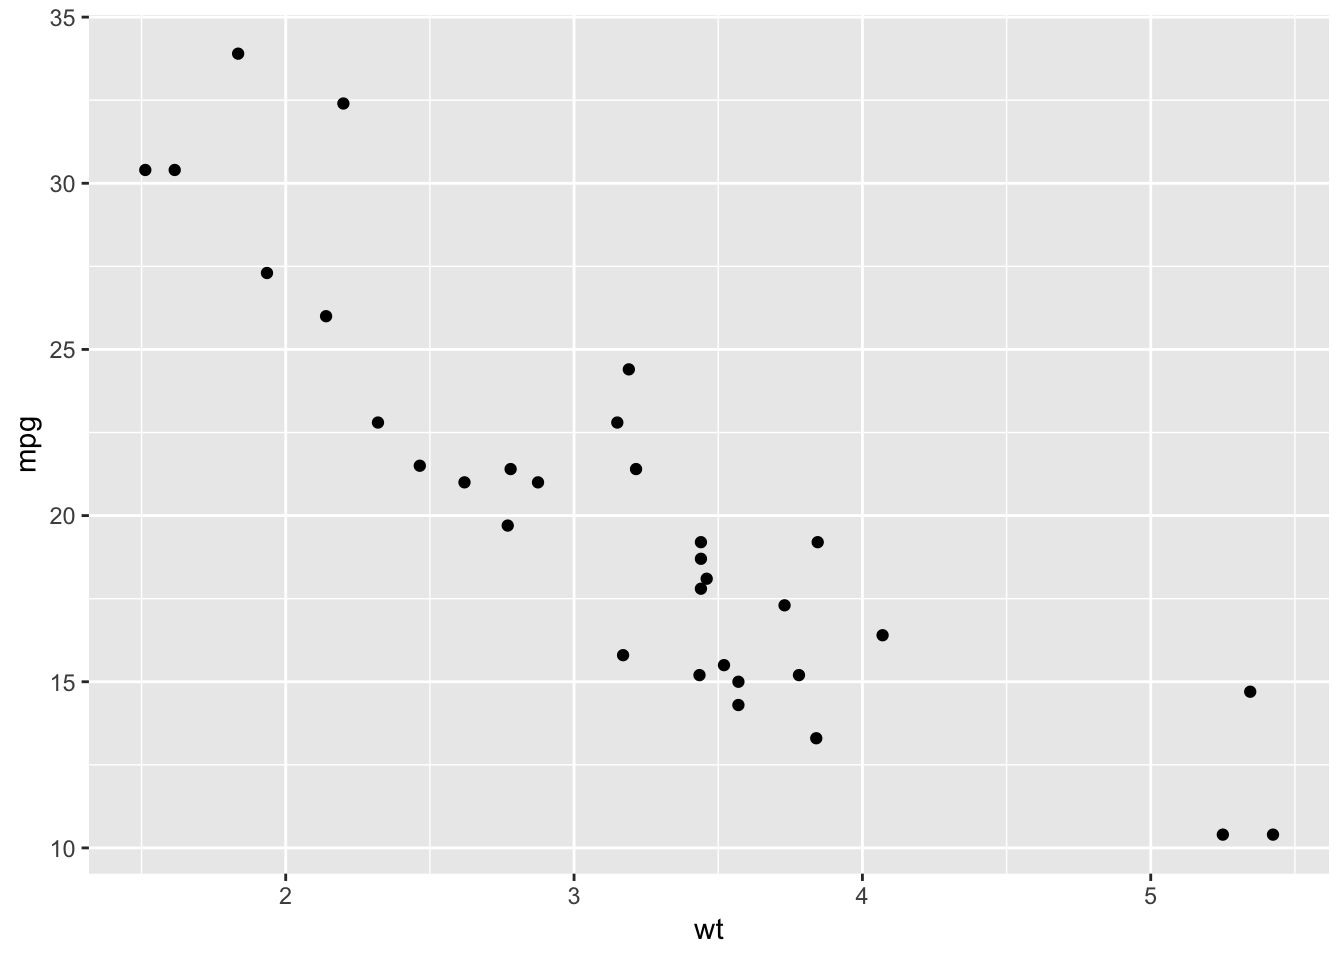
\includegraphics[height=300pt]{Day2_Dataviz_files/figure-latex/Day2-DataViz-2-1}

\begin{itemize}
\tightlist
\item
  A \texttt{data.frame} object: mtcars
\item
  Aesthetic mapping:

  \begin{itemize}
  \tightlist
  \item
    x-axis: wt
  \item
    y-axis: mpg
  \end{itemize}
\item
  Geometry:

  \begin{itemize}
  \tightlist
  \item
    geom\_point: draw points
  \end{itemize}
\end{itemize}

\begin{Shaded}
\begin{Highlighting}[]
\KeywordTok{ggplot}\NormalTok{(mtcars, }\KeywordTok{aes}\NormalTok{(}\DataTypeTok{x =}\NormalTok{ wt, }\DataTypeTok{y =}\NormalTok{ mpg)) }\OperatorTok{+}\StringTok{ }
\StringTok{  }\KeywordTok{geom_point}\NormalTok{()}\OperatorTok{+}\StringTok{ }
\StringTok{  }\KeywordTok{geom_smooth}\NormalTok{()}
\end{Highlighting}
\end{Shaded}

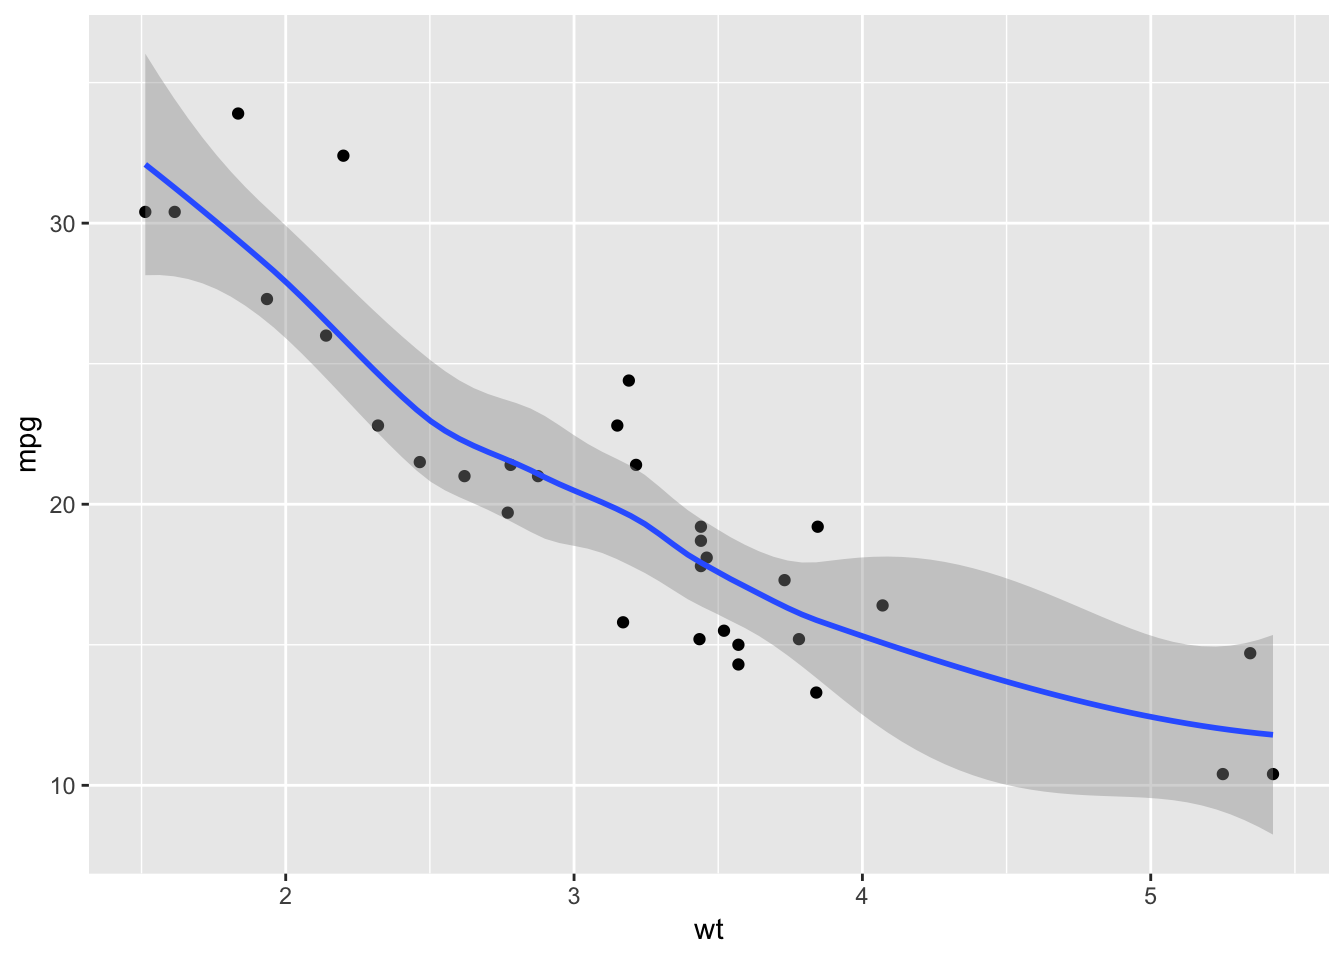
\includegraphics[height=300pt]{Day2_Dataviz_files/figure-latex/Day2-DataViz-3-1}

\begin{itemize}
\tightlist
\item
  A \texttt{data.frame} object: mtcars
\item
  Aesthetic mapping:

  \begin{itemize}
  \tightlist
  \item
    x-axis: wt
  \item
    y-axis: mpg
  \end{itemize}
\item
  Geometry:

  \begin{itemize}
  \tightlist
  \item
    geom\_point: draw points
  \item
    geom\_smooth: Add a layer which draws a best-fitting line
  \end{itemize}
\end{itemize}

Now we clean up the plot to make it presentable.

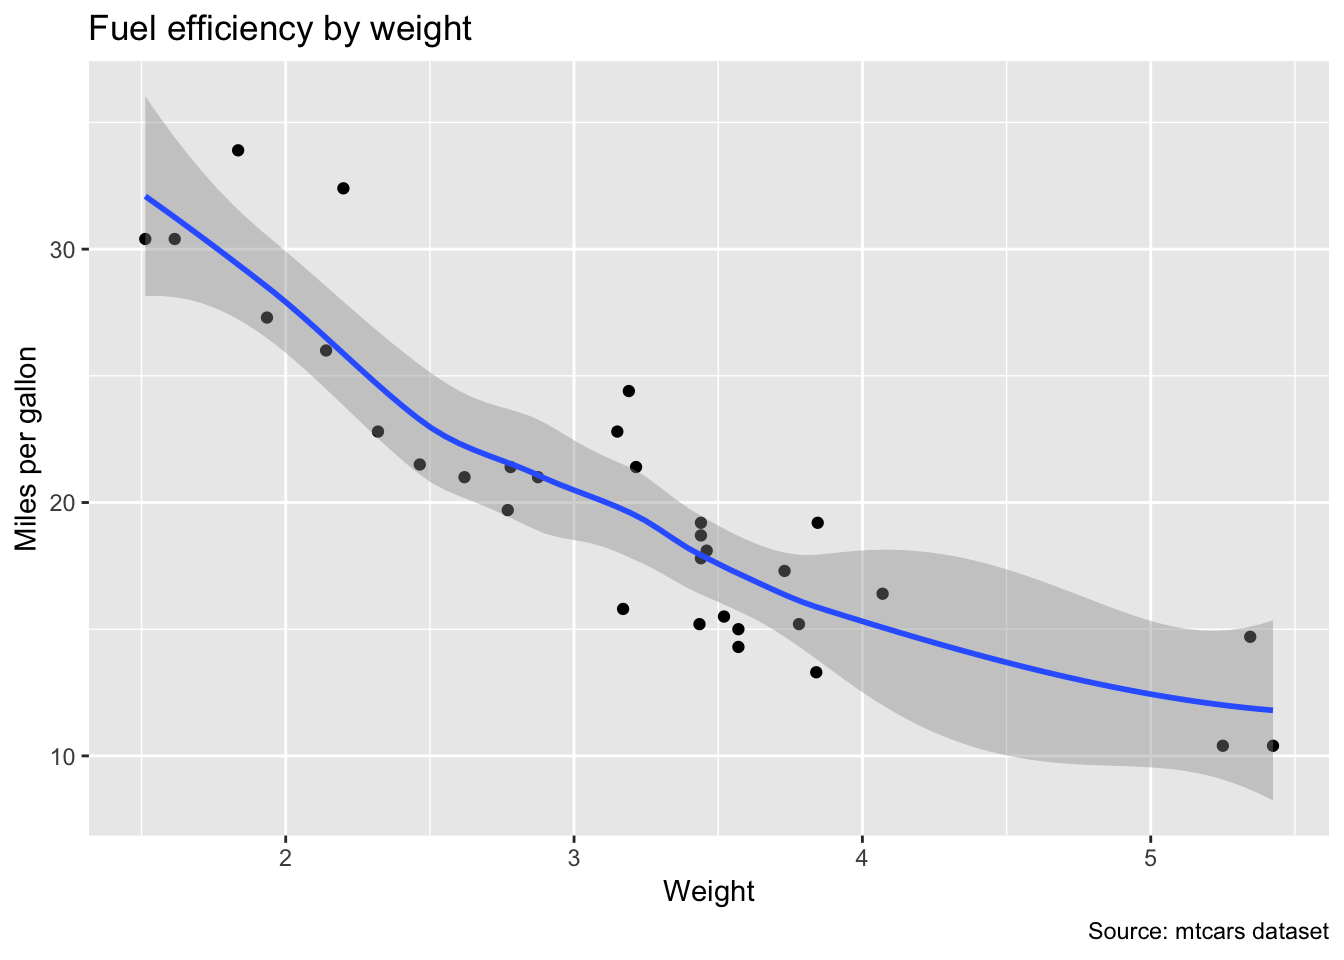
\includegraphics[height=300pt]{Day2_Dataviz_files/figure-latex/Day2-DataViz-4-1}

\hypertarget{single-continuous-variable}{%
\section{Single continuous variable}\label{single-continuous-variable}}

\hypertarget{histogram}{%
\subsection{Histogram}\label{histogram}}

\begin{Shaded}
\begin{Highlighting}[]
\NormalTok{dos <-}\StringTok{ }\KeywordTok{import}\NormalTok{(}\StringTok{'data/Department of State.csv'}\NormalTok{)}
\NormalTok{dos }\OperatorTok\StringTok{ }
\StringTok{  }\KeywordTok{ggplot}\NormalTok{(}\KeywordTok{aes}\NormalTok{(}\DataTypeTok{x =}\NormalTok{ Award_Transaction_Value)) }\OperatorTok{+}\StringTok{ }\KeywordTok{geom_histogram}\NormalTok{()}
\end{Highlighting}
\end{Shaded}

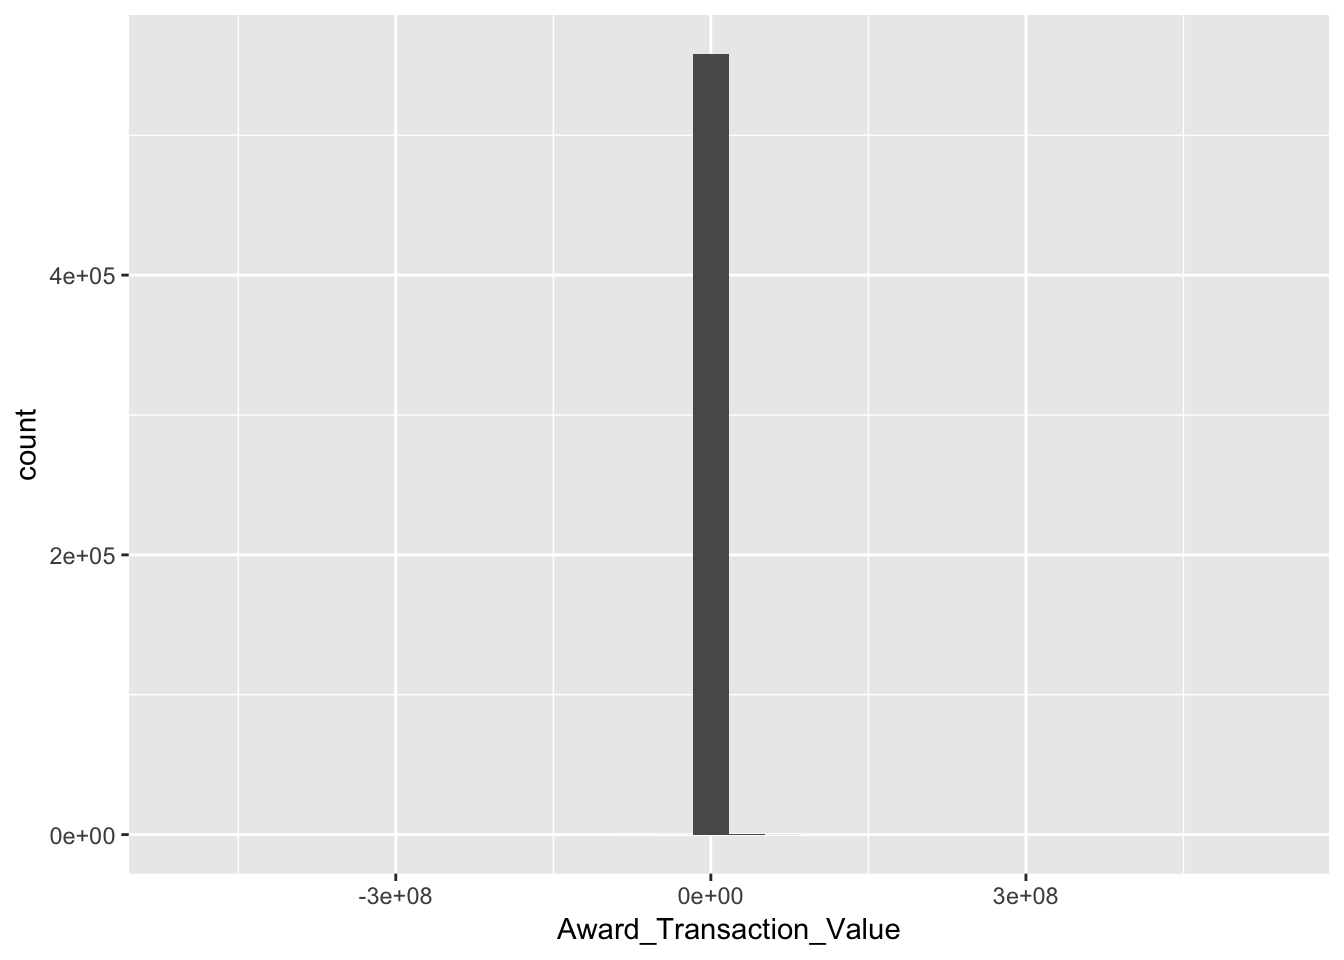
\includegraphics[height=300pt]{Day2_Dataviz_files/figure-latex/Day2-DataViz-5-1}

Change the axis to the log scale for better visual

\begin{Shaded}
\begin{Highlighting}[]
\NormalTok{dos }\OperatorTok\StringTok{ }
\StringTok{  }\KeywordTok{ggplot}\NormalTok{(}\KeywordTok{aes}\NormalTok{(}\DataTypeTok{x =}\NormalTok{ Award_Transaction_Value)) }\OperatorTok{+}\StringTok{ }\KeywordTok{geom_histogram}\NormalTok{()}\OperatorTok{+}
\StringTok{  }\KeywordTok{scale_x_log10}\NormalTok{() }\CommentTok{# x-axis on log scale}
\end{Highlighting}
\end{Shaded}

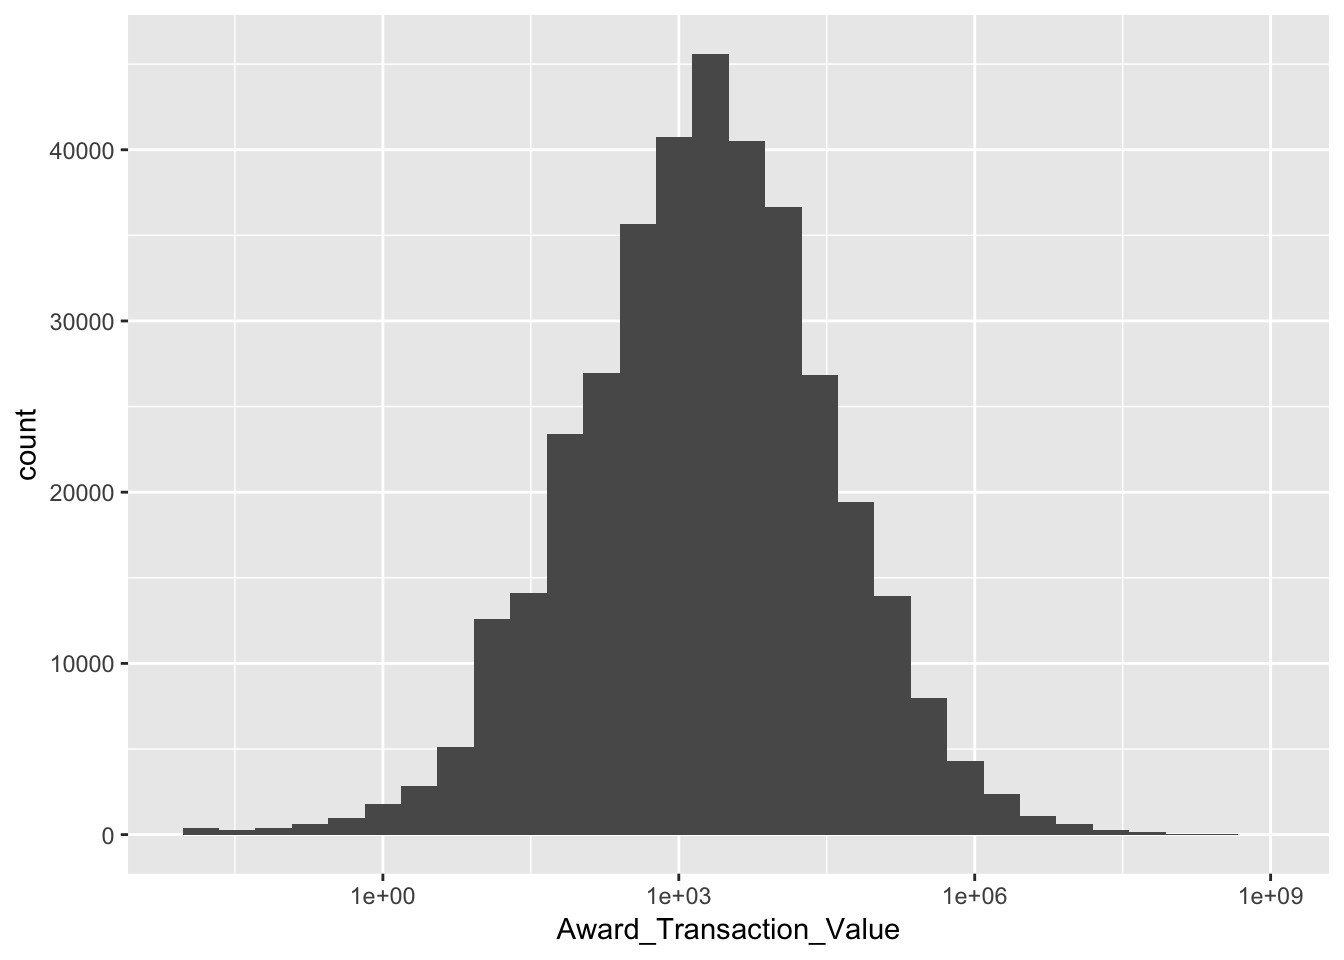
\includegraphics[height=300pt]{Day2_Dataviz_files/figure-latex/Day2-DataViz-6-1}

\hypertarget{density-plot}{%
\subsection{Density plot}\label{density-plot}}

\begin{Shaded}
\begin{Highlighting}[]
\NormalTok{dos }\OperatorTok\StringTok{ }
\StringTok{  }\KeywordTok{ggplot}\NormalTok{(}\KeywordTok{aes}\NormalTok{(}\DataTypeTok{x =}\NormalTok{ Award_Transaction_Value)) }\OperatorTok{+}\StringTok{ }\KeywordTok{geom_density}\NormalTok{()}\OperatorTok{+}
\StringTok{  }\KeywordTok{scale_x_log10}\NormalTok{()}
\end{Highlighting}
\end{Shaded}

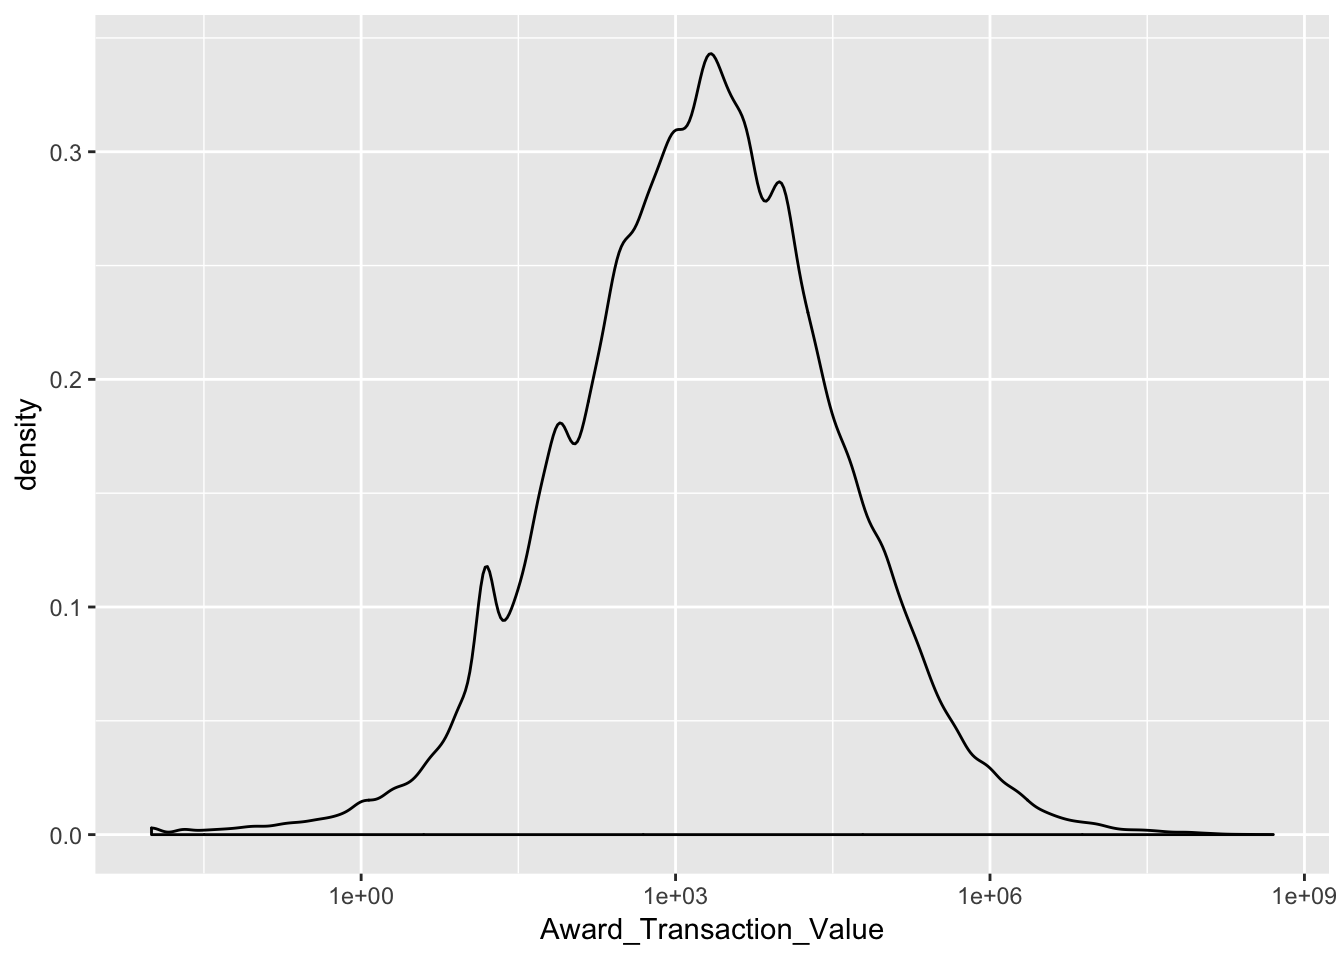
\includegraphics[height=300pt]{Day2_Dataviz_files/figure-latex/Day2-DataViz-7-1}

\hypertarget{bar-plots}{%
\section{Bar plots}\label{bar-plots}}

\begin{Shaded}
\begin{Highlighting}[]
\KeywordTok{library}\NormalTok{(lubridate)}
\NormalTok{dos }\OperatorTok\StringTok{ }
\StringTok{  }\KeywordTok{group_by}\NormalTok{(}\DataTypeTok{year =} \KeywordTok{year}\NormalTok{(}\KeywordTok{as_date}\NormalTok{(Award_Start_Date))) }\OperatorTok\StringTok{ }
\StringTok{  }\KeywordTok{summarize}\NormalTok{(}\DataTypeTok{amount =} \KeywordTok{sum}\NormalTok{(Award_Transaction_Value)) }\OperatorTok\StringTok{ }
\StringTok{  }\KeywordTok{ggplot}\NormalTok{(}\KeywordTok{aes}\NormalTok{(}\DataTypeTok{x =}\NormalTok{ year, }\DataTypeTok{y =}\NormalTok{ amount)) }\OperatorTok{+}\StringTok{ }\CommentTok{# Note change in pipe operator}
\StringTok{    }\KeywordTok{geom_bar}\NormalTok{(}\DataTypeTok{stat=}\StringTok{'identity'}\NormalTok{)}
\end{Highlighting}
\end{Shaded}

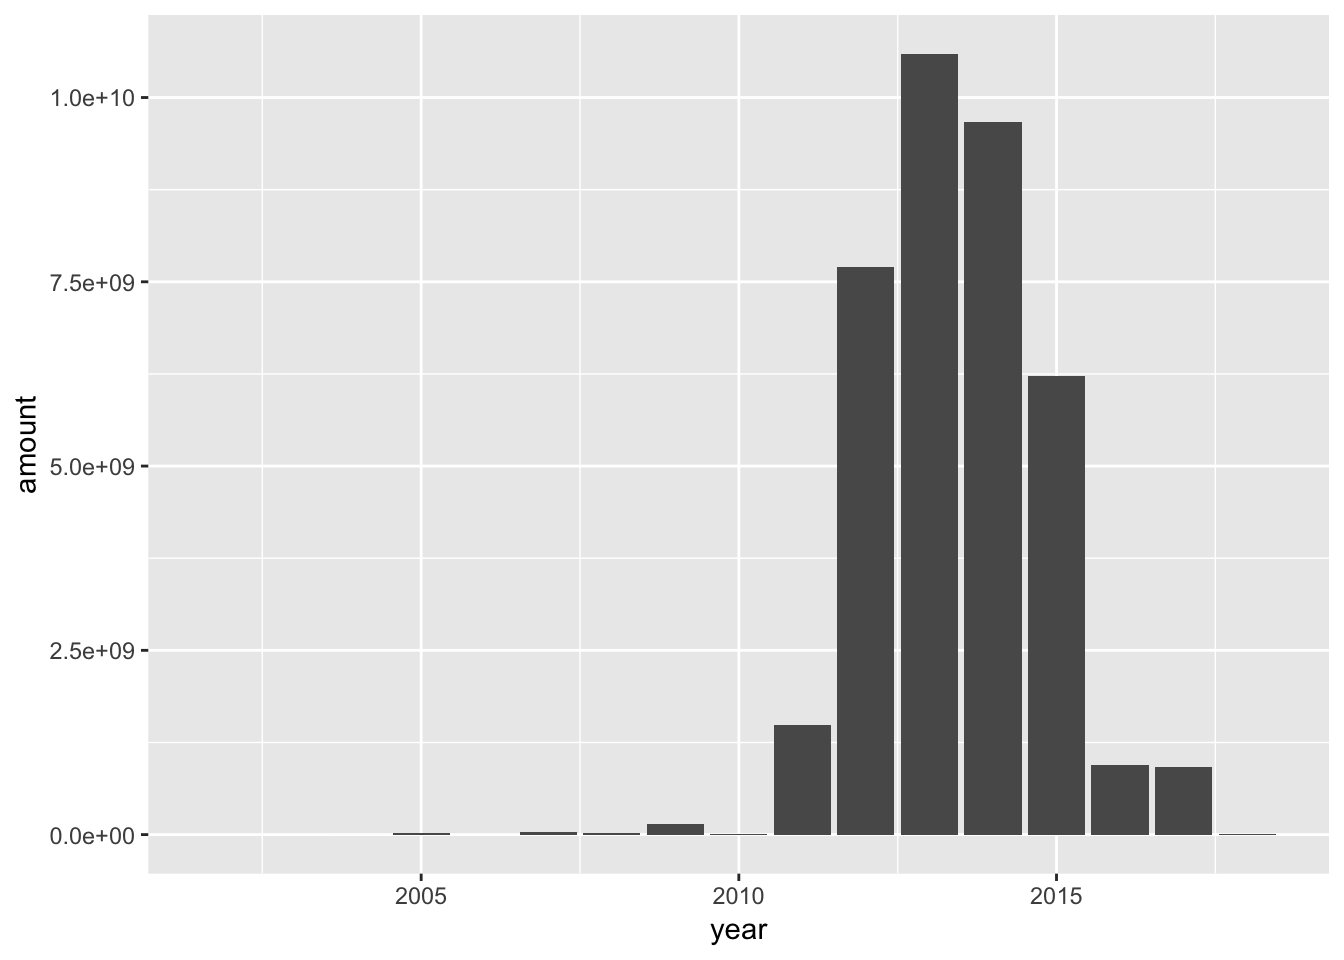
\includegraphics[height=300pt]{Day2_Dataviz_files/figure-latex/Day2-DataViz-8-1}

\hypertarget{exercise}{%
\subsection{Exercise}\label{exercise}}

Using the \texttt{mtcars} dataset in R, create:

\begin{enumerate}
\def\labelenumi{\arabic{enumi}.}
\tightlist
\item
  A histogram of the fuel efficiences (\texttt{mpg}) in the data set
\item
  A bar plot of frequencies of number of cylinders (\texttt{cyl}) in the car
\end{enumerate}

\begin{Shaded}
\begin{Highlighting}[]
\KeywordTok{ggplot}\NormalTok{(mtcars, }\KeywordTok{aes}\NormalTok{(}\DataTypeTok{x =}\NormalTok{ mpg)) }\OperatorTok{+}\StringTok{ }\KeywordTok{geom_histogram}\NormalTok{(}\DataTypeTok{binwidth=}\DecValTok{3}\NormalTok{)}
\end{Highlighting}
\end{Shaded}

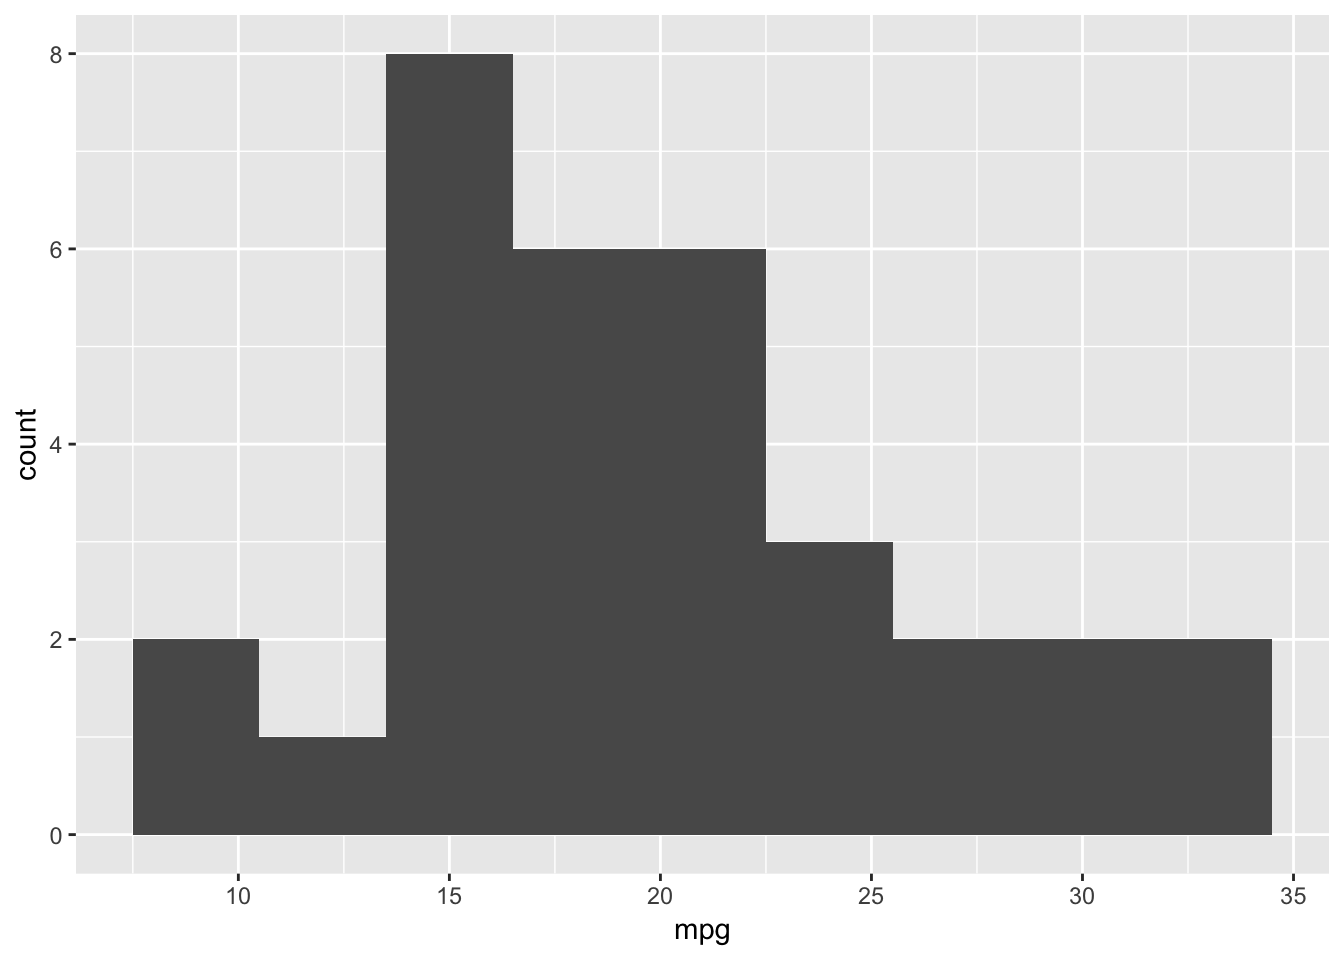
\includegraphics[height=300pt]{Day2_Dataviz_files/figure-latex/Day2-DataViz-9-1}

\begin{Shaded}
\begin{Highlighting}[]
\CommentTok{# ggplot(mtcars) + geom_histogram(aes(x = mpg), binwidth = 3)}
\end{Highlighting}
\end{Shaded}

\begin{Shaded}
\begin{Highlighting}[]
\KeywordTok{ggplot}\NormalTok{(mtcars, }\KeywordTok{aes}\NormalTok{(}\DataTypeTok{x =} \KeywordTok{factor}\NormalTok{(cyl))) }\OperatorTok{+}\StringTok{ }\KeywordTok{geom_bar}\NormalTok{()}
\end{Highlighting}
\end{Shaded}

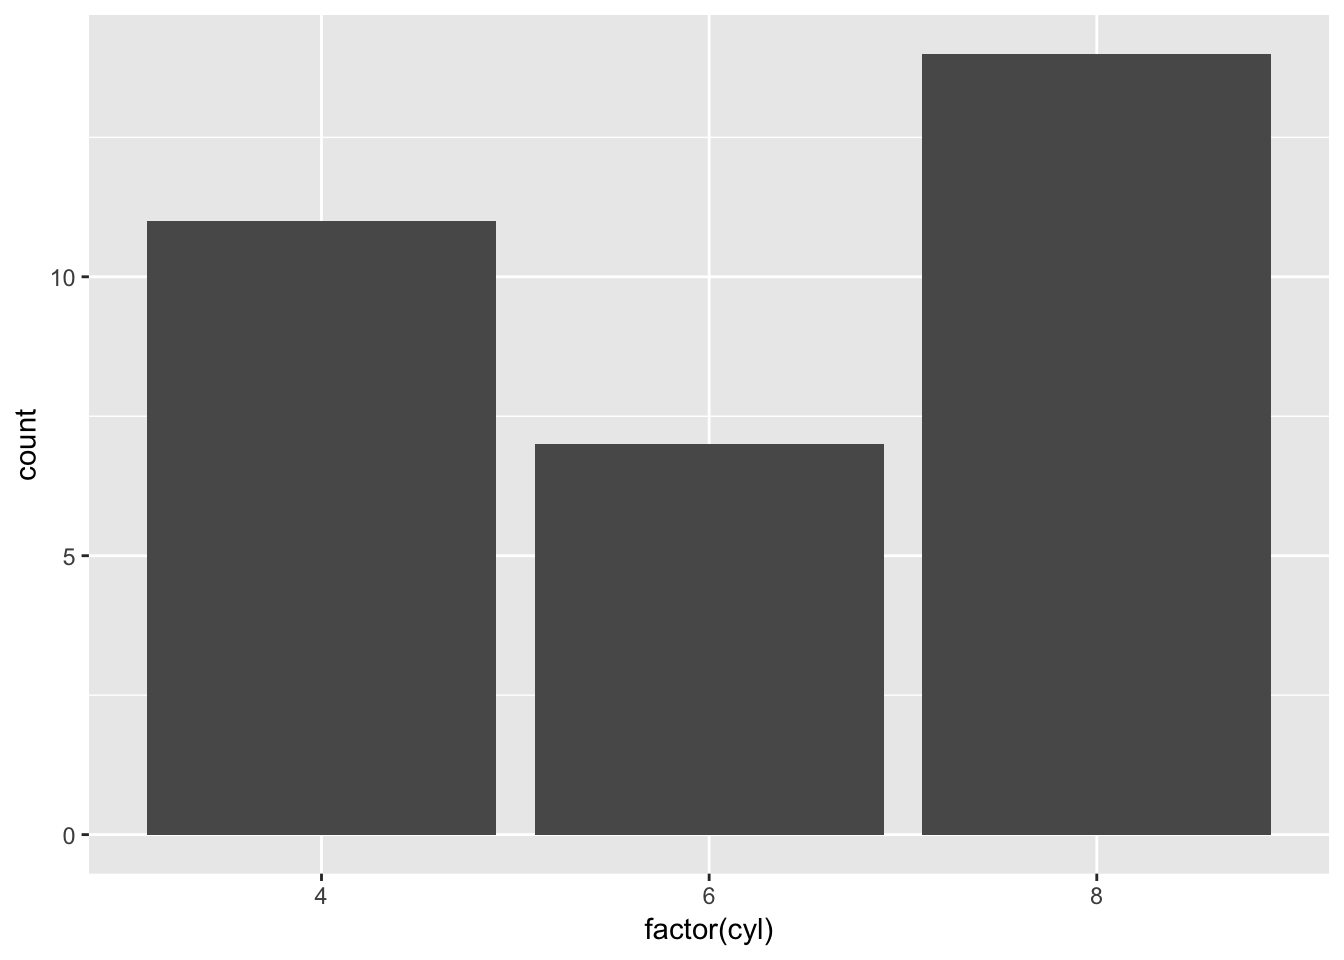
\includegraphics[height=300pt]{Day2_Dataviz_files/figure-latex/Day2-DataViz-10-1}

\hypertarget{two-continuous-variables}{%
\section{Two continuous variables}\label{two-continuous-variables}}

\hypertarget{adding-a-best-fitting-straight-line}{%
\subsection{Adding a best fitting straight line}\label{adding-a-best-fitting-straight-line}}

\begin{Shaded}
\begin{Highlighting}[]
\KeywordTok{ggplot}\NormalTok{(mtcars, }\KeywordTok{aes}\NormalTok{(}\DataTypeTok{x =}\NormalTok{ hp, }\DataTypeTok{y =}\NormalTok{ mpg))}\OperatorTok{+}
\StringTok{  }\KeywordTok{geom_point}\NormalTok{()}\OperatorTok{+}
\StringTok{  }\KeywordTok{geom_smooth}\NormalTok{(}\DataTypeTok{method =} \StringTok{'lm'}\NormalTok{)}
\end{Highlighting}
\end{Shaded}

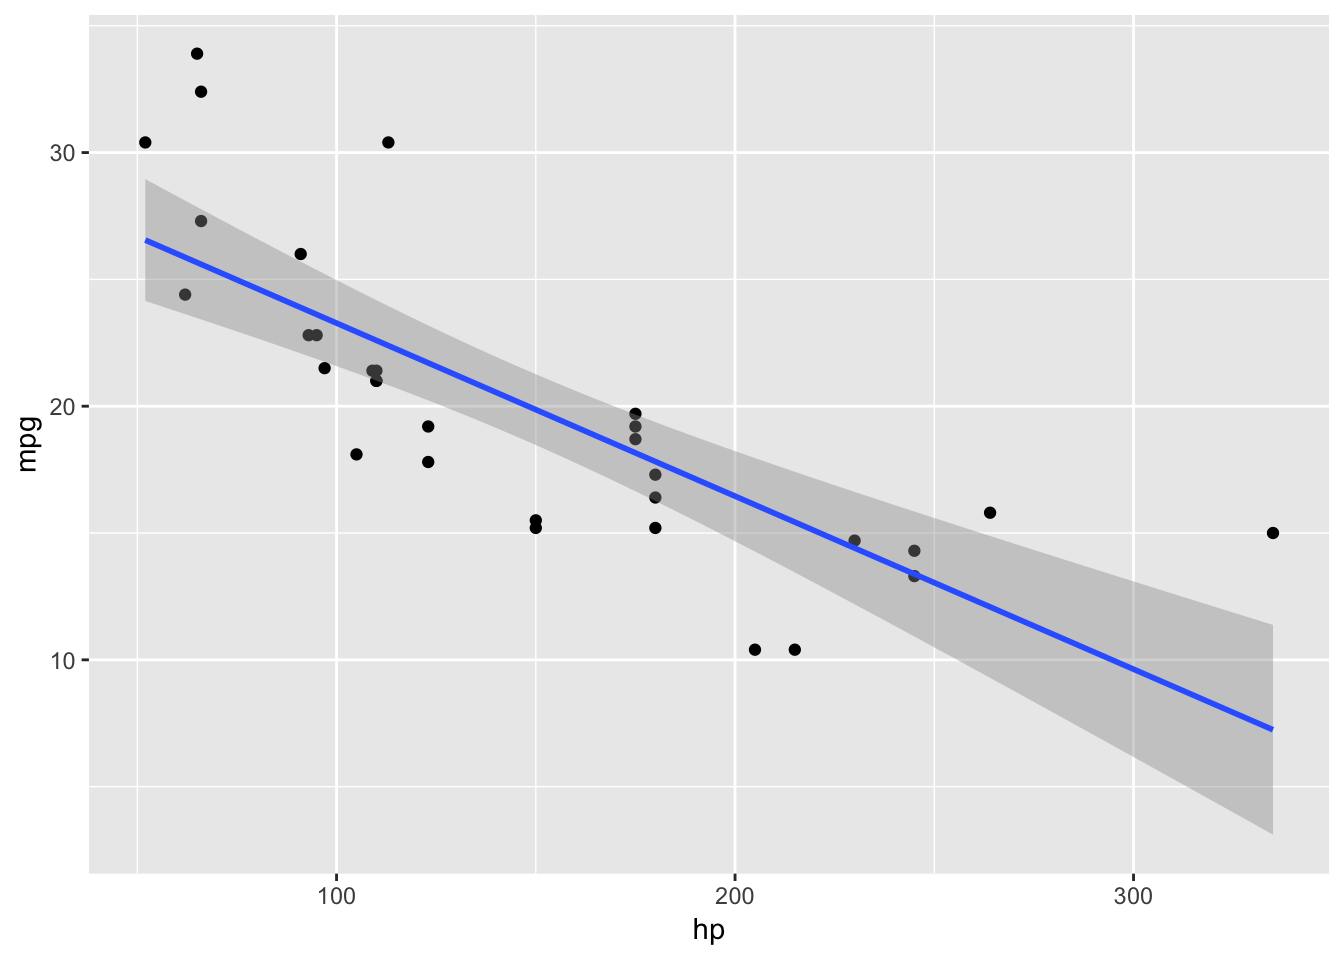
\includegraphics[height=300pt]{Day2_Dataviz_files/figure-latex/Day2-DataViz-11-1}

\hypertarget{time-series}{%
\section{Time series}\label{time-series}}

\begin{Shaded}
\begin{Highlighting}[]
\KeywordTok{library}\NormalTok{(forecast)}
\NormalTok{d <-}\StringTok{ }\KeywordTok{data.frame}\NormalTok{(}\DataTypeTok{x =} \DecValTok{1}\OperatorTok{:}\KeywordTok{length}\NormalTok{(gas), }\DataTypeTok{y =}\NormalTok{ gas) }\CommentTok{# Australian monthly gas production}
\KeywordTok{ggplot}\NormalTok{(d, }\KeywordTok{aes}\NormalTok{(x, y)) }\OperatorTok{+}\StringTok{ }\KeywordTok{geom_line}\NormalTok{()}
\end{Highlighting}
\end{Shaded}

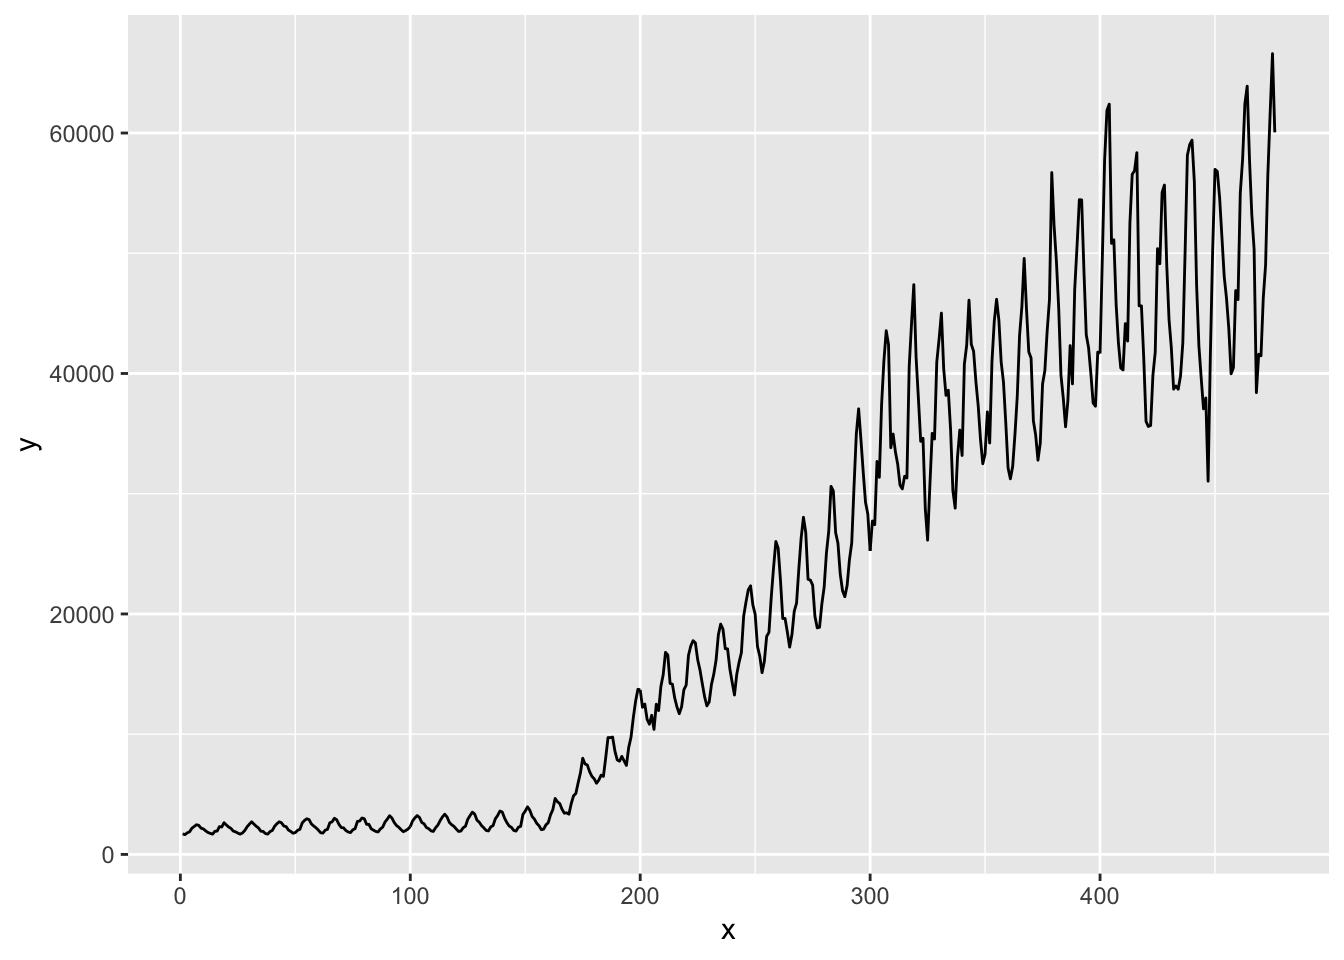
\includegraphics[height=300pt]{Day2_Dataviz_files/figure-latex/Day2-DataViz-12-1}

\hypertarget{exercise-1}{%
\subsection{Exercise}\label{exercise-1}}

\begin{enumerate}
\def\labelenumi{\arabic{enumi}.}
\tightlist
\item
  Create a scatter plot of sepal length and sepal width from the \texttt{iris} dataset, and
  add a smooth line through it
\end{enumerate}

\hypertarget{continuous-variable-with-discrete-variable}{%
\section{Continuous variable with discrete variable}\label{continuous-variable-with-discrete-variable}}

\hypertarget{boxplot}{%
\subsection{Boxplot}\label{boxplot}}

\begin{Shaded}
\begin{Highlighting}[]
\NormalTok{dos }\OperatorTok\StringTok{ }
\KeywordTok{ggplot}\NormalTok{(}\KeywordTok{aes}\NormalTok{(}\DataTypeTok{x =} \KeywordTok{factor}\NormalTok{(}\KeywordTok{year}\NormalTok{(}\KeywordTok{as_date}\NormalTok{(Award_Start_Date))),}
                \DataTypeTok{y =}\NormalTok{ Award_Transaction_Value))}\OperatorTok{+}
\StringTok{  }\KeywordTok{geom_boxplot}\NormalTok{() }\OperatorTok{+}
\StringTok{  }\KeywordTok{scale_y_log10}\NormalTok{()}\OperatorTok{+}
\StringTok{  }\KeywordTok{labs}\NormalTok{(}\DataTypeTok{x =} \StringTok{'Year'}\NormalTok{)}
\end{Highlighting}
\end{Shaded}

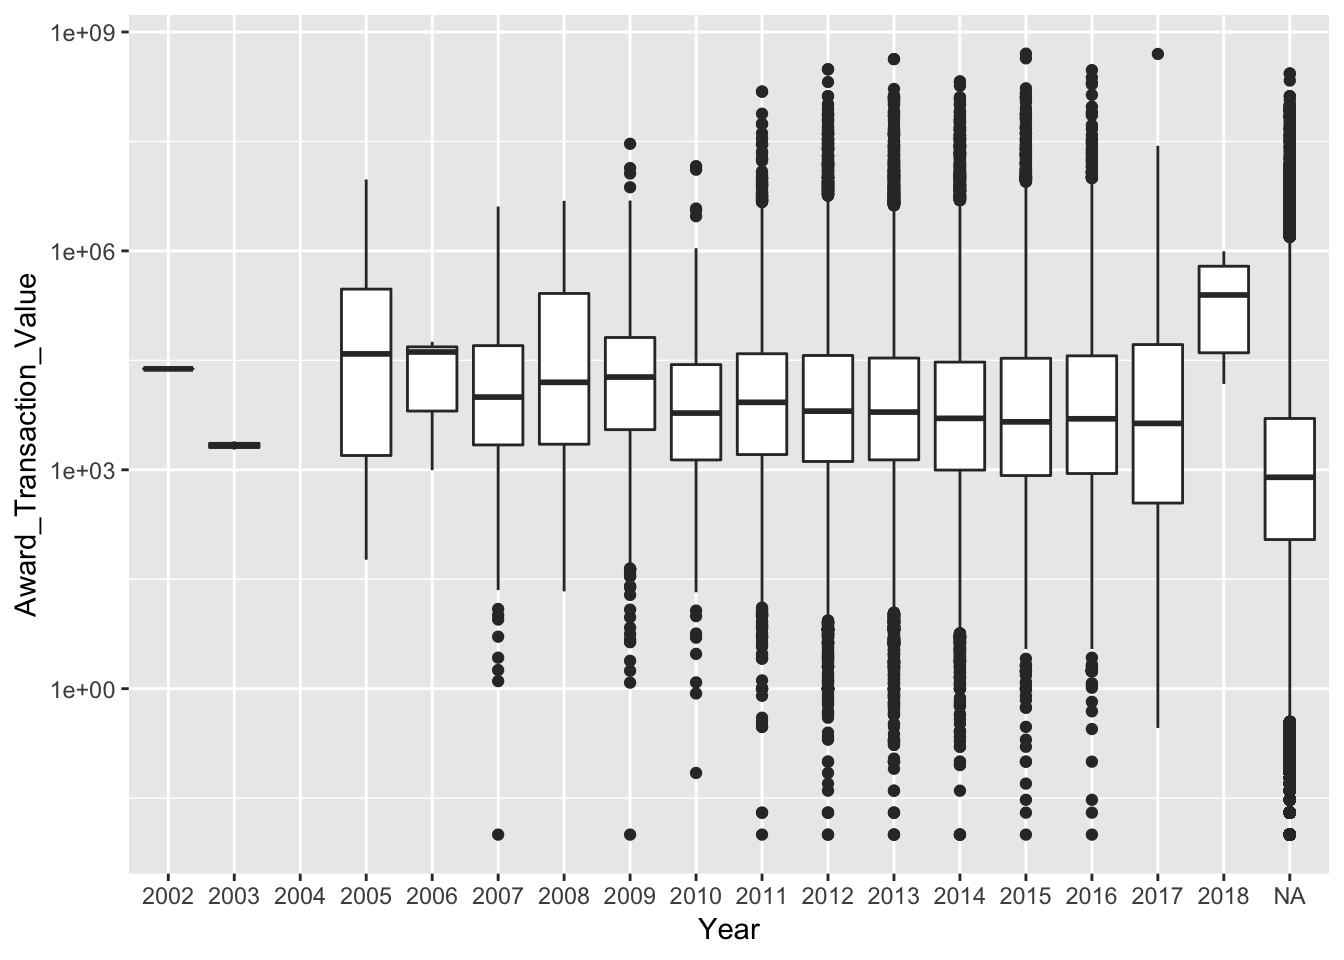
\includegraphics[height=300pt]{Day2_Dataviz_files/figure-latex/Day2-DataViz-13-1}

\hypertarget{violin-plot}{%
\subsection{Violin plot}\label{violin-plot}}

This is essetially a reflected density plot and gives a better sense of the data distribution

\begin{Shaded}
\begin{Highlighting}[]
\NormalTok{dos }\OperatorTok\StringTok{ }
\KeywordTok{ggplot}\NormalTok{(}\KeywordTok{aes}\NormalTok{(}\DataTypeTok{x =} \KeywordTok{factor}\NormalTok{(}\KeywordTok{year}\NormalTok{(}\KeywordTok{as_date}\NormalTok{(Award_Start_Date))),}
                \DataTypeTok{y =}\NormalTok{ Award_Transaction_Value))}\OperatorTok{+}
\StringTok{  }\KeywordTok{geom_violin}\NormalTok{() }\OperatorTok{+}
\StringTok{  }\KeywordTok{scale_y_log10}\NormalTok{()}\OperatorTok{+}
\StringTok{  }\KeywordTok{labs}\NormalTok{(}\DataTypeTok{x =} \StringTok{'Year'}\NormalTok{)}
\end{Highlighting}
\end{Shaded}

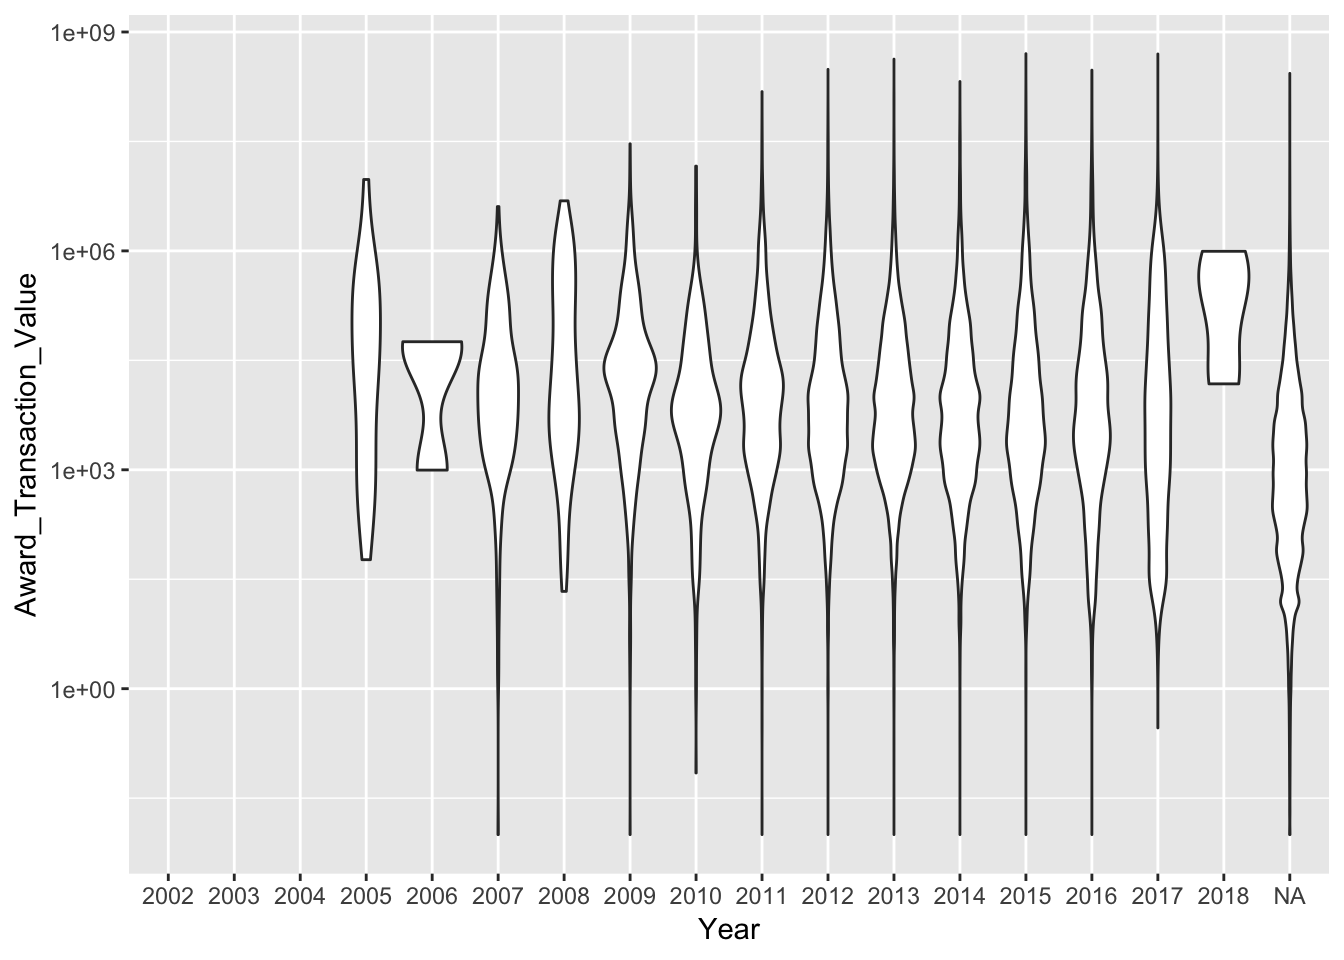
\includegraphics[height=300pt]{Day2_Dataviz_files/figure-latex/Day2-DataViz-14-1}

\hypertarget{exercise-2}{%
\subsection{Exercise}\label{exercise-2}}

\begin{enumerate}
\def\labelenumi{\arabic{enumi}.}
\tightlist
\item
  Plot a boxplot of petal length by species using the \texttt{iris} dataset
\end{enumerate}

\hypertarget{grouped-visualizations}{%
\section{Grouped visualizations}\label{grouped-visualizations}}

We're going to plot the change in aid provided to each country over time. To do
this we need summaries by time and location

\begin{Shaded}
\begin{Highlighting}[]
\NormalTok{grp_data <-}\StringTok{ }\NormalTok{dos }\OperatorTok\StringTok{ }
\StringTok{  }\KeywordTok{group_by}\NormalTok{(Recipient_Location, }\DataTypeTok{year =} \KeywordTok{year}\NormalTok{(}\KeywordTok{as_date}\NormalTok{(Award_Start_Date))) }\OperatorTok\StringTok{ }
\StringTok{  }\KeywordTok{summarize}\NormalTok{(}\DataTypeTok{amt =} \KeywordTok{sum}\NormalTok{(Award_Transaction_Value)) }\OperatorTok\StringTok{ }
\StringTok{  }\KeywordTok{filter}\NormalTok{(}\KeywordTok{str_detect}\NormalTok{(Recipient_Location, }\StringTok{'^C'}\NormalTok{))}
\KeywordTok{ggplot}\NormalTok{(grp_data, }\KeywordTok{aes}\NormalTok{(}\DataTypeTok{x =}\NormalTok{ year, }\DataTypeTok{y =}\NormalTok{ amt, }\DataTypeTok{color=}\NormalTok{Recipient_Location))}\OperatorTok{+}
\StringTok{  }\KeywordTok{geom_line}\NormalTok{()}\OperatorTok{+}
\StringTok{  }\KeywordTok{scale_y_log10}\NormalTok{()}
\end{Highlighting}
\end{Shaded}

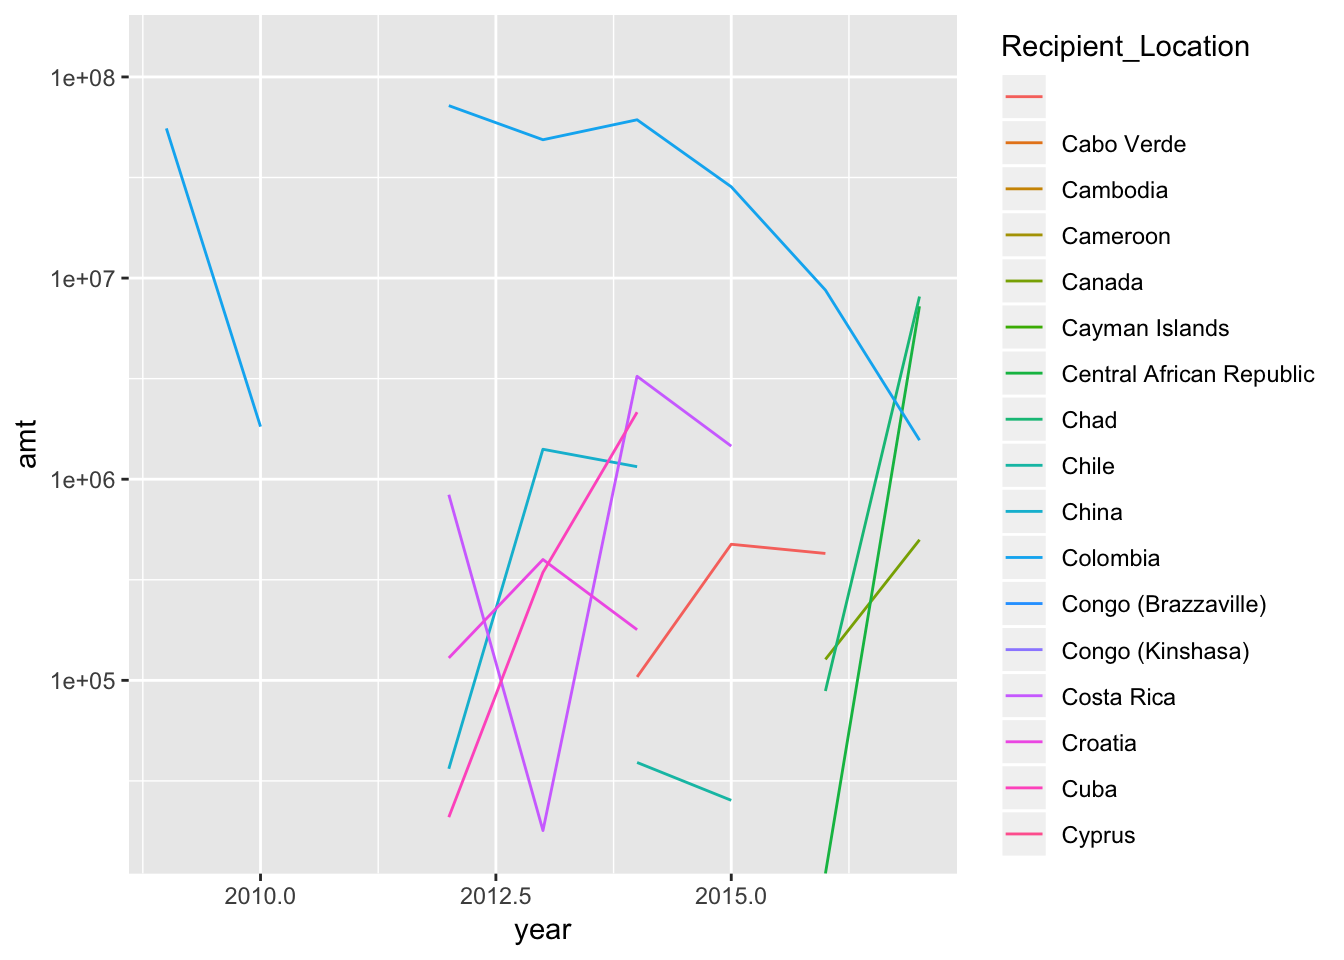
\includegraphics[height=300pt]{Day2_Dataviz_files/figure-latex/Day2-DataViz-15-1}

\begin{Shaded}
\begin{Highlighting}[]
\KeywordTok{ggplot}\NormalTok{(grp_data, }\KeywordTok{aes}\NormalTok{(}\DataTypeTok{x =}\NormalTok{ year,  }\DataTypeTok{y =}\NormalTok{ amt))}\OperatorTok{+}
\StringTok{  }\KeywordTok{geom_line}\NormalTok{()}\OperatorTok{+}
\StringTok{  }\KeywordTok{scale_y_log10}\NormalTok{()}\OperatorTok{+}
\StringTok{  }\KeywordTok{facet_wrap}\NormalTok{(}\OperatorTok{~}\NormalTok{Recipient_Location)}
\end{Highlighting}
\end{Shaded}

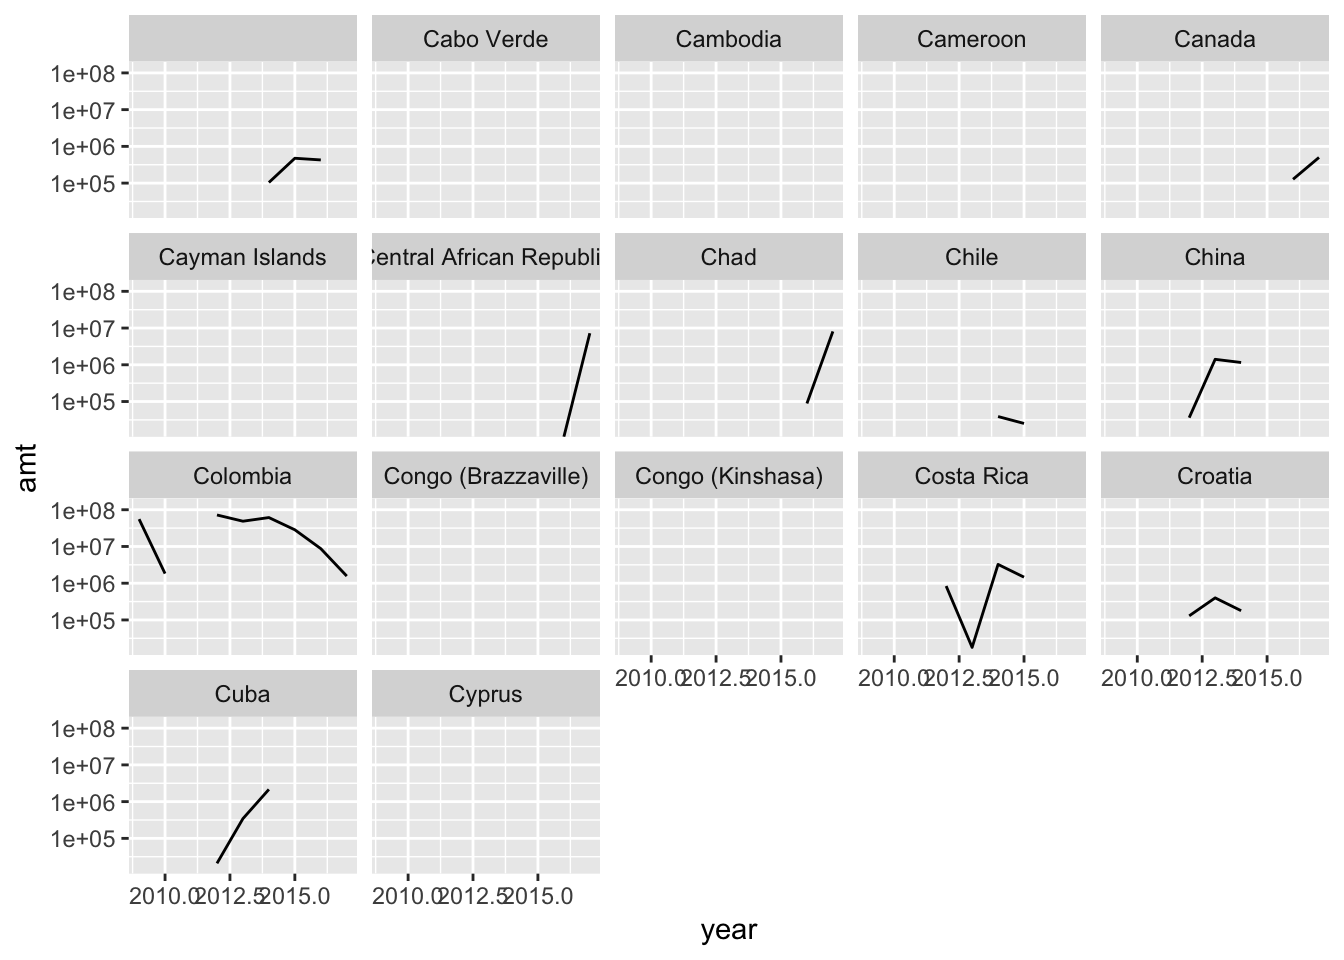
\includegraphics[height=300pt]{Day2_Dataviz_files/figure-latex/Day2-DataViz-16-1}

\begin{Shaded}
\begin{Highlighting}[]
\CommentTok{## dos %>% filter(str_detect(Recipient_Location, '^C')) %>%}
\CommentTok{## ggplot(aes(x = year(as_date(Award_Start_Date)),}
\CommentTok{##            y = Award_Transaction_Value,}
\CommentTok{##            color = Recipient_Location,}
\CommentTok{##            shape = Award_Transaction_Type))+}
\CommentTok{##   geom_point()+}
\CommentTok{##   labs(x = 'Year', color='Location')+}
\CommentTok{##   scale_y_log10()}
\CommentTok{## }
\end{Highlighting}
\end{Shaded}

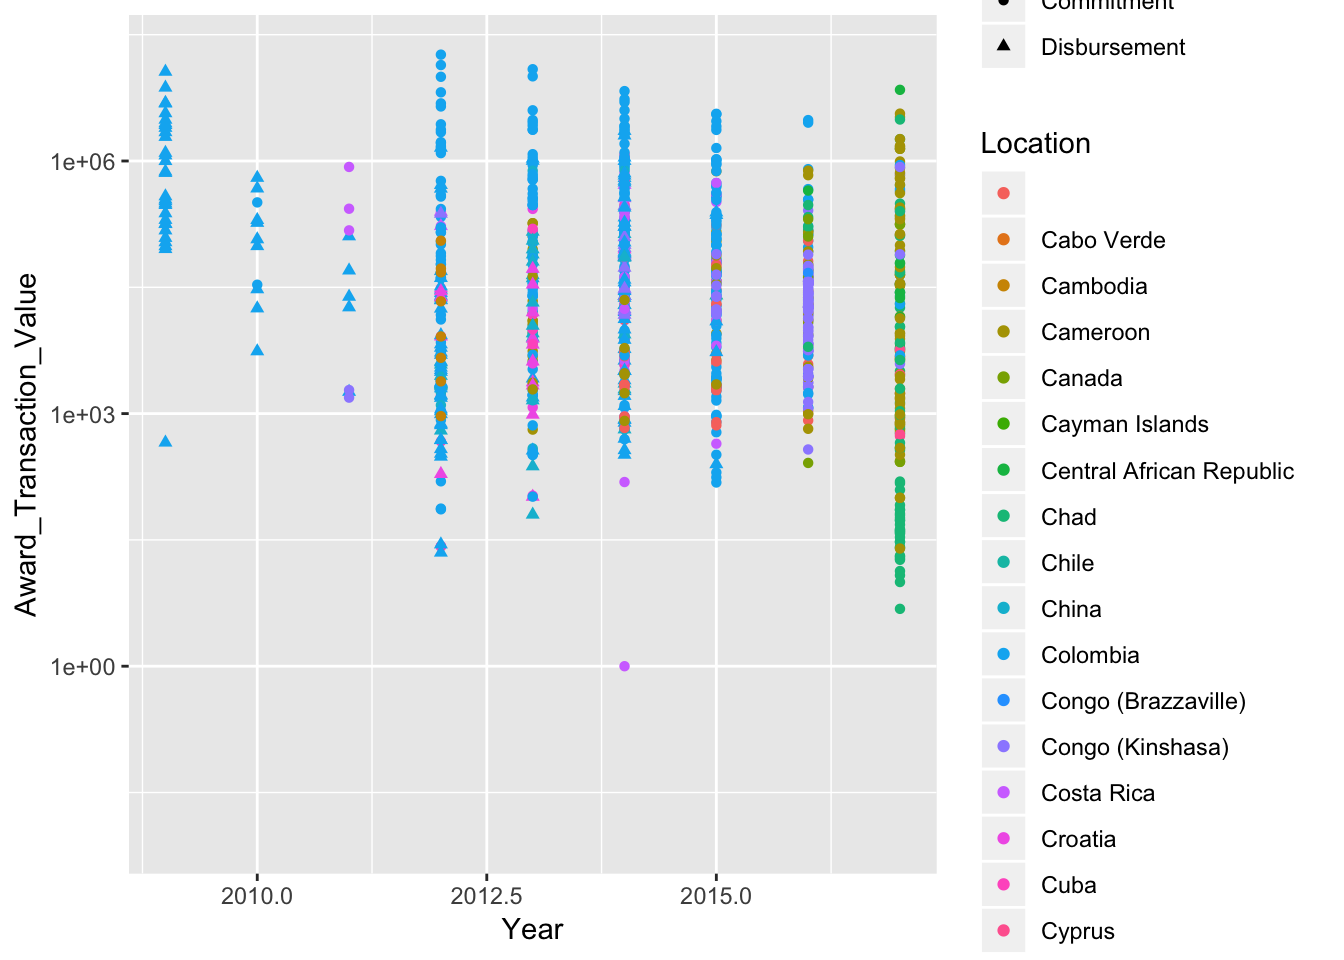
\includegraphics[height=300pt]{Day2_Dataviz_files/figure-latex/Day2-DataViz-18-1}

\begin{Shaded}
\begin{Highlighting}[]
\CommentTok{## dos %>% filter(str_detect(Recipient_Location, '^C')) %>%}
\CommentTok{## ggplot(aes(x = year(as_date(Award_Start_Date)),}
\CommentTok{##            y = Award_Transaction_Value,}
\CommentTok{##            color = Recipient_Location,}
\CommentTok{##            shape = Award_Transaction_Type))+}
\CommentTok{##   geom_jitter()+}
\CommentTok{##   labs(x = 'Year', color='Location')+}
\CommentTok{##   scale_y_log10()}
\CommentTok{## }
\end{Highlighting}
\end{Shaded}

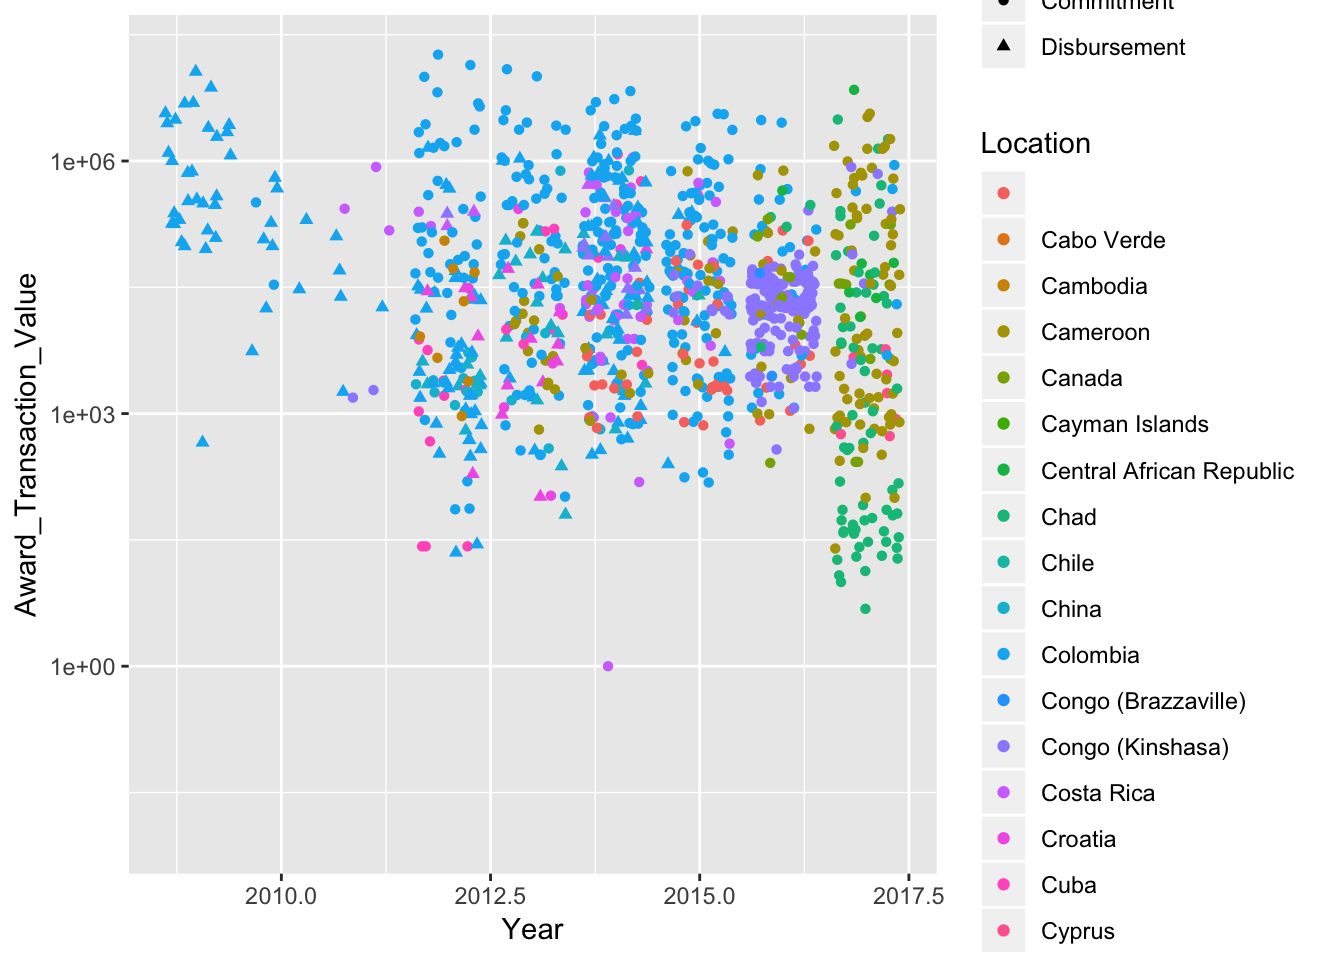
\includegraphics[height=300pt]{Day2_Dataviz_files/figure-latex/Day2-DataViz-20-1}

\begin{Shaded}
\begin{Highlighting}[]
\NormalTok{schools <-}\StringTok{ }\NormalTok{rio}\OperatorTok{::}\KeywordTok{import}\NormalTok{(}\StringTok{'data/schools.rds'}\NormalTok{)}
\NormalTok{schools }\OperatorTok\StringTok{ }\KeywordTok{filter}\NormalTok{(tophead}\OperatorTok{==}\StringTok{'Elementary schools'}\NormalTok{, }
\NormalTok{                   head2}\OperatorTok{==}\StringTok{"Average hours in school day"}\NormalTok{) }\OperatorTok\StringTok{ }
\StringTok{  }\KeywordTok{filter}\NormalTok{(}\OperatorTok{!}\KeywordTok{is.na}\NormalTok{(State), State }\OperatorTok{!=}\StringTok{ 'United States'}\NormalTok{) }\OperatorTok\StringTok{ }
\StringTok{  }\KeywordTok{ggplot}\NormalTok{(}\KeywordTok{aes}\NormalTok{(}\DataTypeTok{x =}\NormalTok{ State, }\DataTypeTok{y =}\NormalTok{ stats, }\DataTypeTok{ymin =}\NormalTok{ stats }\OperatorTok{-}\StringTok{ }\DecValTok{2}\OperatorTok{*}\NormalTok{se, }
             \DataTypeTok{ymax =}\NormalTok{ stats }\OperatorTok{+}\StringTok{ }\DecValTok{2}\OperatorTok{*}\NormalTok{se)) }\OperatorTok{+}
\StringTok{  }\KeywordTok{geom_pointrange}\NormalTok{()}\OperatorTok{+}
\StringTok{  }\KeywordTok{labs}\NormalTok{(}\DataTypeTok{y =} \StringTok{'Avg hours in school day'}\NormalTok{)}\OperatorTok{+}
\StringTok{  }\KeywordTok{theme_bw}\NormalTok{()}\OperatorTok{+}
\StringTok{  }\KeywordTok{theme}\NormalTok{(}\DataTypeTok{axis.text.x =} \KeywordTok{element_text}\NormalTok{(}\DataTypeTok{angle=}\DecValTok{45}\NormalTok{, }\DataTypeTok{hjust =} \DecValTok{1}\NormalTok{))}
\end{Highlighting}
\end{Shaded}

\hypertarget{maps}{%
\section{Maps}\label{maps}}

\begin{center}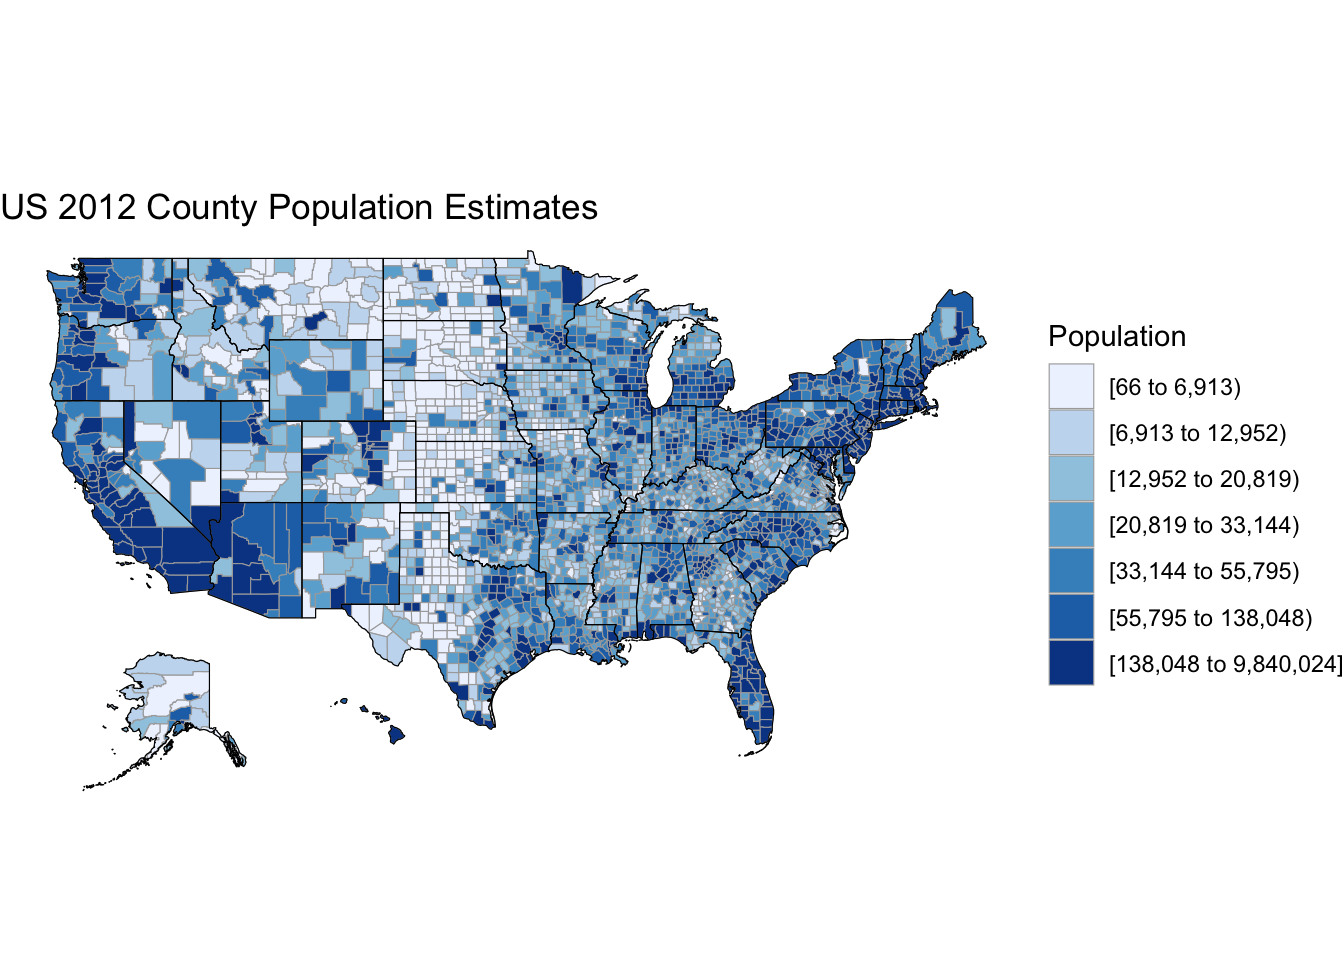
\includegraphics[height=600pt]{Day2_Dataviz_files/figure-latex/Day2-DataViz-22-1} \end{center}

We can also ingest SHP files to draw maps. We don't show the final version since
it took too long to render.

\begin{Shaded}
\begin{Highlighting}[]
\KeywordTok{library}\NormalTok{(sf)}
\NormalTok{hrr_info <-}\StringTok{ }\KeywordTok{st_read}\NormalTok{(}\StringTok{'~/Downloads/hrr_bdry-1/HRR_Bdry.SHP'}\NormalTok{)}
\KeywordTok{head}\NormalTok{(hrr_info)}
\KeywordTok{ggplot}\NormalTok{(hrr_info)}\OperatorTok{+}\KeywordTok{geom_sf}\NormalTok{()}
\KeywordTok{ggsave}\NormalTok{(}\StringTok{'map.png'}\NormalTok{)}
\end{Highlighting}
\end{Shaded}

\hypertarget{stitching-graphs-together.}{%
\section{Stitching graphs together.}\label{stitching-graphs-together.}}

\begin{Shaded}
\begin{Highlighting}[]
\CommentTok{# install.packages('cowplot')}
\KeywordTok{library}\NormalTok{(cowplot)}
\NormalTok{p1 <-}\StringTok{ }\KeywordTok{ggplot}\NormalTok{(iris, }\KeywordTok{aes}\NormalTok{(Sepal.Length, Sepal.Width, }\DataTypeTok{color =}\NormalTok{ Species)) }\OperatorTok{+}
\StringTok{ }\KeywordTok{geom_point}\NormalTok{() }\OperatorTok{+}\StringTok{ }\KeywordTok{facet_grid}\NormalTok{(. }\OperatorTok{~}\StringTok{ }\NormalTok{Species) }\OperatorTok{+}\StringTok{ }\KeywordTok{stat_smooth}\NormalTok{(}\DataTypeTok{method =} \StringTok{"lm"}\NormalTok{) }\OperatorTok{+}
\StringTok{ }\KeywordTok{background_grid}\NormalTok{(}\DataTypeTok{major =} \StringTok{'y'}\NormalTok{, }\DataTypeTok{minor =} \StringTok{"none"}\NormalTok{) }\OperatorTok{+}
\StringTok{ }\KeywordTok{panel_border}\NormalTok{() }\OperatorTok{+}\StringTok{ }\KeywordTok{theme}\NormalTok{(}\DataTypeTok{legend.position =} \StringTok{"none"}\NormalTok{)}

\CommentTok{# plot B}
\NormalTok{p2 <-}\StringTok{ }\KeywordTok{ggplot}\NormalTok{(iris, }\KeywordTok{aes}\NormalTok{(Sepal.Length, }\DataTypeTok{fill =}\NormalTok{ Species)) }\OperatorTok{+}
\StringTok{ }\KeywordTok{geom_density}\NormalTok{(}\DataTypeTok{alpha =} \FloatTok{.7}\NormalTok{) }\OperatorTok{+}\StringTok{ }\KeywordTok{theme}\NormalTok{(}\DataTypeTok{legend.justification =} \StringTok{"top"}\NormalTok{)}
\NormalTok{p2a <-}\StringTok{ }\NormalTok{p2 }\OperatorTok{+}\StringTok{ }\KeywordTok{theme}\NormalTok{(}\DataTypeTok{legend.position =} \StringTok{"none"}\NormalTok{)}

\CommentTok{# plot C}
\NormalTok{p3 <-}\StringTok{ }\KeywordTok{ggplot}\NormalTok{(iris, }\KeywordTok{aes}\NormalTok{(Sepal.Width, }\DataTypeTok{fill =}\NormalTok{ Species)) }\OperatorTok{+}
\StringTok{ }\KeywordTok{geom_density}\NormalTok{(}\DataTypeTok{alpha =} \FloatTok{.7}\NormalTok{) }\OperatorTok{+}\StringTok{ }\KeywordTok{theme}\NormalTok{(}\DataTypeTok{legend.position =} \StringTok{"none"}\NormalTok{)}

\CommentTok{# legend}
\NormalTok{legend <-}\StringTok{ }\KeywordTok{get_legend}\NormalTok{(p2)}

\CommentTok{# align all plots vertically}
\NormalTok{plots <-}\StringTok{ }\KeywordTok{align_plots}\NormalTok{(p1, p2a, p3, }\DataTypeTok{align =} \StringTok{'v'}\NormalTok{, }\DataTypeTok{axis =} \StringTok{'l'}\NormalTok{)}

\CommentTok{# put together bottom row and then everything}
\NormalTok{bottom_row <-}\StringTok{ }\KeywordTok{plot_grid}\NormalTok{(plots[[}\DecValTok{2}\NormalTok{]], plots[[}\DecValTok{3}\NormalTok{]], legend, }\DataTypeTok{labels =} \KeywordTok{c}\NormalTok{(}\StringTok{"B"}\NormalTok{, }\StringTok{"C"}\NormalTok{), }\DataTypeTok{rel_widths =} \KeywordTok{c}\NormalTok{(}\DecValTok{1}\NormalTok{, }\DecValTok{1}\NormalTok{, }\FloatTok{.3}\NormalTok{), }\DataTypeTok{nrow =} \DecValTok{1}\NormalTok{)}
\KeywordTok{plot_grid}\NormalTok{(plots[[}\DecValTok{1}\NormalTok{]], bottom_row, }\DataTypeTok{labels =} \KeywordTok{c}\NormalTok{(}\StringTok{"A"}\NormalTok{), }\DataTypeTok{ncol =} \DecValTok{1}\NormalTok{)}
\end{Highlighting}
\end{Shaded}

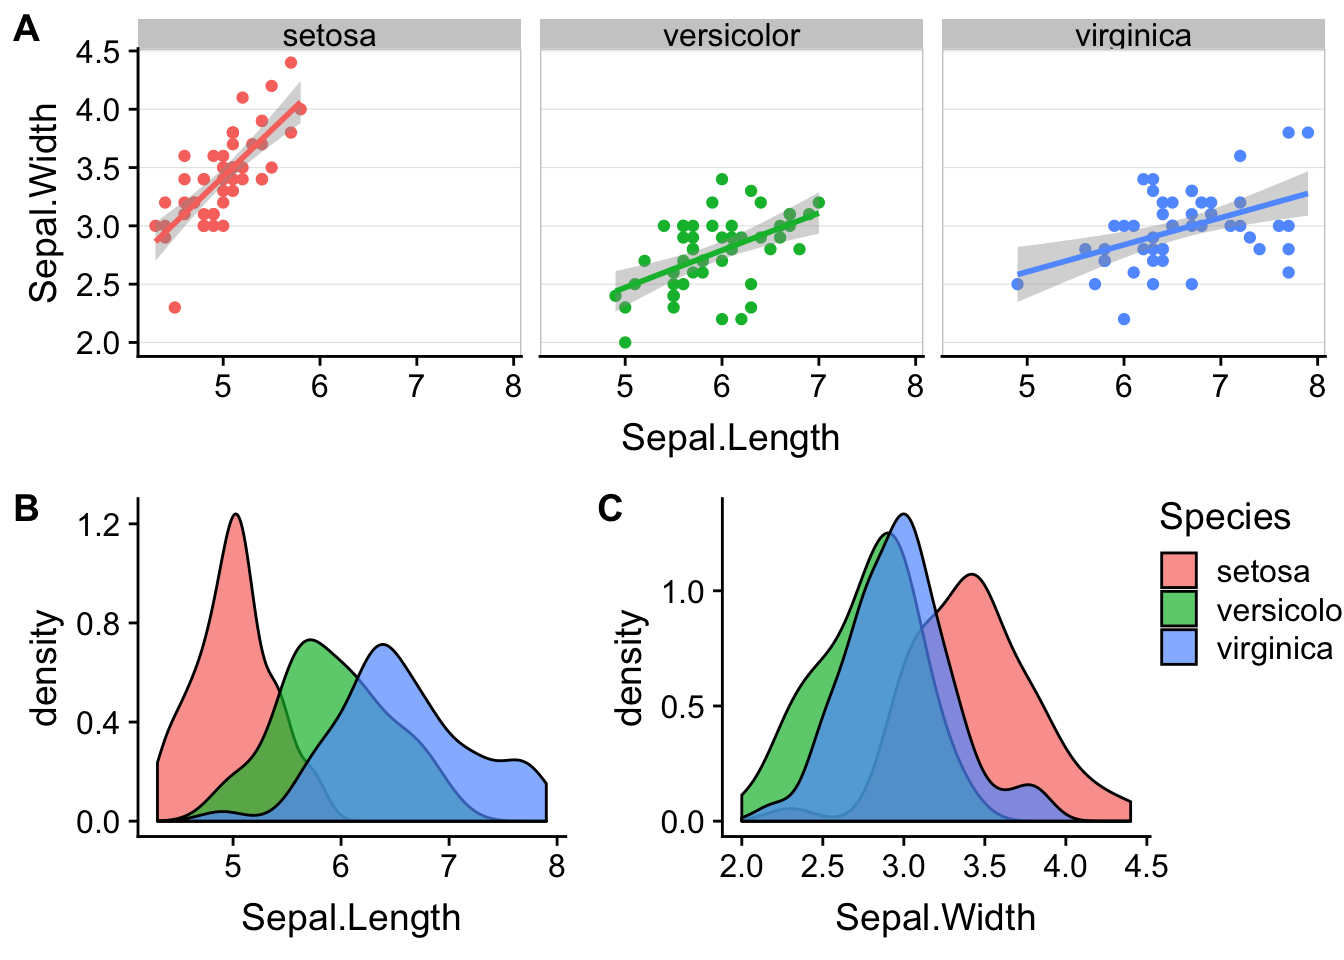
\includegraphics[height=300pt]{Day2_Dataviz_files/figure-latex/Day2-DataViz-24-1}

\begin{Shaded}
\begin{Highlighting}[]
\CommentTok{## library(ggplot2)}
\CommentTok{## library(plotly)}
\CommentTok{## p=ggplot(iris, aes(x=Sepal.Length,}
\CommentTok{##                    y=Sepal.Width,}
\CommentTok{##                    color=Species,}
\CommentTok{##                    shape=Species)) +}
\CommentTok{##     geom_point(size=6, alpha=0.6)}
\CommentTok{## mytext=paste("Sepal Length = ", iris$Sepal.Length,}
\CommentTok{##              "\textbackslash{}n" , "Sepal Width = ", iris$Sepal.Width,}
\CommentTok{##              "\textbackslash{}n", "Row Number: ",rownames(iris),  sep="")}
\CommentTok{## pp=plotly::plotly_build(p)}
\CommentTok{## style( pp, text=mytext,}
\CommentTok{##        hoverinfo = "text",}
\CommentTok{##        traces = c(1, 2, 3) )}
\end{Highlighting}
\end{Shaded}

\hypertarget{interactive}{%
\section{Interactive graphics}\label{interactive}}

We won't put these in the notes, since they don't work well in printed form

\hypertarget{functions}{%
\chapter{Functions}\label{functions}}

\begin{Shaded}
\begin{Highlighting}[]
\NormalTok{myDumbFunction <-}\StringTok{ }\ControlFlowTok{function}\NormalTok{() }\DecValTok{42}
\KeywordTok{myDumbFunction}\NormalTok{()}
\end{Highlighting}
\end{Shaded}

\begin{verbatim}
[1] 42
\end{verbatim}

\begin{Shaded}
\begin{Highlighting}[]
\NormalTok{doubleIt <-}\StringTok{ }\ControlFlowTok{function}\NormalTok{(x) \{}
\NormalTok{  myResult <-}\StringTok{ }\NormalTok{x }\OperatorTok{*}\StringTok{ }\DecValTok{2}
\NormalTok{  myResult }\CommentTok{# or, explicitly, return(myResult)}
\NormalTok{\}}
\KeywordTok{doubleIt}\NormalTok{(}\DecValTok{5}\NormalTok{)}
\end{Highlighting}
\end{Shaded}

\begin{verbatim}
[1] 10
\end{verbatim}

\begin{Shaded}
\begin{Highlighting}[]
\KeywordTok{exists}\NormalTok{(}\StringTok{"myResult"}\NormalTok{)}
\end{Highlighting}
\end{Shaded}

\begin{verbatim}
[1] FALSE
\end{verbatim}

\begin{Shaded}
\begin{Highlighting}[]
\NormalTok{myResult <-}\StringTok{ }\DecValTok{1000}
\NormalTok{doubleItOutput <-}\StringTok{ }\KeywordTok{doubleIt}\NormalTok{(}\DecValTok{2}\NormalTok{)}
\NormalTok{myResult}
\end{Highlighting}
\end{Shaded}

\begin{verbatim}
[1] 1000
\end{verbatim}

\begin{Shaded}
\begin{Highlighting}[]
\NormalTok{my_sum <-}\StringTok{ }\ControlFlowTok{function}\NormalTok{(x)\{}
\NormalTok{  s <-}\StringTok{ }\KeywordTok{sum}\NormalTok{(x)}
\NormalTok{  n <-}\StringTok{ }\KeywordTok{length}\NormalTok{(x)}
\NormalTok{  result <-}\StringTok{ }\NormalTok{s }\OperatorTok{/}\StringTok{ }\NormalTok{n}
  \KeywordTok{return}\NormalTok{(result)}
\NormalTok{\}}
\end{Highlighting}
\end{Shaded}

\begin{Shaded}
\begin{Highlighting}[]
\KeywordTok{my_sum}\NormalTok{(}\DecValTok{1}\OperatorTok{:}\DecValTok{10}\NormalTok{)}
\end{Highlighting}
\end{Shaded}

\begin{verbatim}
[1] 5.5
\end{verbatim}

\begin{Shaded}
\begin{Highlighting}[]
\NormalTok{answer <-}\StringTok{ }\KeywordTok{my_sum}\NormalTok{(}\DecValTok{1}\OperatorTok{:}\DecValTok{10}\NormalTok{)}
\NormalTok{answer}
\end{Highlighting}
\end{Shaded}

\begin{verbatim}
[1] 5.5
\end{verbatim}

\begin{Shaded}
\begin{Highlighting}[]
\NormalTok{my_sum <-}\StringTok{ }\ControlFlowTok{function}\NormalTok{(x)\{}
\NormalTok{  s <-}\StringTok{ }\KeywordTok{sum}\NormalTok{(x)}
\NormalTok{  n <-}\StringTok{ }\KeywordTok{length}\NormalTok{(x)}
\NormalTok{  results<-}\StringTok{ }\KeywordTok{list}\NormalTok{(}\DataTypeTok{sum =}\NormalTok{ s, }\DataTypeTok{length =}\NormalTok{ n, }\DataTypeTok{answer =}\NormalTok{ s }\OperatorTok{/}\StringTok{ }\NormalTok{n)}
  \KeywordTok{return}\NormalTok{(results)}
\NormalTok{\}}
\end{Highlighting}
\end{Shaded}

\begin{Shaded}
\begin{Highlighting}[]
\KeywordTok{my_sum}\NormalTok{(}\DecValTok{1}\OperatorTok{:}\DecValTok{10}\NormalTok{) }
\end{Highlighting}
\end{Shaded}

\begin{verbatim}
$sum
[1] 55

$length
[1] 10

$answer
[1] 5.5
\end{verbatim}

\begin{Shaded}
\begin{Highlighting}[]
\NormalTok{my_sum <-}\StringTok{ }\ControlFlowTok{function}\NormalTok{(x)\{}
\NormalTok{  s <-}\StringTok{ }\KeywordTok{sum}\NormalTok{(x)}
\NormalTok{  n <-}\StringTok{ }\KeywordTok{length}\NormalTok{(x)}
\NormalTok{  results<-}\StringTok{ }\KeywordTok{list}\NormalTok{(}\DataTypeTok{sum =}\NormalTok{ s, }\DataTypeTok{length =}\NormalTok{ n, }\DataTypeTok{answer =}\NormalTok{ s }\OperatorTok{/}\StringTok{ }\NormalTok{n)}
  \KeywordTok{return}\NormalTok{(results)}
\NormalTok{\}}
\end{Highlighting}
\end{Shaded}

\begin{Shaded}
\begin{Highlighting}[]
\NormalTok{answer <-}\StringTok{ }\KeywordTok{my_sum}\NormalTok{(}\DecValTok{1}\OperatorTok{:}\DecValTok{10}\NormalTok{)}
\NormalTok{answer}\OperatorTok{$}\NormalTok{answer}
\end{Highlighting}
\end{Shaded}

\begin{verbatim}
[1] 5.5
\end{verbatim}

\begin{Shaded}
\begin{Highlighting}[]
\NormalTok{answer[[}\StringTok{'answer'}\NormalTok{]]}
\end{Highlighting}
\end{Shaded}

\begin{verbatim}
[1] 5.5
\end{verbatim}

\begin{Shaded}
\begin{Highlighting}[]
\KeywordTok{names}\NormalTok{(answer)}
\end{Highlighting}
\end{Shaded}

\begin{verbatim}
[1] "sum"    "length" "answer"
\end{verbatim}

\begin{Shaded}
\begin{Highlighting}[]
\NormalTok{x <-}\StringTok{ }\DecValTok{1}\OperatorTok{:}\DecValTok{10}
\NormalTok{x[}\DecValTok{3}\NormalTok{] <-}\StringTok{ }\OtherTok{NA}
\KeywordTok{my_sum}\NormalTok{(x)}
\end{Highlighting}
\end{Shaded}

\begin{verbatim}
$sum
[1] NA

$length
[1] 10

$answer
[1] NA
\end{verbatim}

\begin{Shaded}
\begin{Highlighting}[]
\NormalTok{my_sum <-}\StringTok{ }\ControlFlowTok{function}\NormalTok{(x)\{}
\NormalTok{  s <-}\StringTok{ }\KeywordTok{sum}\NormalTok{(x, }\DataTypeTok{na.rm=}\NormalTok{T)}
\NormalTok{  n <-}\StringTok{ }\KeywordTok{length}\NormalTok{(}\OperatorTok{!}\KeywordTok{is.na}\NormalTok{(x))}
\NormalTok{  results <-}\StringTok{ }\KeywordTok{list}\NormalTok{(}\StringTok{"sum"}\NormalTok{ =}\StringTok{ }\NormalTok{s, }\StringTok{"length"}\NormalTok{ =}\StringTok{ }\NormalTok{n, }\StringTok{"answer"}\NormalTok{ =}\StringTok{ }\NormalTok{s}\OperatorTok{/}\NormalTok{n)}
\NormalTok{\}}
\KeywordTok{my_sum}\NormalTok{(x)}
\end{Highlighting}
\end{Shaded}

\begin{Shaded}
\begin{Highlighting}[]
\NormalTok{my_sum <-}\StringTok{ }\ControlFlowTok{function}\NormalTok{(x)\{}
\NormalTok{  s <-}\StringTok{ }\KeywordTok{sum}\NormalTok{(x, }\DataTypeTok{na.rm =}\NormalTok{ T)}
\NormalTok{  n <-}\StringTok{ }\KeywordTok{length}\NormalTok{(}\OperatorTok{!}\KeywordTok{is.na}\NormalTok{(x))}
\NormalTok{  results <-}\StringTok{ }\KeywordTok{list}\NormalTok{(}\StringTok{"sum"}\NormalTok{ =}\StringTok{ }\NormalTok{s, }\StringTok{"length"}\NormalTok{ =}\StringTok{ }\NormalTok{n, }\StringTok{"answer"}\NormalTok{ =}\StringTok{ }\NormalTok{s}\OperatorTok{/}\NormalTok{n)}
  \KeywordTok{return}\NormalTok{(results) }\CommentTok{#<<}
\NormalTok{\}}
\KeywordTok{my_sum}\NormalTok{(x)}
\end{Highlighting}
\end{Shaded}

\begin{verbatim}
$sum
[1] 52

$length
[1] 10

$answer
[1] 5.2
\end{verbatim}

\begin{Shaded}
\begin{Highlighting}[]
\NormalTok{my_sum <-}\StringTok{ }\ControlFlowTok{function}\NormalTok{(x)\{}
\NormalTok{  s <-}\StringTok{ }\KeywordTok{sum}\NormalTok{(x, }\DataTypeTok{na.rm =}\NormalTok{ T)}
\NormalTok{  n <-}\StringTok{ }\KeywordTok{length}\NormalTok{(}\OperatorTok{!}\KeywordTok{is.na}\NormalTok{(x)) }
\NormalTok{  results <-}\StringTok{ }\KeywordTok{list}\NormalTok{(}\StringTok{"sum"}\NormalTok{ =}\StringTok{ }\NormalTok{s, }\StringTok{"length"}\NormalTok{ =}\StringTok{ }\NormalTok{n, }\StringTok{"answer"}\NormalTok{ =}\StringTok{ }\NormalTok{s}\OperatorTok{/}\NormalTok{n)}
  \KeywordTok{return}\NormalTok{(results) }
\NormalTok{\}}
\end{Highlighting}
\end{Shaded}

\begin{Shaded}
\begin{Highlighting}[]
\NormalTok{my_sum <-}\StringTok{ }\ControlFlowTok{function}\NormalTok{(x)\{}
\NormalTok{  s <-}\StringTok{ }\KeywordTok{sum}\NormalTok{(x, }\DataTypeTok{na.rm =}\NormalTok{ T)}
\NormalTok{\{\{  n <-}\StringTok{ }\KeywordTok{sum}\NormalTok{(}\OperatorTok{!}\KeywordTok{is.na}\NormalTok{(x)) \}\}}
\NormalTok{  results <-}\StringTok{ }\KeywordTok{list}\NormalTok{(}\StringTok{"sum"}\NormalTok{ =}\StringTok{ }\NormalTok{s, }\StringTok{"length"}\NormalTok{ =}\StringTok{ }\NormalTok{n, }\StringTok{"answer"}\NormalTok{ =}\StringTok{ }\NormalTok{s}\OperatorTok{/}\NormalTok{n)}
  \KeywordTok{return}\NormalTok{(results) }
\NormalTok{\}}
\KeywordTok{my_sum}\NormalTok{(x)}
\end{Highlighting}
\end{Shaded}

\begin{verbatim}
$sum
[1] 52

$length
[1] 9

$answer
[1] 5.777778
\end{verbatim}

\begin{Shaded}
\begin{Highlighting}[]
\NormalTok{my_sum <-}\StringTok{ }\ControlFlowTok{function}\NormalTok{(x)\{}
\NormalTok{  s <-}\StringTok{ }\KeywordTok{sum}\NormalTok{(x, }\DataTypeTok{na.rm =}\NormalTok{ T)}
\NormalTok{  n <-}\StringTok{ }\KeywordTok{sum}\NormalTok{(}\OperatorTok{!}\KeywordTok{is.na}\NormalTok{(x)) }
\NormalTok{  results <-}\StringTok{ }\KeywordTok{list}\NormalTok{(}\StringTok{"sum"}\NormalTok{ =}\StringTok{ }\NormalTok{s, }\StringTok{"length"}\NormalTok{ =}\StringTok{ }\NormalTok{n, }\StringTok{"answer"}\NormalTok{ =}\StringTok{ }\NormalTok{s}\OperatorTok{/}\NormalTok{n)}
  \KeywordTok{return}\NormalTok{(results) }
\NormalTok{\}}
\end{Highlighting}
\end{Shaded}

\begin{Shaded}
\begin{Highlighting}[]
\NormalTok{my_sum <-}\StringTok{ }\ControlFlowTok{function}\NormalTok{(x, }\DataTypeTok{remove_missing =} \OtherTok{TRUE}\NormalTok{)\{ }\CommentTok{#<<}
\NormalTok{  s <-}\StringTok{ }\KeywordTok{sum}\NormalTok{(x, }\DataTypeTok{na.rm =}\NormalTok{ T)}
\NormalTok{  n <-}\StringTok{ }\KeywordTok{sum}\NormalTok{(}\OperatorTok{!}\KeywordTok{is.na}\NormalTok{(x)) }
\NormalTok{  results <-}\StringTok{ }\KeywordTok{list}\NormalTok{(}\StringTok{"sum"}\NormalTok{ =}\StringTok{ }\NormalTok{s, }\StringTok{"length"}\NormalTok{ =}\StringTok{ }\NormalTok{n, }\StringTok{"answer"}\NormalTok{ =}\StringTok{ }\NormalTok{s}\OperatorTok{/}\NormalTok{n)}
  \KeywordTok{return}\NormalTok{(results) }
\NormalTok{\}}
\end{Highlighting}
\end{Shaded}

\begin{Shaded}
\begin{Highlighting}[]
\NormalTok{my_sum <-}\StringTok{ }\ControlFlowTok{function}\NormalTok{(x, }\DataTypeTok{remove_missing =} \OtherTok{TRUE}\NormalTok{)\{ }
\NormalTok{  \{\{}\ControlFlowTok{if}\NormalTok{(remove_missing)\{}
\NormalTok{    x <-}\StringTok{ }\NormalTok{x[}\OperatorTok{!}\KeywordTok{is.na}\NormalTok{(x)]}
\NormalTok{  \}}
\NormalTok{  s <-}\StringTok{ }\KeywordTok{sum}\NormalTok{(x)}
\NormalTok{  n <-}\StringTok{ }\KeywordTok{length}\NormalTok{(x)\}\}}
\NormalTok{  results <-}\StringTok{ }\KeywordTok{list}\NormalTok{(}\StringTok{"sum"}\NormalTok{ =}\StringTok{ }\NormalTok{s, }\StringTok{"length"}\NormalTok{ =}\StringTok{ }\NormalTok{n, }\StringTok{"answer"}\NormalTok{ =}\StringTok{ }\NormalTok{s}\OperatorTok{/}\NormalTok{n)}
  \KeywordTok{return}\NormalTok{(results) }
\NormalTok{\}}
\KeywordTok{my_sum}\NormalTok{(x)}
\end{Highlighting}
\end{Shaded}

\begin{verbatim}
$sum
[1] 52

$length
[1] 9

$answer
[1] 5.777778
\end{verbatim}

\begin{Shaded}
\begin{Highlighting}[]
\NormalTok{my_sum <-}\StringTok{ }\ControlFlowTok{function}\NormalTok{(x, }\DataTypeTok{remove_missing =} \OtherTok{TRUE}\NormalTok{)\{ }
  \ControlFlowTok{if}\NormalTok{(remove_missing)\{}
\NormalTok{    x <-}\StringTok{ }\NormalTok{x[}\OperatorTok{!}\KeywordTok{is.na}\NormalTok{(x)]}
\NormalTok{  \}}
\NormalTok{  s <-}\StringTok{ }\KeywordTok{sum}\NormalTok{(x)}
\NormalTok{  n <-}\StringTok{ }\KeywordTok{length}\NormalTok{(x)}
\NormalTok{  results <-}\StringTok{ }\KeywordTok{list}\NormalTok{(}\StringTok{"sum"}\NormalTok{ =}\StringTok{ }\NormalTok{s, }\StringTok{"length"}\NormalTok{ =}\StringTok{ }\NormalTok{n, }\StringTok{"answer"}\NormalTok{ =}\StringTok{ }\NormalTok{s}\OperatorTok{/}\NormalTok{n, }\StringTok{"nmiss"}\NormalTok{ =}\StringTok{ }\KeywordTok{sum}\NormalTok{(}\KeywordTok{is.na}\NormalTok{(x)))}
  \KeywordTok{return}\NormalTok{(results) }
\NormalTok{\}}
\KeywordTok{my_sum}\NormalTok{(x)}
\end{Highlighting}
\end{Shaded}

\begin{verbatim}
$sum
[1] 52

$length
[1] 9

$answer
[1] 5.777778

$nmiss
[1] 0
\end{verbatim}

\begin{Shaded}
\begin{Highlighting}[]
\NormalTok{my_sum <-}\StringTok{ }\ControlFlowTok{function}\NormalTok{(x, }\DataTypeTok{remove_missing =} \OtherTok{TRUE}\NormalTok{)\{ }
\NormalTok{  nmiss <-}\StringTok{ }\KeywordTok{sum}\NormalTok{(}\KeywordTok{is.na}\NormalTok{(x)) }\CommentTok{#<<}
  \ControlFlowTok{if}\NormalTok{(remove_missing)\{}
\NormalTok{    x <-}\StringTok{ }\NormalTok{x[}\OperatorTok{!}\KeywordTok{is.na}\NormalTok{(x)]}
\NormalTok{  \}}
\NormalTok{  s <-}\StringTok{ }\KeywordTok{sum}\NormalTok{(x)}
\NormalTok{  n <-}\StringTok{ }\KeywordTok{length}\NormalTok{(x)}
\NormalTok{  results <-}\StringTok{ }\KeywordTok{list}\NormalTok{(}\StringTok{"sum"}\NormalTok{ =}\StringTok{ }\NormalTok{s, }\StringTok{"length"}\NormalTok{ =}\StringTok{ }\NormalTok{n, }\StringTok{"answer"}\NormalTok{ =}\StringTok{ }\NormalTok{s}\OperatorTok{/}\NormalTok{n, }\StringTok{"nmiss"}\NormalTok{ =}\StringTok{ }\KeywordTok{sum}\NormalTok{(}\KeywordTok{is.na}\NormalTok{(x)))}
  \KeywordTok{return}\NormalTok{(results) }
\NormalTok{\}}
\KeywordTok{my_sum}\NormalTok{(x)}
\end{Highlighting}
\end{Shaded}

\begin{verbatim}
$sum
[1] 52

$length
[1] 9

$answer
[1] 5.777778

$nmiss
[1] 0
\end{verbatim}

\begin{Shaded}
\begin{Highlighting}[]
\NormalTok{my_sum <-}\StringTok{ }\ControlFlowTok{function}\NormalTok{(x, }\DataTypeTok{remove_missing =} \OtherTok{TRUE}\NormalTok{)\{ }
\NormalTok{  nmiss <-}\StringTok{ }\KeywordTok{sum}\NormalTok{(}\KeywordTok{is.na}\NormalTok{(x)) }
  \ControlFlowTok{if}\NormalTok{(remove_missing)\{}
\NormalTok{    x <-}\StringTok{ }\NormalTok{x[}\OperatorTok{!}\KeywordTok{is.na}\NormalTok{(x)]}
\NormalTok{  \}}
\NormalTok{  s <-}\StringTok{ }\KeywordTok{sum}\NormalTok{(x)}
\NormalTok{  n <-}\StringTok{ }\KeywordTok{length}\NormalTok{(x)}
\NormalTok{  results <-}\StringTok{ }\KeywordTok{list}\NormalTok{(}\StringTok{"sum"}\NormalTok{ =}\StringTok{ }\NormalTok{s, }\StringTok{"length"}\NormalTok{ =}\StringTok{ }\NormalTok{n, }\StringTok{"answer"}\NormalTok{ =}\StringTok{ }\NormalTok{s}\OperatorTok{/}\NormalTok{n, }\StringTok{"nmiss"}\NormalTok{ =}\StringTok{ }\NormalTok{nmiss) }\CommentTok{#<<}
  \KeywordTok{return}\NormalTok{(results) }
\NormalTok{\}}
\KeywordTok{my_sum}\NormalTok{(x)}
\end{Highlighting}
\end{Shaded}

\begin{verbatim}
$sum
[1] 52

$length
[1] 9

$answer
[1] 5.777778

$nmiss
[1] 1
\end{verbatim}

\begin{Shaded}
\begin{Highlighting}[]
\KeywordTok{my_sum}\NormalTok{(x, }\DataTypeTok{remove_missing =}\NormalTok{ F)}
\end{Highlighting}
\end{Shaded}

\begin{verbatim}
$sum
[1] NA

$length
[1] 10

$answer
[1] NA

$nmiss
[1] 1
\end{verbatim}

\begin{Shaded}
\begin{Highlighting}[]
\NormalTok{my_summary <-}\StringTok{ }\ControlFlowTok{function}\NormalTok{(d)\{}

\NormalTok{\}}
\end{Highlighting}
\end{Shaded}

\begin{Shaded}
\begin{Highlighting}[]
\NormalTok{my_summary <-}\StringTok{ }\ControlFlowTok{function}\NormalTok{(d)\{}
  \KeywordTok{require}\NormalTok{(tidyverse) }\CommentTok{#<}
\NormalTok{\}}
\end{Highlighting}
\end{Shaded}

\begin{Shaded}
\begin{Highlighting}[]
\NormalTok{my_summary <-}\StringTok{ }\ControlFlowTok{function}\NormalTok{(d)\{}
  \KeywordTok{require}\NormalTok{(tidyverse)}
\NormalTok{  summary_cts <-}\StringTok{ }\NormalTok{d }\OperatorTok\StringTok{ }
\StringTok{    }\KeywordTok{summarize_if}\NormalTok{(is.numeric, }\KeywordTok{list}\NormalTok{(}\StringTok{"mean"}\NormalTok{ =}\StringTok{ }\ErrorTok{~}\KeywordTok{mean}\NormalTok{(x, }\DataTypeTok{na.rm=}\NormalTok{T),}
                                  \StringTok{"median"}\NormalTok{ =}\StringTok{ }\ErrorTok{~}\KeywordTok{median}\NormalTok{(x, }\DataTypeTok{na.rm=}\NormalTok{T),}
                                  \StringTok{'sd'}\NormalTok{ =}\StringTok{ }\ErrorTok{~}\KeywordTok{sd}\NormalTok{(x, }\DataTypeTok{na.rm=}\NormalTok{T),}
                                  \StringTok{'nmiss'}\NormalTok{ =}\StringTok{ }\ErrorTok{~}\KeywordTok{sum}\NormalTok{(}\KeywordTok{is.na}\NormalTok{(x))))}
  \KeywordTok{return}\NormalTok{(}\KeywordTok{list}\NormalTok{(}\StringTok{"cts"}\NormalTok{ =}\StringTok{ }\NormalTok{summary_cts))}
\NormalTok{\}}
\KeywordTok{my_summary}\NormalTok{(iris)}
\end{Highlighting}
\end{Shaded}

\begin{verbatim}
Loading required package: tidyverse
\end{verbatim}

\begin{verbatim}
-- Attaching packages ----------------------------- tidyverse 1.2.1 --
\end{verbatim}

\begin{verbatim}
v ggplot2 3.1.0          v purrr   0.3.2     
v tibble  2.0.1          v dplyr   0.8.0.9009
v tidyr   0.8.3          v stringr 1.4.0     
v readr   1.3.1          v forcats 0.4.0     
\end{verbatim}

\begin{verbatim}
Warning: package 'tibble' was built under R version 3.5.2
\end{verbatim}

\begin{verbatim}
Warning: package 'tidyr' was built under R version 3.5.2
\end{verbatim}

\begin{verbatim}
Warning: package 'stringr' was built under R version 3.5.2
\end{verbatim}

\begin{verbatim}
-- Conflicts -------------------------------- tidyverse_conflicts() --
x dplyr::filter() masks stats::filter()
x dplyr::lag()    masks stats::lag()
\end{verbatim}

\begin{verbatim}
$cts
  Sepal.Length_mean Sepal.Width_mean Petal.Length_mean Petal.Width_mean
1          5.777778         5.777778          5.777778         5.777778
  Sepal.Length_median Sepal.Width_median Petal.Length_median
1                   6                  6                   6
  Petal.Width_median Sepal.Length_sd Sepal.Width_sd Petal.Length_sd
1                  6        3.073181       3.073181        3.073181
  Petal.Width_sd Sepal.Length_nmiss Sepal.Width_nmiss Petal.Length_nmiss
1       3.073181                  1                 1                  1
  Petal.Width_nmiss
1                 1
\end{verbatim}

\begin{Shaded}
\begin{Highlighting}[]
\NormalTok{my_summary <-}\StringTok{ }\ControlFlowTok{function}\NormalTok{(d)\{}
  \KeywordTok{require}\NormalTok{(tidyverse)}
\NormalTok{  summary_cts <-}\StringTok{ }\NormalTok{d }\OperatorTok\StringTok{ }
\StringTok{    }\KeywordTok{summarize_if}\NormalTok{(is.numeric, }\KeywordTok{list}\NormalTok{(}\StringTok{"mean"}\NormalTok{ =}\StringTok{ }\ErrorTok{~}\KeywordTok{mean}\NormalTok{(x, }\DataTypeTok{na.rm=}\NormalTok{T),}
                                  \StringTok{"median"}\NormalTok{ =}\StringTok{ }\ErrorTok{~}\KeywordTok{median}\NormalTok{(x, }\DataTypeTok{na.rm=}\NormalTok{T),}
                                  \StringTok{'sd'}\NormalTok{ =}\StringTok{ }\ErrorTok{~}\KeywordTok{sd}\NormalTok{(x, }\DataTypeTok{na.rm=}\NormalTok{T),}
                                  \StringTok{'nmiss'}\NormalTok{ =}\StringTok{ }\ErrorTok{~}\KeywordTok{sum}\NormalTok{(}\KeywordTok{is.na}\NormalTok{(x)))) }\OperatorTok\StringTok{ }
\StringTok{    }\KeywordTok{gather}\NormalTok{(variable, value) }\OperatorTok\StringTok{ }
\StringTok{    }\KeywordTok{separate}\NormalTok{(variable, }\KeywordTok{c}\NormalTok{(}\StringTok{"variable"}\NormalTok{,}\StringTok{"stat"}\NormalTok{), }\DataTypeTok{sep=}\StringTok{'_'}\NormalTok{) }\OperatorTok\StringTok{ }
\StringTok{    }\KeywordTok{spread}\NormalTok{(stat, value)}
  \KeywordTok{return}\NormalTok{(}\KeywordTok{list}\NormalTok{(}\StringTok{"cts"}\NormalTok{ =}\StringTok{ }\NormalTok{summary_cts))}
\NormalTok{\}}
\KeywordTok{my_summary}\NormalTok{(iris)}
\end{Highlighting}
\end{Shaded}

\begin{verbatim}
$cts
      variable     mean median nmiss       sd
1 Petal.Length 5.777778      6     1 3.073181
2  Petal.Width 5.777778      6     1 3.073181
3 Sepal.Length 5.777778      6     1 3.073181
4  Sepal.Width 5.777778      6     1 3.073181
\end{verbatim}

\begin{Shaded}
\begin{Highlighting}[]
\NormalTok{my_summary <-}\StringTok{ }\ControlFlowTok{function}\NormalTok{(d)\{}
  \KeywordTok{require}\NormalTok{(tidyverse)}
\NormalTok{  summary_cts <-}\StringTok{ }\NormalTok{d }\OperatorTok\StringTok{ }
\StringTok{    }\KeywordTok{summarize_if}\NormalTok{(is.numeric, }\KeywordTok{list}\NormalTok{(}\StringTok{"mean"}\NormalTok{ =}\StringTok{ }\ErrorTok{~}\KeywordTok{mean}\NormalTok{(x, }\DataTypeTok{na.rm=}\NormalTok{T), }\CommentTok{#<<}
                                  \StringTok{"median"}\NormalTok{ =}\StringTok{ }\ErrorTok{~}\KeywordTok{median}\NormalTok{(x, }\DataTypeTok{na.rm=}\NormalTok{T),}\CommentTok{#<<}
                                  \StringTok{'sd'}\NormalTok{ =}\StringTok{ }\ErrorTok{~}\KeywordTok{sd}\NormalTok{(x, }\DataTypeTok{na.rm=}\NormalTok{T),}\CommentTok{#<<}
                                  \StringTok{'nmiss'}\NormalTok{ =}\StringTok{ }\ErrorTok{~}\KeywordTok{sum}\NormalTok{(}\KeywordTok{is.na}\NormalTok{(x)))) }\OperatorTok\StringTok{ }\CommentTok{#<<}
\StringTok{    }\KeywordTok{gather}\NormalTok{(variable, value) }\OperatorTok\StringTok{ }
\StringTok{    }\KeywordTok{separate}\NormalTok{(variable, }\KeywordTok{c}\NormalTok{(}\StringTok{"variable"}\NormalTok{,}\StringTok{"stat"}\NormalTok{), }\DataTypeTok{sep=}\StringTok{'_'}\NormalTok{) }\OperatorTok\StringTok{ }
\StringTok{    }\KeywordTok{spread}\NormalTok{(stat, value)}
  \KeywordTok{return}\NormalTok{(}\KeywordTok{list}\NormalTok{(}\StringTok{"cts"}\NormalTok{ =}\StringTok{ }\NormalTok{summary_cts))}
\NormalTok{\}}
\KeywordTok{my_summary}\NormalTok{(iris)}
\end{Highlighting}
\end{Shaded}

\begin{verbatim}
$cts
      variable     mean median nmiss       sd
1 Petal.Length 5.777778      6     1 3.073181
2  Petal.Width 5.777778      6     1 3.073181
3 Sepal.Length 5.777778      6     1 3.073181
4  Sepal.Width 5.777778      6     1 3.073181
\end{verbatim}

\begin{Shaded}
\begin{Highlighting}[]
\NormalTok{my_summary <-}\StringTok{ }\ControlFlowTok{function}\NormalTok{(d)\{}
  \KeywordTok{require}\NormalTok{(tidyverse)}
\NormalTok{  summary_cts <-}\StringTok{ }\NormalTok{d }\OperatorTok\StringTok{ }
\StringTok{    }\KeywordTok{summarize_if}\NormalTok{(is.numeric, }\KeywordTok{list}\NormalTok{(}\StringTok{"mean"}\NormalTok{ =}\StringTok{ }\ErrorTok{~}\KeywordTok{mean}\NormalTok{(., }\DataTypeTok{na.rm=}\NormalTok{T),}\CommentTok{#<<}
                                  \StringTok{"median"}\NormalTok{ =}\StringTok{ }\ErrorTok{~}\KeywordTok{median}\NormalTok{(., }\DataTypeTok{na.rm=}\NormalTok{T),}\CommentTok{#<<}
                                  \StringTok{'sd'}\NormalTok{ =}\StringTok{ }\ErrorTok{~}\KeywordTok{sd}\NormalTok{(., }\DataTypeTok{na.rm=}\NormalTok{T),}\CommentTok{#<<}
                                  \StringTok{'nmiss'}\NormalTok{ =}\StringTok{ }\ErrorTok{~}\KeywordTok{sum}\NormalTok{(}\KeywordTok{is.na}\NormalTok{(.)))) }\OperatorTok\StringTok{ }\CommentTok{#<<}
\StringTok{    }\KeywordTok{gather}\NormalTok{(variable, value) }\OperatorTok\StringTok{ }
\StringTok{    }\KeywordTok{separate}\NormalTok{(variable, }\KeywordTok{c}\NormalTok{(}\StringTok{"variable"}\NormalTok{,}\StringTok{"stat"}\NormalTok{), }\DataTypeTok{sep=}\StringTok{'_'}\NormalTok{) }\OperatorTok\StringTok{ }
\StringTok{    }\KeywordTok{spread}\NormalTok{(stat, value)}
  \KeywordTok{return}\NormalTok{(}\KeywordTok{list}\NormalTok{(}\StringTok{"cts"}\NormalTok{ =}\StringTok{ }\NormalTok{summary_cts))}
\NormalTok{\}}
\KeywordTok{my_summary}\NormalTok{(iris)}
\end{Highlighting}
\end{Shaded}

\begin{verbatim}
$cts
      variable     mean median nmiss        sd
1 Petal.Length 3.758000   4.35     0 1.7652982
2  Petal.Width 1.199333   1.30     0 0.7622377
3 Sepal.Length 5.843333   5.80     0 0.8280661
4  Sepal.Width 3.057333   3.00     0 0.4358663
\end{verbatim}

\begin{Shaded}
\begin{Highlighting}[]
\NormalTok{my_summary <-}\StringTok{ }\ControlFlowTok{function}\NormalTok{(d)\{}
  \KeywordTok{require}\NormalTok{(tidyverse)}
\NormalTok{  summary_cts <-}\StringTok{ }\NormalTok{d }\OperatorTok\StringTok{ }
\StringTok{    }\KeywordTok{summarize_if}\NormalTok{(is.numeric, }\KeywordTok{list}\NormalTok{(}\StringTok{"mean"}\NormalTok{ =}\StringTok{ }\ErrorTok{~}\KeywordTok{mean}\NormalTok{(., }\DataTypeTok{na.rm=}\NormalTok{T),}
                                  \StringTok{"median"}\NormalTok{ =}\StringTok{ }\ErrorTok{~}\KeywordTok{median}\NormalTok{(., }\DataTypeTok{na.rm=}\NormalTok{T),}
                                  \StringTok{'sd'}\NormalTok{ =}\StringTok{ }\ErrorTok{~}\KeywordTok{sd}\NormalTok{(., }\DataTypeTok{na.rm=}\NormalTok{T),}
                                  \StringTok{'nmiss'}\NormalTok{ =}\StringTok{ }\ErrorTok{~}\KeywordTok{sum}\NormalTok{(}\KeywordTok{is.na}\NormalTok{(.)))) }\OperatorTok\StringTok{ }
\StringTok{    }\KeywordTok{gather}\NormalTok{(variable, value) }\OperatorTok\StringTok{ }
\StringTok{    }\KeywordTok{separate}\NormalTok{(variable, }\KeywordTok{c}\NormalTok{(}\StringTok{"variable"}\NormalTok{,}\StringTok{"stat"}\NormalTok{), }\DataTypeTok{sep=}\StringTok{'_'}\NormalTok{) }\OperatorTok\StringTok{ }
\StringTok{    }\KeywordTok{spread}\NormalTok{(stat, value) }\OperatorTok\StringTok{ }
\StringTok{    }\KeywordTok{select}\NormalTok{(variable, nmiss, }\KeywordTok{everything}\NormalTok{()) }\CommentTok{#<<}
  \KeywordTok{return}\NormalTok{(}\KeywordTok{list}\NormalTok{(}\StringTok{"cts"}\NormalTok{ =}\StringTok{ }\NormalTok{summary_cts))}
\NormalTok{\}}
\KeywordTok{my_summary}\NormalTok{(iris)}
\end{Highlighting}
\end{Shaded}

\begin{verbatim}
$cts
      variable nmiss     mean median        sd
1 Petal.Length     0 3.758000   4.35 1.7652982
2  Petal.Width     0 1.199333   1.30 0.7622377
3 Sepal.Length     0 5.843333   5.80 0.8280661
4  Sepal.Width     0 3.057333   3.00 0.4358663
\end{verbatim}

\begin{Shaded}
\begin{Highlighting}[]
\NormalTok{my_summary <-}\StringTok{ }\ControlFlowTok{function}\NormalTok{(d)\{}
  \KeywordTok{require}\NormalTok{(tidyverse)}
\NormalTok{  summary_cts <-}\StringTok{ }\NormalTok{d }\OperatorTok\StringTok{ }
\StringTok{    }\KeywordTok{summarize_if}\NormalTok{(is.numeric, }\KeywordTok{list}\NormalTok{(}\StringTok{"mean"}\NormalTok{ =}\StringTok{ }\ErrorTok{~}\KeywordTok{mean}\NormalTok{(., }\DataTypeTok{na.rm=}\NormalTok{T),}
                                  \StringTok{"median"}\NormalTok{ =}\StringTok{ }\ErrorTok{~}\KeywordTok{median}\NormalTok{(., }\DataTypeTok{na.rm=}\NormalTok{T),}
                                  \StringTok{'sd'}\NormalTok{ =}\StringTok{ }\ErrorTok{~}\KeywordTok{sd}\NormalTok{(., }\DataTypeTok{na.rm=}\NormalTok{T),}
                                  \StringTok{'nmiss'}\NormalTok{ =}\StringTok{ }\ErrorTok{~}\KeywordTok{sum}\NormalTok{(}\KeywordTok{is.na}\NormalTok{(.)))) }\OperatorTok\StringTok{ }
\StringTok{    }\KeywordTok{gather}\NormalTok{(variable, value) }\OperatorTok\StringTok{ }
\StringTok{    }\KeywordTok{separate}\NormalTok{(variable, }\KeywordTok{c}\NormalTok{(}\StringTok{"variable"}\NormalTok{,}\StringTok{"stat"}\NormalTok{), }\DataTypeTok{sep=}\StringTok{'_'}\NormalTok{) }\OperatorTok\StringTok{ }
\StringTok{    }\KeywordTok{spread}\NormalTok{(stat, value) }\OperatorTok\StringTok{ }
\StringTok{    }\KeywordTok{select}\NormalTok{(variable, nmiss, }\KeywordTok{everything}\NormalTok{())}
\NormalTok{  summary_cat <-}\StringTok{ }\NormalTok{d }\OperatorTok\StringTok{ }\CommentTok{#<<}
\StringTok{    }\KeywordTok{summarise_if}\NormalTok{(is.factor, }\KeywordTok{list}\NormalTok{(}\StringTok{'nmiss'}\NormalTok{ =}\StringTok{ }\ErrorTok{~}\KeywordTok{sum}\NormalTok{(}\KeywordTok{is.na}\NormalTok{(.)),}\CommentTok{#<<}
                                 \StringTok{'ncat'}\NormalTok{ =}\StringTok{ }\ErrorTok{~}\KeywordTok{length}\NormalTok{(}\KeywordTok{unique}\NormalTok{(.)),}\CommentTok{#<<}
                                 \StringTok{'categories'}\NormalTok{ =}\StringTok{ }\ErrorTok{~}\KeywordTok{paste}\NormalTok{(}\KeywordTok{sort}\NormalTok{(}\KeywordTok{unique}\NormalTok{(}\KeywordTok{levels}\NormalTok{(.))), }\DataTypeTok{collapse=}\StringTok{', '}\NormalTok{)) }\CommentTok{#<<}
\NormalTok{                 )}\CommentTok{#<<}
  \KeywordTok{return}\NormalTok{(}\KeywordTok{list}\NormalTok{(}\StringTok{"cts"}\NormalTok{ =}\StringTok{ }\NormalTok{summary_cts,}
              \StringTok{"cat"}\NormalTok{ =}\StringTok{ }\NormalTok{summary_cat))}
\NormalTok{\}}
\KeywordTok{my_summary}\NormalTok{(iris)}
\end{Highlighting}
\end{Shaded}

\begin{verbatim}
$cts
      variable nmiss     mean median        sd
1 Petal.Length     0 3.758000   4.35 1.7652982
2  Petal.Width     0 1.199333   1.30 0.7622377
3 Sepal.Length     0 5.843333   5.80 0.8280661
4  Sepal.Width     0 3.057333   3.00 0.4358663

$cat
  nmiss ncat                    categories
1     0    3 setosa, versicolor, virginica
\end{verbatim}

\begin{Shaded}
\begin{Highlighting}[]
\NormalTok{ my_summary <-}\StringTok{ }\ControlFlowTok{function}\NormalTok{(d)\{}
   \KeywordTok{require}\NormalTok{(tidyverse)}
   \ControlFlowTok{if}\NormalTok{(}\OperatorTok{!}\KeywordTok{is.data.frame}\NormalTok{(d))\{}\CommentTok{#<<}
     \KeywordTok{stop}\NormalTok{(}\StringTok{"Input must be a data.frame"}\NormalTok{)}\CommentTok{#<<}
\NormalTok{   \}}\CommentTok{#<<}
\NormalTok{   summary_cts <-}\StringTok{ }\NormalTok{d }\OperatorTok
\StringTok{     }\KeywordTok{summarize_if}\NormalTok{(is.numeric, }\KeywordTok{list}\NormalTok{(}\StringTok{"mean"}\NormalTok{ =}\StringTok{ }\ErrorTok{~}\KeywordTok{mean}\NormalTok{(., }\DataTypeTok{na.rm=}\NormalTok{T),}
                                   \StringTok{"median"}\NormalTok{ =}\StringTok{ }\ErrorTok{~}\KeywordTok{median}\NormalTok{(., }\DataTypeTok{na.rm=}\NormalTok{T),}
                                   \StringTok{'sd'}\NormalTok{ =}\StringTok{ }\ErrorTok{~}\KeywordTok{sd}\NormalTok{(., }\DataTypeTok{na.rm=}\NormalTok{T),}
                                   \StringTok{'nmiss'}\NormalTok{ =}\StringTok{ }\ErrorTok{~}\KeywordTok{sum}\NormalTok{(}\KeywordTok{is.na}\NormalTok{(.)))) }\OperatorTok
\StringTok{     }\KeywordTok{gather}\NormalTok{(variable, value) }\OperatorTok
\StringTok{     }\KeywordTok{separate}\NormalTok{(variable, }\KeywordTok{c}\NormalTok{(}\StringTok{"variable"}\NormalTok{,}\StringTok{"stat"}\NormalTok{), }\DataTypeTok{sep=}\StringTok{'_'}\NormalTok{) }\OperatorTok
\StringTok{     }\KeywordTok{spread}\NormalTok{(stat, value) }\OperatorTok
\StringTok{     }\KeywordTok{select}\NormalTok{(variable, nmiss, }\KeywordTok{everything}\NormalTok{())}
\NormalTok{   summary_cat <-}\StringTok{ }\NormalTok{d }\OperatorTok
\StringTok{     }\KeywordTok{summarise_if}\NormalTok{(is.factor, }\KeywordTok{list}\NormalTok{(}\StringTok{'nmiss'}\NormalTok{ =}\StringTok{ }\ErrorTok{~}\KeywordTok{sum}\NormalTok{(}\KeywordTok{is.na}\NormalTok{(.)),}
                                  \StringTok{'ncat'}\NormalTok{ =}\StringTok{ }\ErrorTok{~}\KeywordTok{length}\NormalTok{(}\KeywordTok{unique}\NormalTok{(.)),}
                                  \StringTok{'categories'}\NormalTok{ =}\StringTok{ }\ErrorTok{~}\KeywordTok{paste}\NormalTok{(}\KeywordTok{sort}\NormalTok{(}\KeywordTok{unique}\NormalTok{(}\KeywordTok{levels}\NormalTok{(.))), }\DataTypeTok{collapse=}\StringTok{', '}\NormalTok{))}
\NormalTok{                  )}
   \KeywordTok{return}\NormalTok{(}\KeywordTok{list}\NormalTok{(}\StringTok{"cts"}\NormalTok{ =}\StringTok{ }\NormalTok{summary_cts,}
               \StringTok{"cat"}\NormalTok{ =}\StringTok{ }\NormalTok{summary_cat))}
\NormalTok{ \}}
 \KeywordTok{my_summary}\NormalTok{(x)}
\end{Highlighting}
\end{Shaded}

\begin{Shaded}
\begin{Highlighting}[]
\NormalTok{datas <-}\StringTok{ }\KeywordTok{list}\NormalTok{(}\StringTok{'cars'}\NormalTok{ =}\StringTok{ }\NormalTok{mtcars, }\StringTok{'iris'}\NormalTok{ =}\StringTok{ }\NormalTok{iris, }\StringTok{'diamonds'}\NormalTok{=}\StringTok{ }\NormalTok{diamonds)}
\KeywordTok{map}\NormalTok{(datas, my_summary)}
\end{Highlighting}
\end{Shaded}

\begin{verbatim}
$cars
$cars$cts
   variable nmiss       mean  median          sd
1        am     0   0.406250   0.000   0.4989909
2      carb     0   2.812500   2.000   1.6152000
3       cyl     0   6.187500   6.000   1.7859216
4      disp     0 230.721875 196.300 123.9386938
5      drat     0   3.596563   3.695   0.5346787
6      gear     0   3.687500   4.000   0.7378041
7        hp     0 146.687500 123.000  68.5628685
8       mpg     0  20.090625  19.200   6.0269481
9      qsec     0  17.848750  17.710   1.7869432
10       vs     0   0.437500   0.000   0.5040161
11       wt     0   3.217250   3.325   0.9784574

$cars$cat
data frame with 0 columns and 1 row


$iris
$iris$cts
      variable nmiss     mean median        sd
1 Petal.Length     0 3.758000   4.35 1.7652982
2  Petal.Width     0 1.199333   1.30 0.7622377
3 Sepal.Length     0 5.843333   5.80 0.8280661
4  Sepal.Width     0 3.057333   3.00 0.4358663

$iris$cat
  nmiss ncat                    categories
1     0    3 setosa, versicolor, virginica


$diamonds
$diamonds$cts
# A tibble: 7 x 5
  variable nmiss     mean  median       sd
  <chr>    <dbl>    <dbl>   <dbl>    <dbl>
1 carat        0    0.798    0.7     0.474
2 depth        0   61.7     61.8     1.43 
3 price        0 3933.    2401    3989.   
4 table        0   57.5     57       2.23 
5 x            0    5.73     5.7     1.12 
6 y            0    5.73     5.71    1.14 
7 z            0    3.54     3.53    0.706

$diamonds$cat
# A tibble: 1 x 9
  cut_nmiss color_nmiss clarity_nmiss cut_ncat color_ncat clarity_ncat
      <int>       <int>         <int>    <int>      <int>        <int>
1         0           0             0        5          7            8
# ... with 3 more variables: cut_categories <chr>, color_categories <chr>,
#   clarity_categories <chr>
\end{verbatim}

\hypertarget{modeling}{%
\chapter{Modeling}\label{modeling}}

\begin{Shaded}
\begin{Highlighting}[]
\KeywordTok{library}\NormalTok{(survival)}
\KeywordTok{data}\NormalTok{(pbc)}
\KeywordTok{str}\NormalTok{(pbc)}
\end{Highlighting}
\end{Shaded}

\begin{verbatim}
'data.frame':   418 obs. of  20 variables:
 $ id      : int  1 2 3 4 5 6 7 8 9 10 ...
 $ time    : int  400 4500 1012 1925 1504 2503 1832 2466 2400 51 ...
 $ status  : int  2 0 2 2 1 2 0 2 2 2 ...
 $ trt     : int  1 1 1 1 2 2 2 2 1 2 ...
 $ age     : num  58.8 56.4 70.1 54.7 38.1 ...
 $ sex     : Factor w/ 2 levels "m","f": 2 2 1 2 2 2 2 2 2 2 ...
 $ ascites : int  1 0 0 0 0 0 0 0 0 1 ...
 $ hepato  : int  1 1 0 1 1 1 1 0 0 0 ...
 $ spiders : int  1 1 0 1 1 0 0 0 1 1 ...
 $ edema   : num  1 0 0.5 0.5 0 0 0 0 0 1 ...
 $ bili    : num  14.5 1.1 1.4 1.8 3.4 0.8 1 0.3 3.2 12.6 ...
 $ chol    : int  261 302 176 244 279 248 322 280 562 200 ...
 $ albumin : num  2.6 4.14 3.48 2.54 3.53 3.98 4.09 4 3.08 2.74 ...
 $ copper  : int  156 54 210 64 143 50 52 52 79 140 ...
 $ alk.phos: num  1718 7395 516 6122 671 ...
 $ ast     : num  137.9 113.5 96.1 60.6 113.2 ...
 $ trig    : int  172 88 55 92 72 63 213 189 88 143 ...
 $ platelet: int  190 221 151 183 136 NA 204 373 251 302 ...
 $ protime : num  12.2 10.6 12 10.3 10.9 11 9.7 11 11 11.5 ...
 $ stage   : int  4 3 4 4 3 3 3 3 2 4 ...
\end{verbatim}

\begin{Shaded}
\begin{Highlighting}[]
\NormalTok{myLinearModel <-}\StringTok{ }\KeywordTok{lm}\NormalTok{(chol }\OperatorTok{~}\StringTok{ }\NormalTok{bili, }\DataTypeTok{data =}\NormalTok{ pbc)}
\end{Highlighting}
\end{Shaded}

\begin{Shaded}
\begin{Highlighting}[]
\NormalTok{myLinearModel}
\end{Highlighting}
\end{Shaded}

\begin{verbatim}

Call:
lm(formula = chol ~ bili, data = pbc)

Coefficients:
(Intercept)         bili  
     303.20        20.24  
\end{verbatim}

\begin{Shaded}
\begin{Highlighting}[]
\KeywordTok{summary}\NormalTok{(myLinearModel)}
\end{Highlighting}
\end{Shaded}

\begin{verbatim}

Call:
lm(formula = chol ~ bili, data = pbc)

Residuals:
    Min      1Q  Median      3Q     Max 
-565.39  -89.90  -35.36   44.92 1285.33 

Coefficients:
            Estimate Std. Error t value Pr(>|t|)    
(Intercept)  303.204     15.601  19.435  < 2e-16 ***
bili          20.240      2.785   7.267 3.63e-12 ***
---
Signif. codes:  0 '***' 0.001 '**' 0.01 '*' 0.05 '.' 0.1 ' ' 1

Residual standard error: 213.2 on 282 degrees of freedom
  (134 observations deleted due to missingness)
Multiple R-squared:  0.1577,    Adjusted R-squared:  0.1547 
F-statistic:  52.8 on 1 and 282 DF,  p-value: 3.628e-12
\end{verbatim}

\begin{Shaded}
\begin{Highlighting}[]
\NormalTok{broom}\OperatorTok{::}\KeywordTok{tidy}\NormalTok{(myLinearModel)}
\end{Highlighting}
\end{Shaded}

\begin{verbatim}
# A tibble: 2 x 5
  term        estimate std.error statistic  p.value
  <chr>          <dbl>     <dbl>     <dbl>    <dbl>
1 (Intercept)    303.      15.6      19.4  5.65e-54
2 bili            20.2      2.79      7.27 3.63e-12
\end{verbatim}

\begin{Shaded}
\begin{Highlighting}[]
\NormalTok{broom}\OperatorTok{::}\KeywordTok{glance}\NormalTok{(myLinearModel)}
\end{Highlighting}
\end{Shaded}

\begin{verbatim}
# A tibble: 1 x 11
  r.squared adj.r.squared sigma statistic  p.value    df logLik   AIC   BIC
      <dbl>         <dbl> <dbl>     <dbl>    <dbl> <int>  <dbl> <dbl> <dbl>
1     0.158         0.155  213.      52.8 3.63e-12     2 -1925. 3856. 3867.
# ... with 2 more variables: deviance <dbl>, df.residual <int>
\end{verbatim}

\begin{Shaded}
\begin{Highlighting}[]
\CommentTok{## # install.packages('ggfortify')}
\CommentTok{## library(ggfortify)}
\CommentTok{## autoplot(myLinearModel)}
\end{Highlighting}
\end{Shaded}

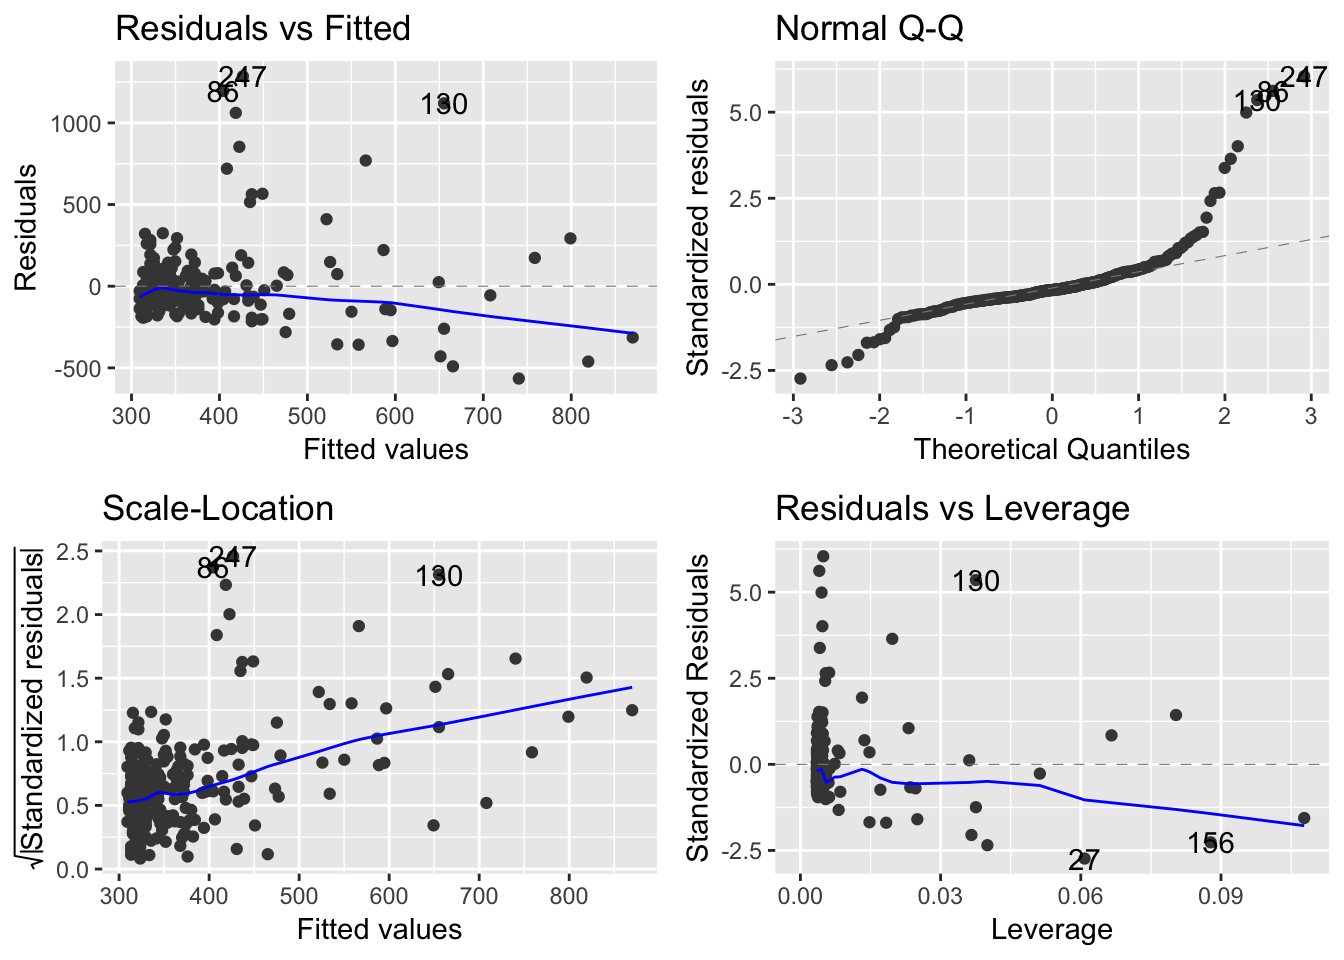
\includegraphics{lecture_modeling_files/figure-latex/unnamed-chunk-8-1.pdf}

\begin{Shaded}
\begin{Highlighting}[]
\CommentTok{## ggplot(pbc, aes(x = bili))+geom_density()}
\end{Highlighting}
\end{Shaded}

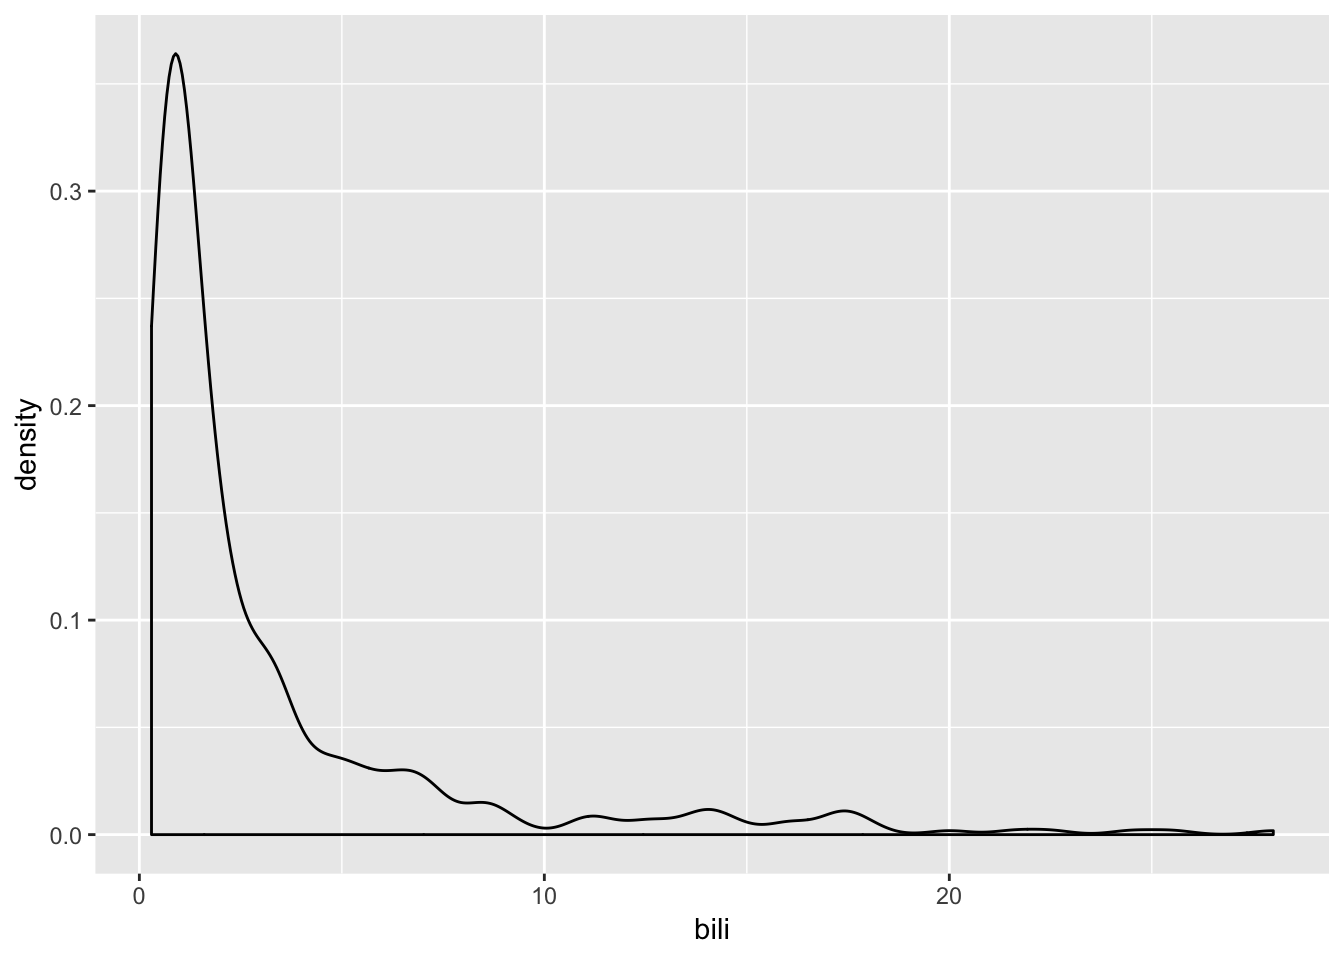
\includegraphics{lecture_modeling_files/figure-latex/unnamed-chunk-10-1.pdf}

\begin{Shaded}
\begin{Highlighting}[]
\CommentTok{## ggplot(pbc, aes(x = log(bili)))+geom_density()}
\end{Highlighting}
\end{Shaded}

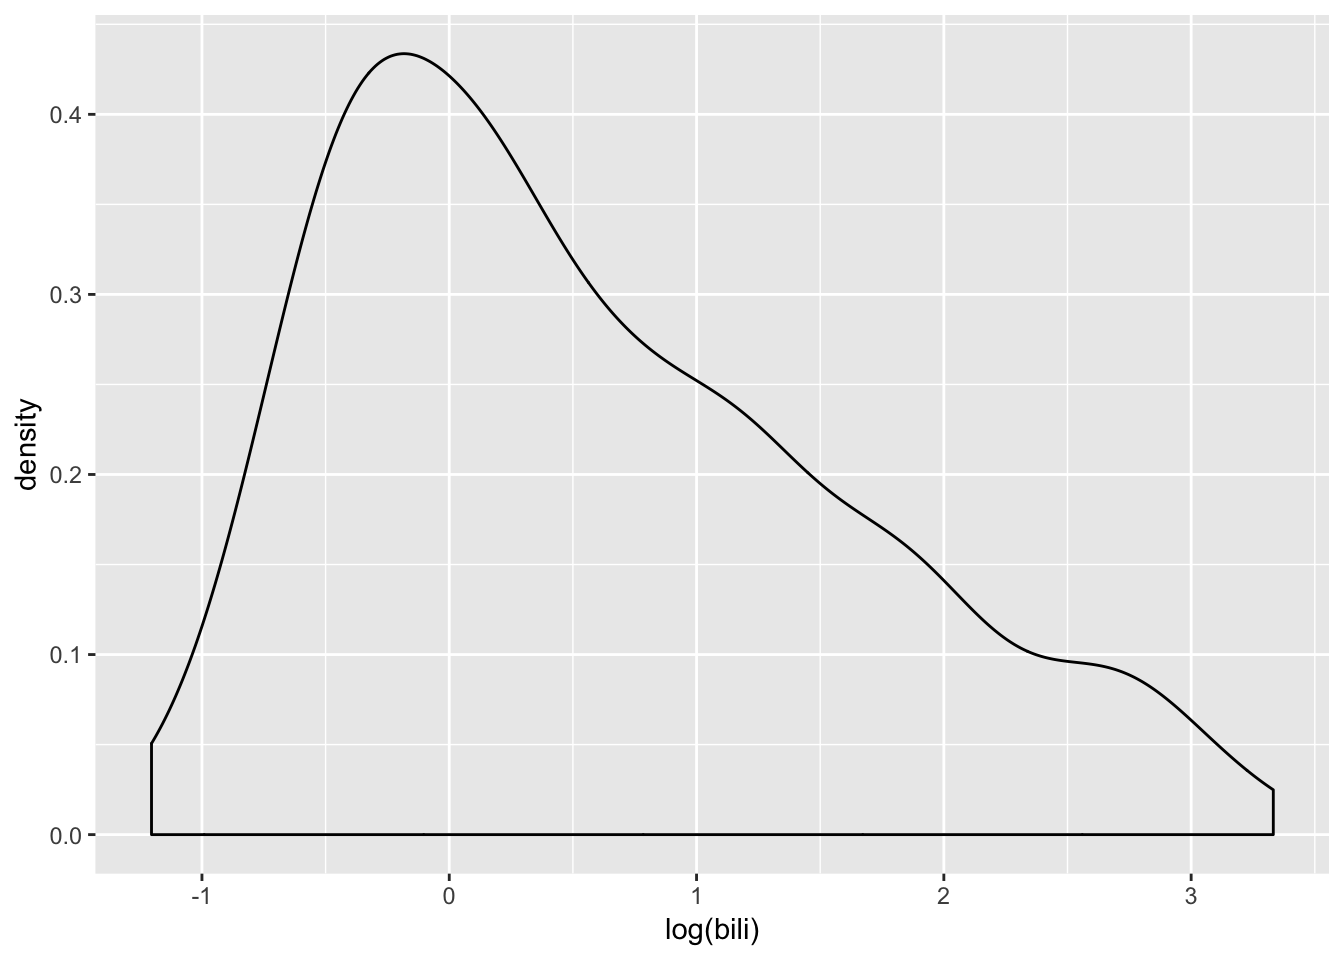
\includegraphics{lecture_modeling_files/figure-latex/unnamed-chunk-12-1.pdf}

\begin{Shaded}
\begin{Highlighting}[]
\NormalTok{myLinearModel2 <-}\StringTok{ }\KeywordTok{lm}\NormalTok{(chol}\OperatorTok{~}\KeywordTok{log}\NormalTok{(bili), }\DataTypeTok{data =}\NormalTok{ pbc)}
\KeywordTok{summary}\NormalTok{(myLinearModel2)}
\end{Highlighting}
\end{Shaded}

\begin{verbatim}

Call:
lm(formula = chol ~ log(bili), data = pbc)

Residuals:
    Min      1Q  Median      3Q     Max 
-440.07  -94.35  -21.07   42.67 1221.86 

Coefficients:
            Estimate Std. Error t value Pr(>|t|)    
(Intercept)   311.48      14.28  21.816  < 2e-16 ***
log(bili)      98.80      12.07   8.186 9.42e-15 ***
---
Signif. codes:  0 '***' 0.001 '**' 0.01 '*' 0.05 '.' 0.1 ' ' 1

Residual standard error: 208.9 on 282 degrees of freedom
  (134 observations deleted due to missingness)
Multiple R-squared:  0.192, Adjusted R-squared:  0.1891 
F-statistic: 67.01 on 1 and 282 DF,  p-value: 9.416e-15
\end{verbatim}

\begin{Shaded}
\begin{Highlighting}[]
\KeywordTok{autoplot}\NormalTok{(myLinearModel2)}
\end{Highlighting}
\end{Shaded}

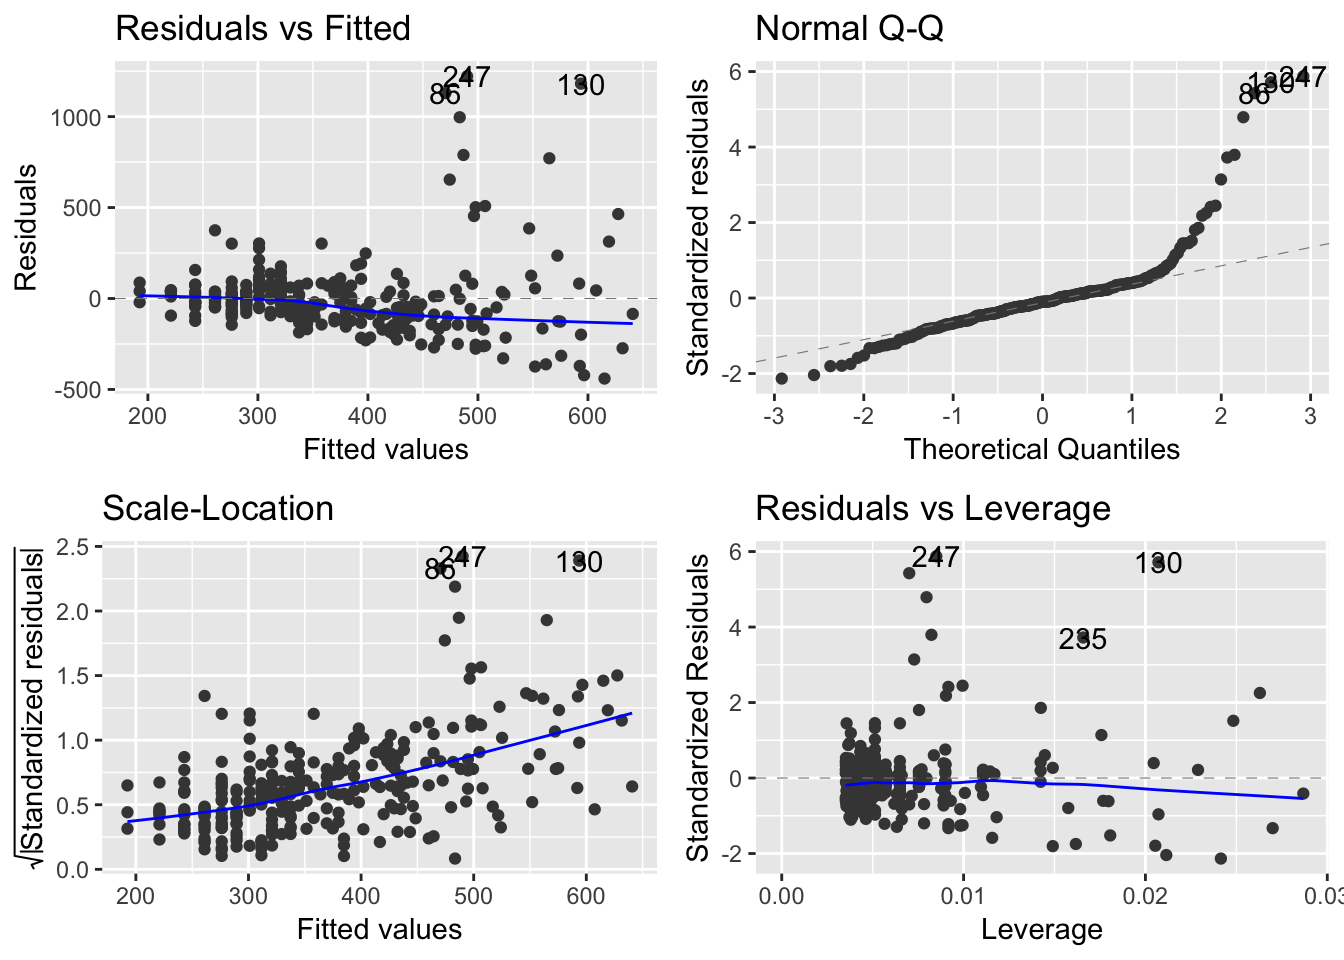
\includegraphics{lecture_modeling_files/figure-latex/unnamed-chunk-14-1.pdf}

\begin{Shaded}
\begin{Highlighting}[]
\KeywordTok{autoplot}\NormalTok{(myLinearModel2, }\DataTypeTok{which=}\DecValTok{1}\NormalTok{)}
\end{Highlighting}
\end{Shaded}

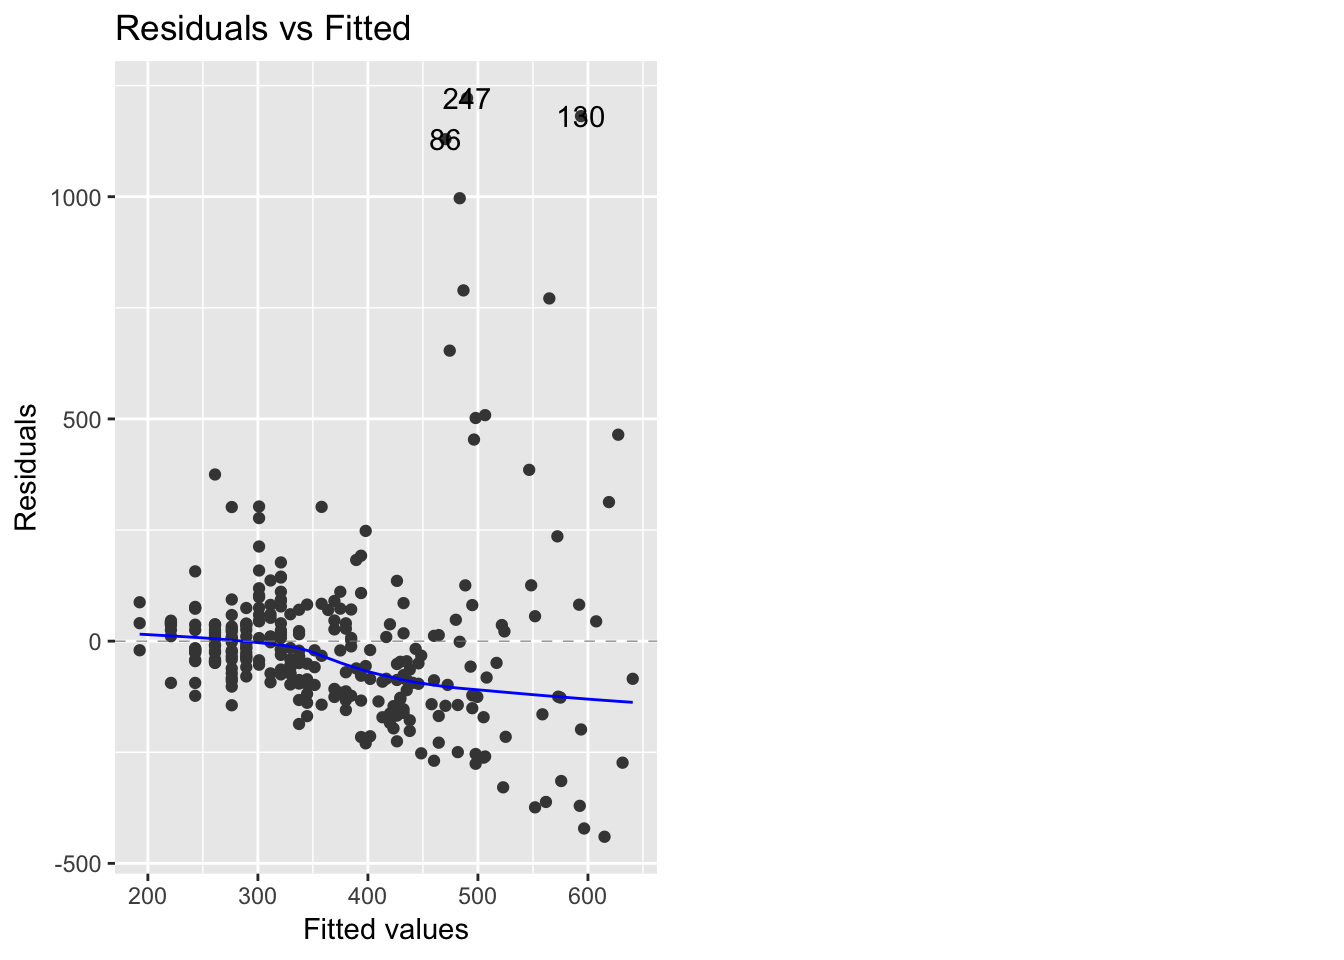
\includegraphics{lecture_modeling_files/figure-latex/unnamed-chunk-15-1.pdf}

\begin{Shaded}
\begin{Highlighting}[]
\NormalTok{d <-}\StringTok{ }\NormalTok{broom}\OperatorTok{::}\KeywordTok{augment}\NormalTok{(myLinearModel2)}
\NormalTok{d}
\end{Highlighting}
\end{Shaded}

\begin{verbatim}
# A tibble: 284 x 10
   .rownames  chol log.bili. .fitted .se.fit .resid    .hat .sigma .cooksd
   <chr>     <int>     <dbl>   <dbl>   <dbl>  <dbl>   <dbl>  <dbl>   <dbl>
 1 1           261    2.67      576.    28.1 -315.  0.0181    208. 2.13e-2
 2 2           302    0.0953    321.    13.7  -18.9 0.00433   209. 1.79e-5
 3 3           176    0.336     345.    12.8 -169.  0.00373   209. 1.23e-3
 4 4           244    0.588     370.    12.4 -126.  0.00352   209. 6.41e-4
 5 5           279    1.22      432.    14.6 -153.  0.00487   209. 1.33e-3
 6 6           248   -0.223     289.    15.8  -41.4 0.00571   209. 1.14e-4
 7 7           322    0         311.    14.3   10.5 0.00467   209. 5.98e-6
 8 8           280   -1.20      193.    24.9   87.5 0.0142    209. 1.28e-3
 9 9           562    1.16      426.    14.2  136.  0.00463   209. 9.84e-4
10 10          200    2.53      562.    26.6 -362.  0.0162    208. 2.51e-2
# ... with 274 more rows, and 1 more variable: .std.resid <dbl>
\end{verbatim}

\begin{Shaded}
\begin{Highlighting}[]
\KeywordTok{ggplot}\NormalTok{(d, }\KeywordTok{aes}\NormalTok{(}\DataTypeTok{x =}\NormalTok{ .fitted, }\DataTypeTok{y =}\NormalTok{ .resid))}\OperatorTok{+}\KeywordTok{geom_point}\NormalTok{()}\OperatorTok{+}\StringTok{ }\KeywordTok{geom_smooth}\NormalTok{(}\DataTypeTok{se=}\NormalTok{F)}\OperatorTok{+}
\StringTok{  }\KeywordTok{labs}\NormalTok{(}\DataTypeTok{x =} \StringTok{'Fitted values'}\NormalTok{, }\DataTypeTok{y =} \StringTok{'Residual values'}\NormalTok{)}
\end{Highlighting}
\end{Shaded}

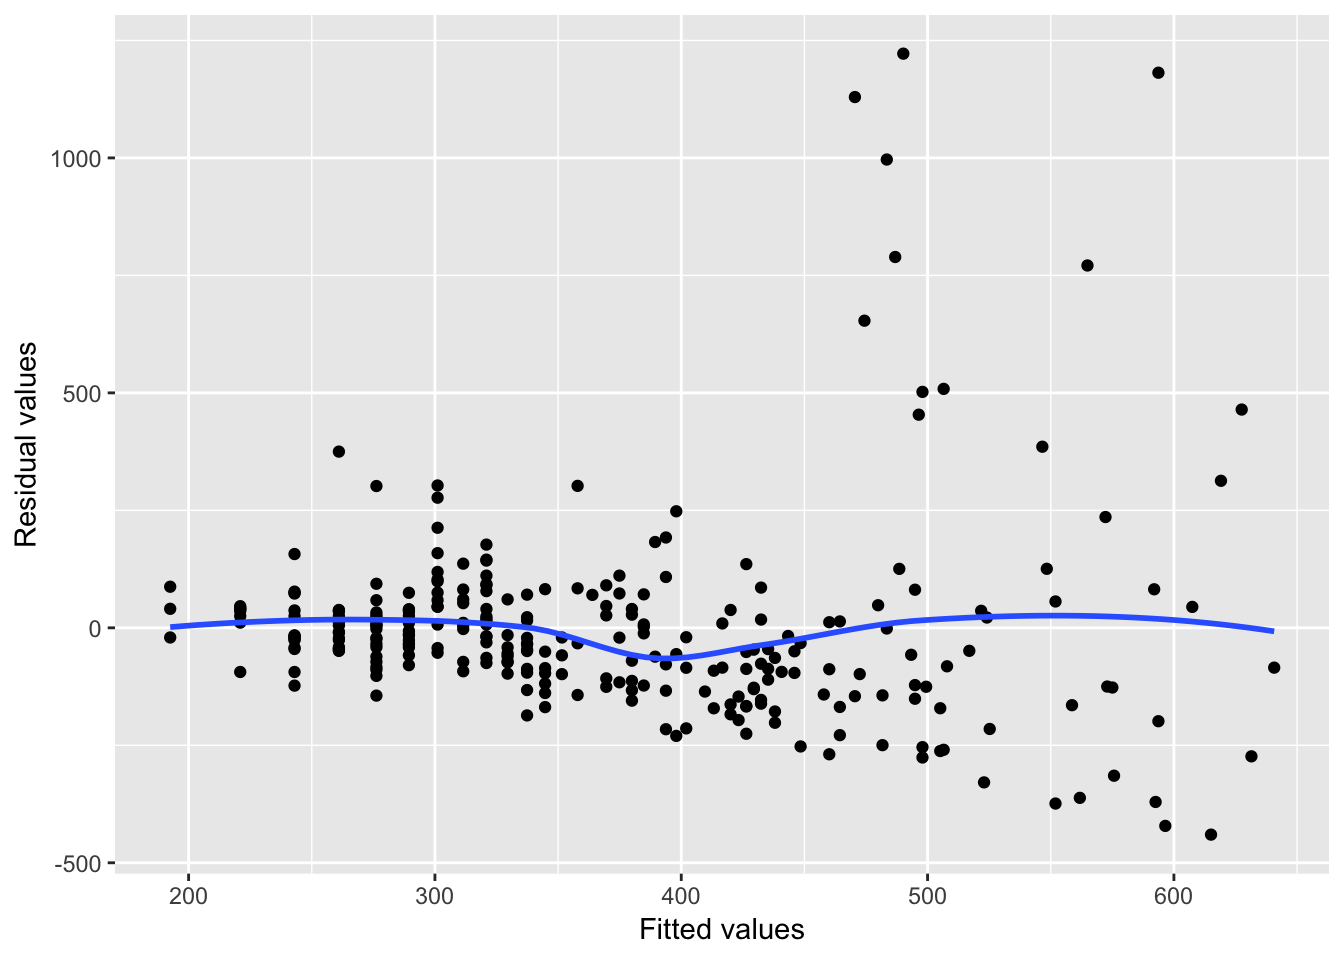
\includegraphics{lecture_modeling_files/figure-latex/unnamed-chunk-17-1.pdf}

\begin{Shaded}
\begin{Highlighting}[]
\KeywordTok{head}\NormalTok{(}\KeywordTok{predict}\NormalTok{(myLinearModel2, }\DataTypeTok{newdata =}\NormalTok{ pbc))}
\end{Highlighting}
\end{Shaded}

\begin{verbatim}
       1        2        3        4        5        6 
575.6925 320.9006 344.7277 369.5578 432.3941 289.4371 
\end{verbatim}

\begin{Shaded}
\begin{Highlighting}[]
\NormalTok{myLM3 <-}\StringTok{ }\KeywordTok{lm}\NormalTok{(chol }\OperatorTok{~}\StringTok{ }\KeywordTok{log}\NormalTok{(bili) }\OperatorTok{+}\StringTok{ }\NormalTok{sex, }\DataTypeTok{data =}\NormalTok{ pbc)}
\NormalTok{broom}\OperatorTok{::}\KeywordTok{tidy}\NormalTok{(myLM3)}
\end{Highlighting}
\end{Shaded}

\begin{verbatim}
# A tibble: 3 x 5
  term        estimate std.error statistic  p.value
  <chr>          <dbl>     <dbl>     <dbl>    <dbl>
1 (Intercept)    283.       36.6     7.71  2.14e-13
2 log(bili)       99.6      12.1     8.22  7.37e-15
3 sexf            32.5      37.8     0.858 3.92e- 1
\end{verbatim}

\begin{Shaded}
\begin{Highlighting}[]
\NormalTok{myLR <-}\StringTok{ }\KeywordTok{glm}\NormalTok{(spiders }\OperatorTok{~}\StringTok{ }\NormalTok{albumin }\OperatorTok{+}\StringTok{ }\NormalTok{bili }\OperatorTok{+}\StringTok{ }\NormalTok{chol, }\DataTypeTok{data =}\NormalTok{ pbc, }\DataTypeTok{family =}\NormalTok{ binomial)}
\NormalTok{myLR}
\end{Highlighting}
\end{Shaded}

\begin{verbatim}

Call:  glm(formula = spiders ~ albumin + bili + chol, family = binomial, 
    data = pbc)

Coefficients:
(Intercept)      albumin         bili         chol  
  2.3326484   -0.9954927    0.0995915   -0.0003176  

Degrees of Freedom: 283 Total (i.e. Null);  280 Residual
  (134 observations deleted due to missingness)
Null Deviance:      341.4 
Residual Deviance: 315.2    AIC: 323.2
\end{verbatim}

\begin{Shaded}
\begin{Highlighting}[]
\NormalTok{broom}\OperatorTok{::}\KeywordTok{tidy}\NormalTok{(myLR)}
\end{Highlighting}
\end{Shaded}

\begin{verbatim}
# A tibble: 4 x 5
  term         estimate std.error statistic p.value
  <chr>           <dbl>     <dbl>     <dbl>   <dbl>
1 (Intercept)  2.33      1.30         1.80  0.0717 
2 albumin     -0.995     0.362       -2.75  0.00595
3 bili         0.0996    0.0344       2.89  0.00381
4 chol        -0.000318  0.000615    -0.517 0.605  
\end{verbatim}

\begin{Shaded}
\begin{Highlighting}[]
\NormalTok{broom}\OperatorTok{::}\KeywordTok{glance}\NormalTok{(myLR)}
\end{Highlighting}
\end{Shaded}

\begin{verbatim}
# A tibble: 1 x 7
  null.deviance df.null logLik   AIC   BIC deviance df.residual
          <dbl>   <int>  <dbl> <dbl> <dbl>    <dbl>       <int>
1          341.     283  -158.  323.  338.     315.         280
\end{verbatim}

\begin{Shaded}
\begin{Highlighting}[]
\KeywordTok{head}\NormalTok{(}\KeywordTok{predict}\NormalTok{(myLR))}
\end{Highlighting}
\end{Shaded}

\begin{verbatim}
          1           2           3           4           5           6 
 1.10554163 -1.77506554 -1.04814132 -0.09414055 -0.93144911 -1.62851203 
\end{verbatim}

\begin{Shaded}
\begin{Highlighting}[]
\KeywordTok{head}\NormalTok{(}\KeywordTok{predict}\NormalTok{(myLR, }\DataTypeTok{type=}\StringTok{'response'}\NormalTok{))}
\end{Highlighting}
\end{Shaded}

\begin{verbatim}
        1         2         3         4         5         6 
0.7512970 0.1449135 0.2595822 0.4764822 0.2826308 0.1640343 
\end{verbatim}

\hypertarget{model-selection}{%
\section{Model selection}\label{model-selection}}

\begin{Shaded}
\begin{Highlighting}[]
\CommentTok{# install.packages('leaps')}
\KeywordTok{library}\NormalTok{(leaps)}
\NormalTok{mtcars1 <-}\StringTok{ }\NormalTok{mtcars }\OperatorTok\StringTok{ }\KeywordTok{mutate_at}\NormalTok{(}\KeywordTok{vars}\NormalTok{(cyl, vs}\OperatorTok{:}\NormalTok{carb), as.factor)}
\NormalTok{all_subsets <-}\StringTok{ }\KeywordTok{regsubsets}\NormalTok{(mpg}\OperatorTok{~}\NormalTok{., }\DataTypeTok{data =}\NormalTok{ mtcars1)}
\NormalTok{all_subsets}
\end{Highlighting}
\end{Shaded}

\begin{verbatim}
Subset selection object
Call: regsubsets.formula(mpg ~ ., data = mtcars1)
16 Variables  (and intercept)
      Forced in Forced out
cyl6      FALSE      FALSE
cyl8      FALSE      FALSE
disp      FALSE      FALSE
hp        FALSE      FALSE
drat      FALSE      FALSE
wt        FALSE      FALSE
qsec      FALSE      FALSE
vs1       FALSE      FALSE
am1       FALSE      FALSE
gear4     FALSE      FALSE
gear5     FALSE      FALSE
carb2     FALSE      FALSE
carb3     FALSE      FALSE
carb4     FALSE      FALSE
carb6     FALSE      FALSE
carb8     FALSE      FALSE
1 subsets of each size up to 8
Selection Algorithm: exhaustive
\end{verbatim}

\begin{Shaded}
\begin{Highlighting}[]
\NormalTok{ind <-}\StringTok{ }\KeywordTok{which.max}\NormalTok{(}\KeywordTok{summary}\NormalTok{(all_subsets)}\OperatorTok{$}\NormalTok{adjr2)}
\KeywordTok{summary}\NormalTok{(all_subsets)}\OperatorTok{$}\NormalTok{which[ind,]}
\end{Highlighting}
\end{Shaded}

\begin{verbatim}
(Intercept)        cyl6        cyl8        disp          hp        drat 
       TRUE        TRUE       FALSE       FALSE        TRUE       FALSE 
         wt        qsec         vs1         am1       gear4       gear5 
       TRUE       FALSE        TRUE        TRUE       FALSE       FALSE 
      carb2       carb3       carb4       carb6       carb8 
      FALSE       FALSE       FALSE       FALSE       FALSE 
\end{verbatim}

\hypertarget{many-models}{%
\section{Many models}\label{many-models}}

\begin{Shaded}
\begin{Highlighting}[]
\NormalTok{mtcars <-}\StringTok{ }\KeywordTok{as_tibble}\NormalTok{(mtcars)}
\NormalTok{mtcars }\OperatorTok\StringTok{ }\KeywordTok{select}\NormalTok{(mpg, disp}\OperatorTok{:}\NormalTok{qsec)}
\end{Highlighting}
\end{Shaded}

\begin{verbatim}
# A tibble: 32 x 6
     mpg  disp    hp  drat    wt  qsec
   <dbl> <dbl> <dbl> <dbl> <dbl> <dbl>
 1  21    160    110  3.9   2.62  16.5
 2  21    160    110  3.9   2.88  17.0
 3  22.8  108     93  3.85  2.32  18.6
 4  21.4  258    110  3.08  3.22  19.4
 5  18.7  360    175  3.15  3.44  17.0
 6  18.1  225    105  2.76  3.46  20.2
 7  14.3  360    245  3.21  3.57  15.8
 8  24.4  147.    62  3.69  3.19  20  
 9  22.8  141.    95  3.92  3.15  22.9
10  19.2  168.   123  3.92  3.44  18.3
# ... with 22 more rows
\end{verbatim}

\begin{Shaded}
\begin{Highlighting}[]
\NormalTok{mtcars }\OperatorTok\StringTok{ }\KeywordTok{select}\NormalTok{(mpg, disp}\OperatorTok{:}\NormalTok{qsec) }\OperatorTok\StringTok{ }
\StringTok{  }\KeywordTok{gather}\NormalTok{(variable, value, }\OperatorTok{-}\NormalTok{mpg)}
\end{Highlighting}
\end{Shaded}

\begin{verbatim}
# A tibble: 160 x 3
     mpg variable value
   <dbl> <chr>    <dbl>
 1  21   disp      160 
 2  21   disp      160 
 3  22.8 disp      108 
 4  21.4 disp      258 
 5  18.7 disp      360 
 6  18.1 disp      225 
 7  14.3 disp      360 
 8  24.4 disp      147.
 9  22.8 disp      141.
10  19.2 disp      168.
# ... with 150 more rows
\end{verbatim}

\begin{Shaded}
\begin{Highlighting}[]
\NormalTok{mtcars }\OperatorTok\StringTok{ }\KeywordTok{select}\NormalTok{(mpg, disp}\OperatorTok{:}\NormalTok{qsec) }\OperatorTok\StringTok{ }
\StringTok{  }\KeywordTok{gather}\NormalTok{(variable, value, }\OperatorTok{-}\NormalTok{mpg) }\OperatorTok\StringTok{ }
\StringTok{  }\KeywordTok{group_by}\NormalTok{(variable) }\OperatorTok\StringTok{ }
\StringTok{  }\KeywordTok{lm}\NormalTok{(mpg}\OperatorTok{~}\NormalTok{value, }\DataTypeTok{data=}\NormalTok{.)}
\end{Highlighting}
\end{Shaded}

\begin{verbatim}

Call:
lm(formula = mpg ~ value, data = .)

Coefficients:
(Intercept)        value  
   21.28328     -0.01483  
\end{verbatim}

\begin{Shaded}
\begin{Highlighting}[]
\NormalTok{mtcars }\OperatorTok\StringTok{ }\KeywordTok{select}\NormalTok{(mpg, disp}\OperatorTok{:}\NormalTok{qsec) }\OperatorTok\StringTok{ }
\StringTok{  }\KeywordTok{gather}\NormalTok{(variable, value, }\OperatorTok{-}\NormalTok{mpg) }\OperatorTok\StringTok{ }
\StringTok{  }\KeywordTok{nest}\NormalTok{(}\OperatorTok{-}\NormalTok{variable)}
\end{Highlighting}
\end{Shaded}

\begin{verbatim}
# A tibble: 5 x 2
  variable data             
  <chr>    <list>           
1 disp     <tibble [32 x 2]>
2 hp       <tibble [32 x 2]>
3 drat     <tibble [32 x 2]>
4 wt       <tibble [32 x 2]>
5 qsec     <tibble [32 x 2]>
\end{verbatim}

\begin{Shaded}
\begin{Highlighting}[]
\NormalTok{bl <-}\StringTok{ }\NormalTok{mtcars }\OperatorTok\StringTok{ }\KeywordTok{select}\NormalTok{(mpg, disp}\OperatorTok{:}\NormalTok{qsec) }\OperatorTok\StringTok{ }
\StringTok{  }\KeywordTok{gather}\NormalTok{(variable, value, }\OperatorTok{-}\NormalTok{mpg) }\OperatorTok\StringTok{ }
\StringTok{  }\KeywordTok{nest}\NormalTok{(}\OperatorTok{-}\NormalTok{variable)}
\NormalTok{bl}\OperatorTok{$}\NormalTok{data[[}\DecValTok{1}\NormalTok{]]}
\end{Highlighting}
\end{Shaded}

\begin{verbatim}
# A tibble: 32 x 2
     mpg value
   <dbl> <dbl>
 1  21    160 
 2  21    160 
 3  22.8  108 
 4  21.4  258 
 5  18.7  360 
 6  18.1  225 
 7  14.3  360 
 8  24.4  147.
 9  22.8  141.
10  19.2  168.
# ... with 22 more rows
\end{verbatim}

\begin{Shaded}
\begin{Highlighting}[]
\NormalTok{mtcars }\OperatorTok\StringTok{ }\KeywordTok{select}\NormalTok{(mpg, disp}\OperatorTok{:}\NormalTok{qsec) }\OperatorTok\StringTok{ }
\StringTok{  }\KeywordTok{gather}\NormalTok{(variable, value, }\OperatorTok{-}\NormalTok{mpg) }\OperatorTok\StringTok{ }
\StringTok{  }\KeywordTok{nest}\NormalTok{(}\OperatorTok{-}\NormalTok{variable) }\OperatorTok\StringTok{ }
\StringTok{  }\KeywordTok{mutate}\NormalTok{(}\DataTypeTok{models =} \KeywordTok{map}\NormalTok{(data, }\OperatorTok{~}\KeywordTok{lm}\NormalTok{(mpg}\OperatorTok{~}\NormalTok{value, }\DataTypeTok{data=}\NormalTok{.)))}
\end{Highlighting}
\end{Shaded}

\begin{verbatim}
# A tibble: 5 x 3
  variable data              models  
  <chr>    <list>            <list>  
1 disp     <tibble [32 x 2]> <S3: lm>
2 hp       <tibble [32 x 2]> <S3: lm>
3 drat     <tibble [32 x 2]> <S3: lm>
4 wt       <tibble [32 x 2]> <S3: lm>
5 qsec     <tibble [32 x 2]> <S3: lm>
\end{verbatim}

\begin{Shaded}
\begin{Highlighting}[]
\NormalTok{ mtcars }\OperatorTok\StringTok{ }\KeywordTok{select}\NormalTok{(mpg, disp}\OperatorTok{:}\NormalTok{qsec) }\OperatorTok\StringTok{ }
\StringTok{  }\KeywordTok{gather}\NormalTok{(variable, value, }\OperatorTok{-}\NormalTok{mpg) }\OperatorTok\StringTok{ }
\StringTok{  }\KeywordTok{nest}\NormalTok{(}\OperatorTok{-}\NormalTok{variable) }\OperatorTok\StringTok{ }
\StringTok{  }\KeywordTok{mutate}\NormalTok{(}\DataTypeTok{models =} \KeywordTok{map}\NormalTok{(data, }\OperatorTok{~}\KeywordTok{lm}\NormalTok{(mpg}\OperatorTok{~}\NormalTok{value, }\DataTypeTok{data=}\NormalTok{.)),}
         \DataTypeTok{outputs =} \KeywordTok{map}\NormalTok{(models, }\OperatorTok{~}\KeywordTok{tidy}\NormalTok{(.)))}
\end{Highlighting}
\end{Shaded}

\begin{verbatim}
# A tibble: 5 x 4
  variable data              models   outputs         
  <chr>    <list>            <list>   <list>          
1 disp     <tibble [32 x 2]> <S3: lm> <tibble [2 x 5]>
2 hp       <tibble [32 x 2]> <S3: lm> <tibble [2 x 5]>
3 drat     <tibble [32 x 2]> <S3: lm> <tibble [2 x 5]>
4 wt       <tibble [32 x 2]> <S3: lm> <tibble [2 x 5]>
5 qsec     <tibble [32 x 2]> <S3: lm> <tibble [2 x 5]>
\end{verbatim}

\begin{Shaded}
\begin{Highlighting}[]
\NormalTok{ mtcars }\OperatorTok\StringTok{ }\KeywordTok{select}\NormalTok{(mpg, disp}\OperatorTok{:}\NormalTok{qsec) }\OperatorTok\StringTok{ }
\StringTok{  }\KeywordTok{gather}\NormalTok{(variable, value, }\OperatorTok{-}\NormalTok{mpg) }\OperatorTok\StringTok{ }
\StringTok{  }\KeywordTok{nest}\NormalTok{(}\OperatorTok{-}\NormalTok{variable) }\OperatorTok\StringTok{ }
\StringTok{  }\KeywordTok{mutate}\NormalTok{(}\DataTypeTok{models =} \KeywordTok{map}\NormalTok{(data, }\OperatorTok{~}\KeywordTok{lm}\NormalTok{(mpg}\OperatorTok{~}\NormalTok{value, }\DataTypeTok{data=}\NormalTok{.)),}
         \DataTypeTok{outputs =} \KeywordTok{map}\NormalTok{(models, }\OperatorTok{~}\KeywordTok{tidy}\NormalTok{(.))) }\OperatorTok\StringTok{ }
\StringTok{  }\KeywordTok{select}\NormalTok{(variable, outputs)}
\end{Highlighting}
\end{Shaded}

\begin{verbatim}
# A tibble: 5 x 2
  variable outputs         
  <chr>    <list>          
1 disp     <tibble [2 x 5]>
2 hp       <tibble [2 x 5]>
3 drat     <tibble [2 x 5]>
4 wt       <tibble [2 x 5]>
5 qsec     <tibble [2 x 5]>
\end{verbatim}

\begin{Shaded}
\begin{Highlighting}[]
\NormalTok{ mtcars }\OperatorTok\StringTok{ }\KeywordTok{select}\NormalTok{(mpg, disp}\OperatorTok{:}\NormalTok{qsec) }\OperatorTok\StringTok{ }
\StringTok{  }\KeywordTok{gather}\NormalTok{(variable, value, }\OperatorTok{-}\NormalTok{mpg) }\OperatorTok\StringTok{ }
\StringTok{  }\KeywordTok{nest}\NormalTok{(}\OperatorTok{-}\NormalTok{variable) }\OperatorTok\StringTok{ }
\StringTok{  }\KeywordTok{mutate}\NormalTok{(}\DataTypeTok{models =} \KeywordTok{map}\NormalTok{(data, }\OperatorTok{~}\KeywordTok{lm}\NormalTok{(mpg}\OperatorTok{~}\NormalTok{value, }\DataTypeTok{data=}\NormalTok{.)),}
         \DataTypeTok{outputs =} \KeywordTok{map}\NormalTok{(models, }\OperatorTok{~}\KeywordTok{tidy}\NormalTok{(.))) }\OperatorTok\StringTok{ }
\StringTok{  }\KeywordTok{select}\NormalTok{(variable, outputs) }\OperatorTok\StringTok{ }
\StringTok{  }\KeywordTok{unnest}\NormalTok{()}
\end{Highlighting}
\end{Shaded}

\begin{verbatim}
# A tibble: 10 x 6
   variable term        estimate std.error statistic  p.value
   <chr>    <chr>          <dbl>     <dbl>     <dbl>    <dbl>
 1 disp     (Intercept)  29.6      1.23       24.1   3.58e-21
 2 disp     value        -0.0412   0.00471    -8.75  9.38e-10
 3 hp       (Intercept)  30.1      1.63       18.4   6.64e-18
 4 hp       value        -0.0682   0.0101     -6.74  1.79e- 7
 5 drat     (Intercept)  -7.52     5.48       -1.37  1.80e- 1
 6 drat     value         7.68     1.51        5.10  1.78e- 5
 7 wt       (Intercept)  37.3      1.88       19.9   8.24e-19
 8 wt       value        -5.34     0.559      -9.56  1.29e-10
 9 qsec     (Intercept)  -5.11    10.0        -0.510 6.14e- 1
10 qsec     value         1.41     0.559       2.53  1.71e- 2
\end{verbatim}

\begin{Shaded}
\begin{Highlighting}[]
\NormalTok{ mtcars }\OperatorTok\StringTok{ }\KeywordTok{select}\NormalTok{(mpg, disp}\OperatorTok{:}\NormalTok{qsec) }\OperatorTok\StringTok{ }
\StringTok{  }\KeywordTok{gather}\NormalTok{(variable, value, }\OperatorTok{-}\NormalTok{mpg) }\OperatorTok\StringTok{ }
\StringTok{  }\KeywordTok{nest}\NormalTok{(}\OperatorTok{-}\NormalTok{variable) }\OperatorTok\StringTok{ }
\StringTok{  }\KeywordTok{mutate}\NormalTok{(}\DataTypeTok{models =} \KeywordTok{map}\NormalTok{(data, }\OperatorTok{~}\KeywordTok{lm}\NormalTok{(mpg}\OperatorTok{~}\NormalTok{value, }\DataTypeTok{data=}\NormalTok{.)),}
         \DataTypeTok{outputs =} \KeywordTok{map}\NormalTok{(models, }\OperatorTok{~}\KeywordTok{tidy}\NormalTok{(.))) }\OperatorTok\StringTok{ }
\StringTok{  }\KeywordTok{select}\NormalTok{(variable, outputs) }\OperatorTok\StringTok{ }
\StringTok{  }\KeywordTok{unnest}\NormalTok{() }\OperatorTok\StringTok{ }
\StringTok{  }\KeywordTok{filter}\NormalTok{(term}\OperatorTok{==}\StringTok{'value'}\NormalTok{)}
\end{Highlighting}
\end{Shaded}

\begin{verbatim}
# A tibble: 5 x 6
  variable term  estimate std.error statistic  p.value
  <chr>    <chr>    <dbl>     <dbl>     <dbl>    <dbl>
1 disp     value  -0.0412   0.00471     -8.75 9.38e-10
2 hp       value  -0.0682   0.0101      -6.74 1.79e- 7
3 drat     value   7.68     1.51         5.10 1.78e- 5
4 wt       value  -5.34     0.559       -9.56 1.29e-10
5 qsec     value   1.41     0.559        2.53 1.71e- 2
\end{verbatim}

\begin{Shaded}
\begin{Highlighting}[]
\NormalTok{ mtcars }\OperatorTok\StringTok{ }\KeywordTok{select}\NormalTok{(mpg, disp}\OperatorTok{:}\NormalTok{qsec) }\OperatorTok\StringTok{ }
\StringTok{  }\KeywordTok{gather}\NormalTok{(variable, value, }\OperatorTok{-}\NormalTok{mpg) }\OperatorTok\StringTok{ }
\StringTok{  }\KeywordTok{nest}\NormalTok{(}\OperatorTok{-}\NormalTok{variable) }\OperatorTok\StringTok{ }
\StringTok{  }\KeywordTok{mutate}\NormalTok{(}\DataTypeTok{models =} \KeywordTok{map}\NormalTok{(data, }\OperatorTok{~}\KeywordTok{lm}\NormalTok{(mpg}\OperatorTok{~}\NormalTok{value, }\DataTypeTok{data=}\NormalTok{.)),}
         \DataTypeTok{outputs =} \KeywordTok{map}\NormalTok{(models, }\OperatorTok{~}\KeywordTok{tidy}\NormalTok{(.))) }\OperatorTok\StringTok{ }
\StringTok{  }\KeywordTok{select}\NormalTok{(variable, outputs) }\OperatorTok\StringTok{ }
\StringTok{  }\KeywordTok{unnest}\NormalTok{() }\OperatorTok\StringTok{ }
\StringTok{  }\KeywordTok{filter}\NormalTok{(term}\OperatorTok{==}\StringTok{'value'}\NormalTok{) }\OperatorTok\StringTok{ }
\StringTok{  }\KeywordTok{mutate_if}\NormalTok{(is.numeric, }\KeywordTok{funs}\NormalTok{(}\KeywordTok{round}\NormalTok{(., }\DecValTok{3}\NormalTok{)))}
\end{Highlighting}
\end{Shaded}

\begin{verbatim}
# A tibble: 5 x 6
  variable term  estimate std.error statistic p.value
  <chr>    <chr>    <dbl>     <dbl>     <dbl>   <dbl>
1 disp     value   -0.041     0.005     -8.75   0    
2 hp       value   -0.068     0.01      -6.74   0    
3 drat     value    7.68      1.51       5.10   0    
4 wt       value   -5.34      0.559     -9.56   0    
5 qsec     value    1.41      0.559      2.52   0.017
\end{verbatim}

\hypertarget{predictive-modeling}{%
\chapter{Predictive modeling}\label{predictive-modeling}}

\begin{Shaded}
\begin{Highlighting}[]
\KeywordTok{library}\NormalTok{(tidyverse)}
\KeywordTok{library}\NormalTok{(caret)}
\KeywordTok{data}\NormalTok{(diamonds)}
\KeywordTok{set.seed}\NormalTok{(}\DecValTok{12356}\NormalTok{)}
\NormalTok{diamonds_train <-}\StringTok{ }\NormalTok{diamonds }\OperatorTok\StringTok{ }\KeywordTok{sample_frac}\NormalTok{(}\DataTypeTok{size =} \FloatTok{0.8}\NormalTok{) }\CommentTok{# 80%}
\NormalTok{diamonds_test <-}\StringTok{ }\KeywordTok{anti_join}\NormalTok{(diamonds, diamonds_train)}
\NormalTok{(}\KeywordTok{nrow}\NormalTok{(diamonds) }\OperatorTok{==}\StringTok{ }\KeywordTok{nrow}\NormalTok{(diamonds_train) }\OperatorTok{+}\StringTok{ }\KeywordTok{nrow}\NormalTok{(diamonds_test))}
\end{Highlighting}
\end{Shaded}

\begin{verbatim}
[1] FALSE
\end{verbatim}


\end{document}
